\documentclass{article}
\usepackage[paperwidth=14in,paperheight=7.9in,margin=0.22in]{geometry}
\usepackage{amsmath,amssymb}
\usepackage{tikz}
\usetikzlibrary{arrows.meta,calc,decorations.pathreplacing,positioning}
\pagestyle{empty}
\setlength{\parindent}{0pt}

\AddToHook{shipout/foreground}{%
  \begin{tikzpicture}[remember picture,overlay]
    \node[anchor=south east, font=\small, text=black!55]
      at ([xshift=-5mm,yshift=3mm]current page.south east) {\thepage};
  \end{tikzpicture}%
}

\newcommand{\ket}[1]{\left\lvert #1\right\rangle}
\definecolor{gateblue}{RGB}{242,246,251}
\definecolor{lookorange}{RGB}{255,245,231}
\definecolor{addviolet}{RGB}{244,242,251}
\definecolor{outgreen}{RGB}{239,248,242}

\tikzset{
  wire/.style={black, line width=0.9pt},
  omitted/.style={black, line width=0.9pt, dashed},
  gate/.style={draw=black, line width=0.9pt, fill=gateblue,
               minimum height=10mm, rounded corners=1pt,
               inner sep=4pt, align=center, font=\normalsize},
  lookup/.style={draw=black, line width=0.9pt, fill=lookorange,
                 minimum height=8mm, rounded corners=1pt,
                 inner sep=4pt, align=center, font=\normalsize},
  add/.style={draw=black, line width=0.9pt, fill=addviolet,
              minimum height=9mm, rounded corners=1pt,
              inner sep=4pt, align=center, font=\normalsize},
  phase/.style={draw=black, line width=0.9pt, fill=gateblue,
                minimum height=35mm, text width=45mm,
                rounded corners=1pt, inner sep=5pt,
                align=center, font=\small},
  phaseviolet/.style={phase, fill=addviolet},
  phaseorange/.style={phase, fill=lookorange},
  lab/.style={font=\large},
  smalllab/.style={font=\normalsize},
  note/.style={font=\small, text=black!75},
  flow/.style={-{Latex[length=2mm,width=1.2mm]}, line width=0.8pt},
  detail/.style={draw=black, line width=0.9pt, fill=gateblue,
                 minimum height=15mm, text width=42mm,
                 rounded corners=1pt, inner sep=5pt,
                 align=center, font=\normalsize},
  detailviolet/.style={detail, fill=addviolet},
  detailorange/.style={detail, fill=lookorange},
  detailgreen/.style={detail, fill=outgreen},
  registerbox/.style={draw=black!55, line width=0.7pt, fill=white,
                      rounded corners=1pt, inner sep=5pt,
                      align=center, font=\normalsize},
}

\begin{document}

% ============================================================================
% Page 1: full ECDLP circuit with the U_f window wiring expanded
% ============================================================================
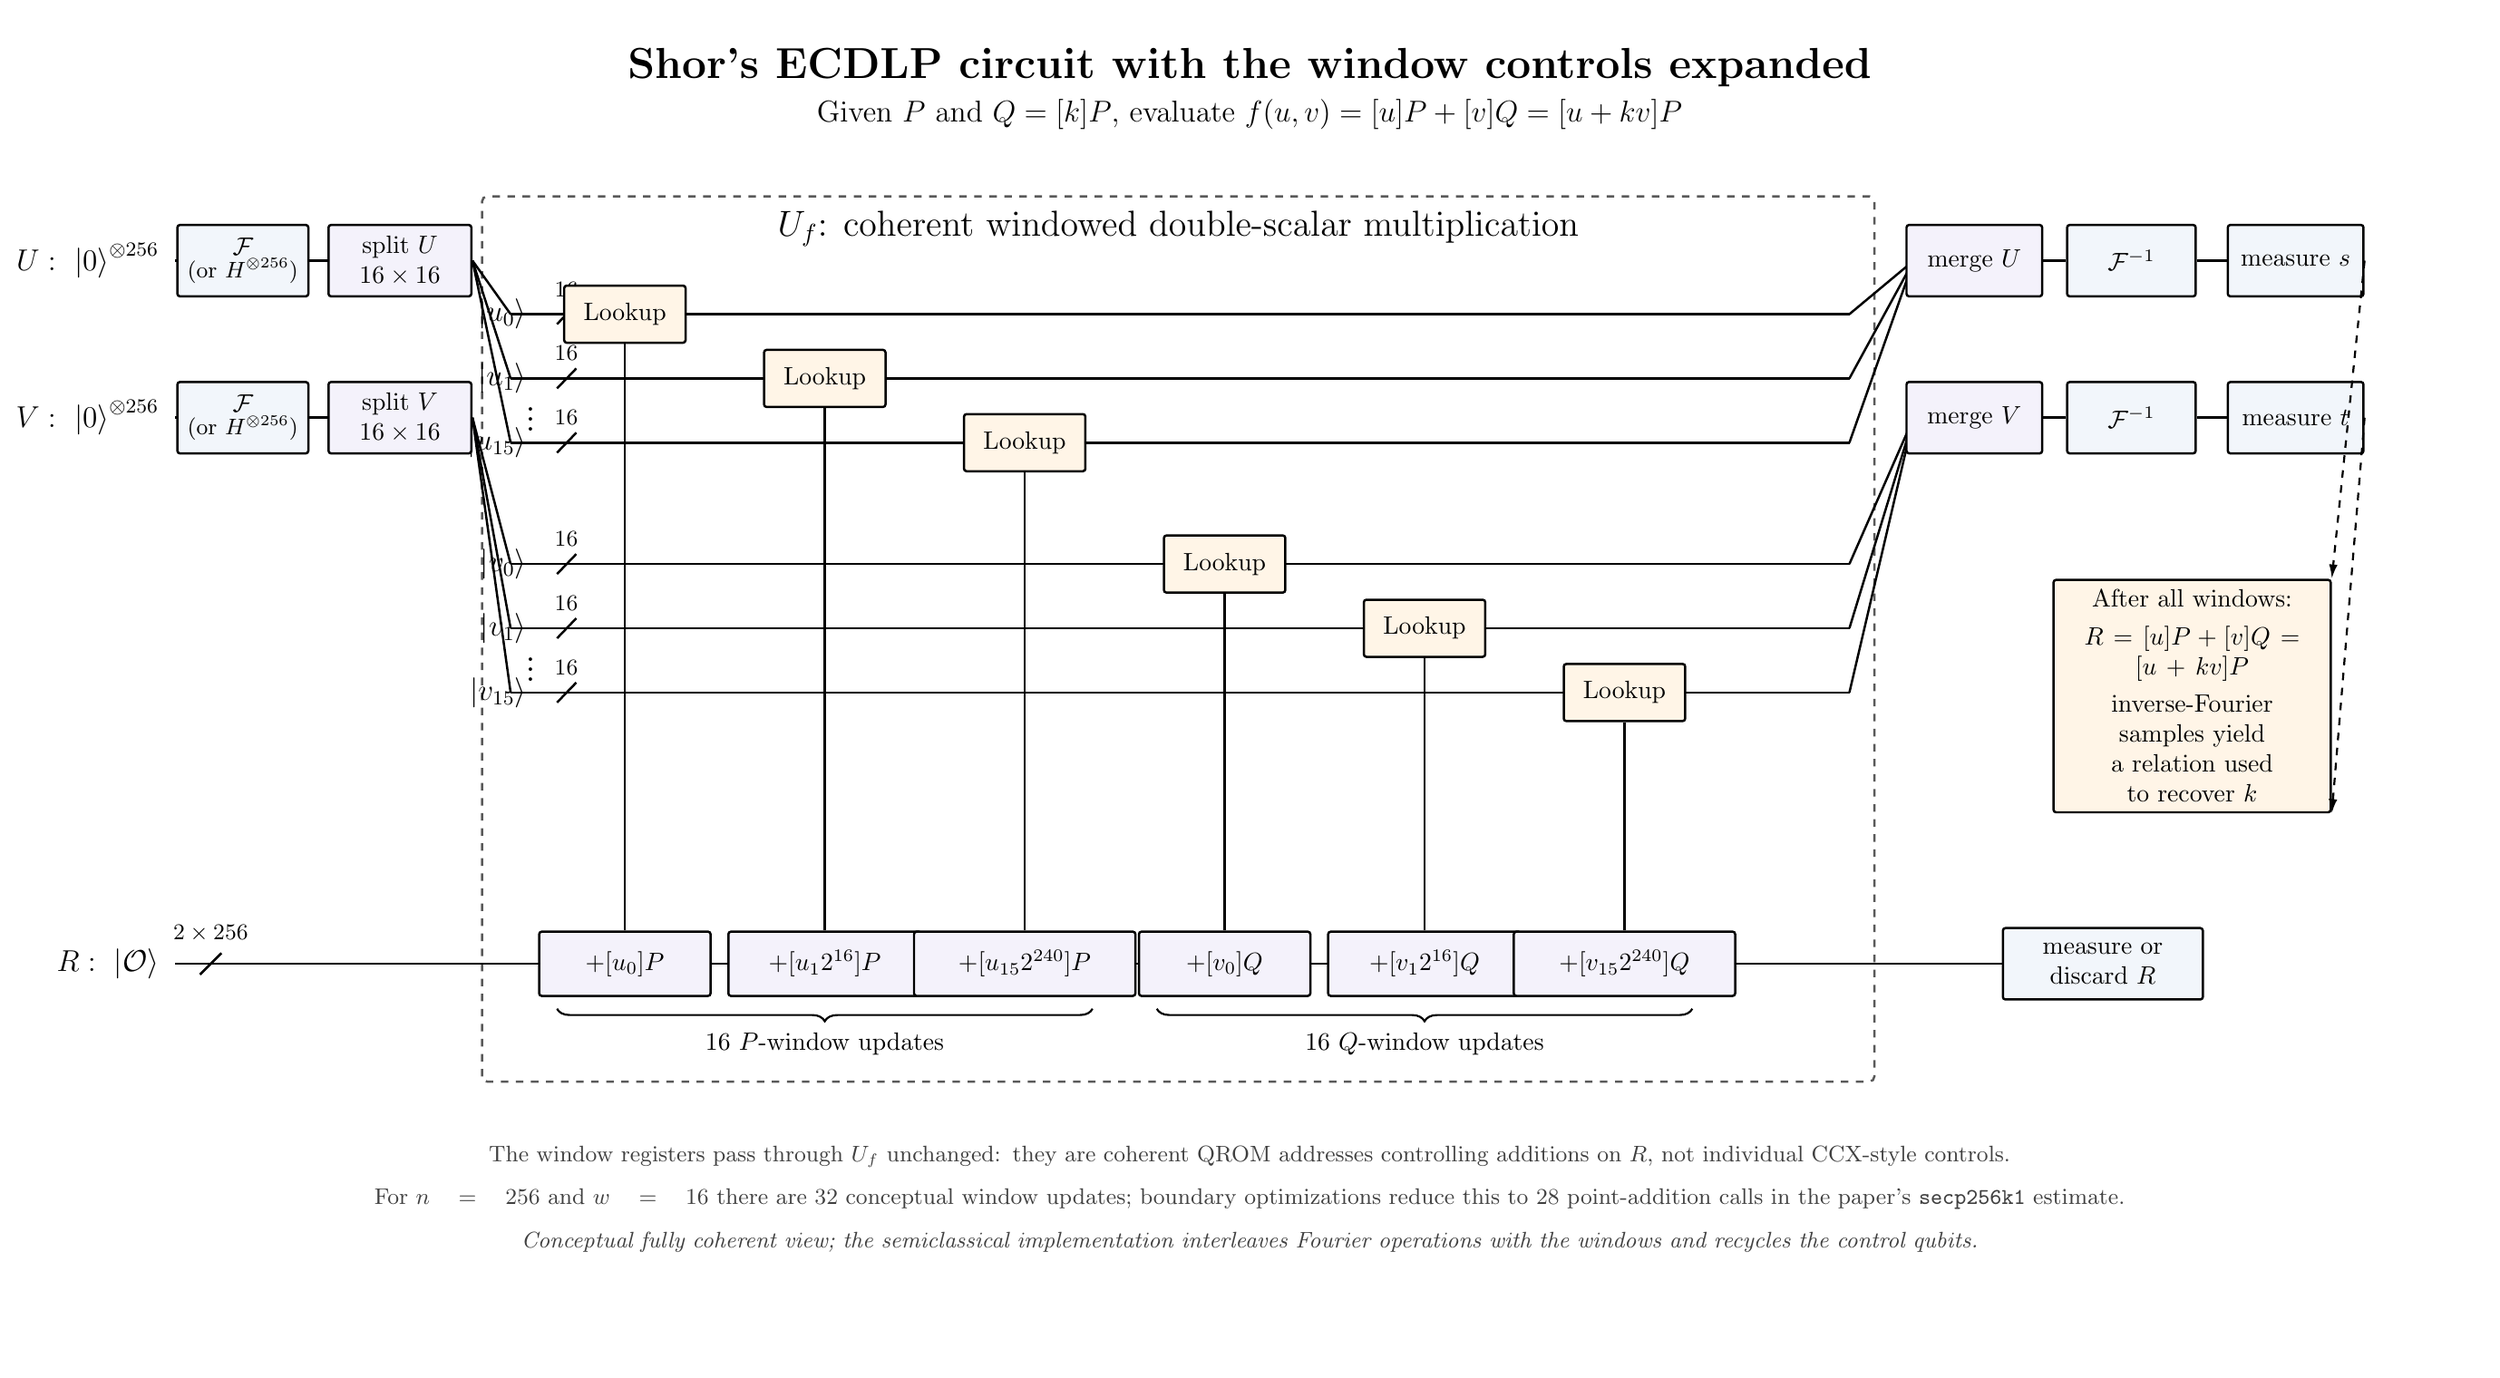
\begin{tikzpicture}[x=1cm,y=1cm]
  \path[use as bounding box] (0,0) rectangle (34.3,18.6);

  \node[font=\LARGE\bfseries] at (17.15,18.0)
    {Shor's ECDLP circuit with the window controls expanded};
  \node[font=\large] at (17.15,17.35)
    {Given $P$ and $Q=[k]P$, evaluate $f(u,v)=[u]P+[v]Q=[u+kv]P$};

  % Preparation and readout buses.
  \node[lab, anchor=east] at (2.0,15.3) {$U:\ \ket{0}^{\otimes 256}$};
  \node[lab, anchor=east] at (2.0,13.1) {$V:\ \ket{0}^{\otimes 256}$};
  \draw[wire] (2.1,15.3) -- (2.15,15.3);
  \draw[wire] (2.1,13.1) -- (2.15,13.1);
  \node[gate, minimum width=18mm] (fu) at (3.05,15.3)
    {$\mathcal F$\\[-1mm]{\small(or $H^{\otimes256}$)}};
  \node[gate, minimum width=18mm] (fv) at (3.05,13.1)
    {$\mathcal F$\\[-1mm]{\small(or $H^{\otimes256}$)}};
  \draw[wire] (fu.east) -- (4.25,15.3);
  \draw[wire] (fv.east) -- (4.25,13.1);
  \node[gate, fill=addviolet, minimum width=20mm] (splitu) at (5.25,15.3)
    {split $U$\\$16\times16$};
  \node[gate, fill=addviolet, minimum width=20mm] (splitv) at (5.25,13.1)
    {split $V$\\$16\times16$};

  % U_f boundary.
  \draw[black!65, line width=0.9pt, dashed, rounded corners=2pt]
    (6.4,3.8) rectangle (25.9,16.2);
  \node[font=\Large] at (16.15,15.75)
    {$U_f$: coherent windowed double-scalar multiplication};

  % Representative U windows.
  \foreach \name/\yy/\xx in {u_0/14.55/8.4,u_1/13.65/11.2,u_{15}/12.75/14.0}{
    \draw[wire] (6.8,\yy) -- (25.55,\yy);
    \node[lab, anchor=east] at (7.15,\yy) {$\ket{\name}$};
    \draw[wire] (7.45,\yy-0.14) -- (7.72,\yy+0.14);
    \node[font=\small] at (7.58,\yy+0.35) {$16$};
    \node[lookup, minimum width=17mm] (L\name) at (\xx,\yy) {Lookup};
  }
  \node[font=\Large] at (7.08,13.18) {$\vdots$};

  % Representative V windows.
  \foreach \name/\yy/\xx in {v_0/11.05/16.8,v_1/10.15/19.6,v_{15}/9.25/22.4}{
    \draw[wire] (6.8,\yy) -- (25.55,\yy);
    \node[lab, anchor=east] at (7.15,\yy) {$\ket{\name}$};
    \draw[wire] (7.45,\yy-0.14) -- (7.72,\yy+0.14);
    \node[font=\small] at (7.58,\yy+0.35) {$16$};
    \node[lookup, minimum width=17mm] (L\name) at (\xx,\yy) {Lookup};
  }
  \node[font=\Large] at (7.08,9.68) {$\vdots$};

  % Split and merge fanout, showing that the windows are preserved.
  \foreach \yy in {14.55,13.65,12.75}{
    \draw[wire] (splitu.east) -- (6.8,\yy);
    \draw[wire] (25.55,\yy) -- (26.45,15.3);
  }
  \foreach \yy in {11.05,10.15,9.25}{
    \draw[wire] (splitv.east) -- (6.8,\yy);
    \draw[wire] (25.55,\yy) -- (26.45,13.1);
  }

  % Accumulator and representative additions.
  \node[lab, anchor=east] at (2.0,5.45) {$R:\ \ket{\mathcal O}$};
  \draw[wire] (2.1,5.45) -- (28.9,5.45);
  \draw[wire] (2.45,5.30) -- (2.75,5.60);
  \node[font=\small] at (2.60,5.88) {$2\times256$};

  \node[add, minimum width=24mm] (A0) at (8.4,5.45) {$+[u_0]P$};
  \node[add, minimum width=27mm] (A1) at (11.2,5.45) {$+[u_1 2^{16}]P$};
  \node[add, minimum width=31mm] (A15) at (14.0,5.45) {$+[u_{15}2^{240}]P$};
  \node[add, minimum width=24mm] (B0) at (16.8,5.45) {$+[v_0]Q$};
  \node[add, minimum width=27mm] (B1) at (19.6,5.45) {$+[v_1 2^{16}]Q$};
  \node[add, minimum width=31mm] (B15) at (22.4,5.45) {$+[v_{15}2^{240}]Q$};

  \draw[wire] (Lu_0.south) -- (A0.north);
  \draw[wire] (Lu_1.south) -- (A1.north);
  \draw[wire] (Lu_{15}.south) -- (A15.north);
  \draw[wire] (Lv_0.south) -- (B0.north);
  \draw[wire] (Lv_1.south) -- (B1.north);
  \draw[wire] (Lv_{15}.south) -- (B15.north);

  \draw[decorate, decoration={brace, amplitude=5pt}, line width=0.8pt]
    (14.95,4.82) -- (7.45,4.82)
    node[midway, below=6pt, font=\normalsize] {$16$ $P$-window updates};
  \draw[decorate, decoration={brace, amplitude=5pt}, line width=0.8pt]
    (23.35,4.82) -- (15.85,4.82)
    node[midway, below=6pt, font=\normalsize] {$16$ $Q$-window updates};

  % Fourier readout.
  \node[gate, fill=addviolet, minimum width=19mm] (mergeu) at (27.3,15.3) {merge $U$};
  \node[gate, fill=addviolet, minimum width=19mm] (mergev) at (27.3,13.1) {merge $V$};
  \node[gate, minimum width=18mm] (ifu) at (29.5,15.3) {$\mathcal F^{-1}$};
  \node[gate, minimum width=18mm] (ifv) at (29.5,13.1) {$\mathcal F^{-1}$};
  \node[gate, minimum width=19mm] (mu) at (31.8,15.3) {measure $s$};
  \node[gate, minimum width=19mm] (mv) at (31.8,13.1) {measure $t$};
  \draw[wire] (mergeu.east) -- (ifu.west);
  \draw[wire] (mergev.east) -- (ifv.west);
  \draw[wire] (ifu.east) -- (mu.west);
  \draw[wire] (ifv.east) -- (mv.west);

  \node[gate, minimum width=28mm] at (29.1,5.45) {measure or\\discard $R$};
  \node[lookup, text width=36mm, minimum height=28mm] (post) at (30.35,9.2)
    {After all windows:\\[1mm]
     $R=[u]P+[v]Q=[u+kv]P$\\[1mm]
     inverse-Fourier samples yield\\a relation used to recover $k$};
  \draw[flow, dashed] (mu.east) -- (post.north east);
  \draw[flow, dashed] (mv.east) -- (post.south east);

  \node[note, text width=29cm, align=center] at (17.15,2.75)
    {The window registers pass through $U_f$ unchanged: they are coherent QROM addresses controlling additions on $R$, not individual CCX-style controls.};
  \node[note, text width=29cm, align=center] at (17.15,2.15)
    {For $n=256$ and $w=16$ there are $32$ conceptual window updates; boundary optimizations reduce this to $28$ point-addition calls in the paper's \texttt{secp256k1} estimate.};
  \node[note, text width=29cm, align=center, font=\small\itshape] at (17.15,1.55)
    {Conceptual fully coherent view; the semiclassical implementation interleaves Fourier operations with the windows and recycles the control qubits.};
\end{tikzpicture}

\newpage

% ============================================================================
% Page 2: generic in-place point addition and its Shor-window interpretation
% ============================================================================
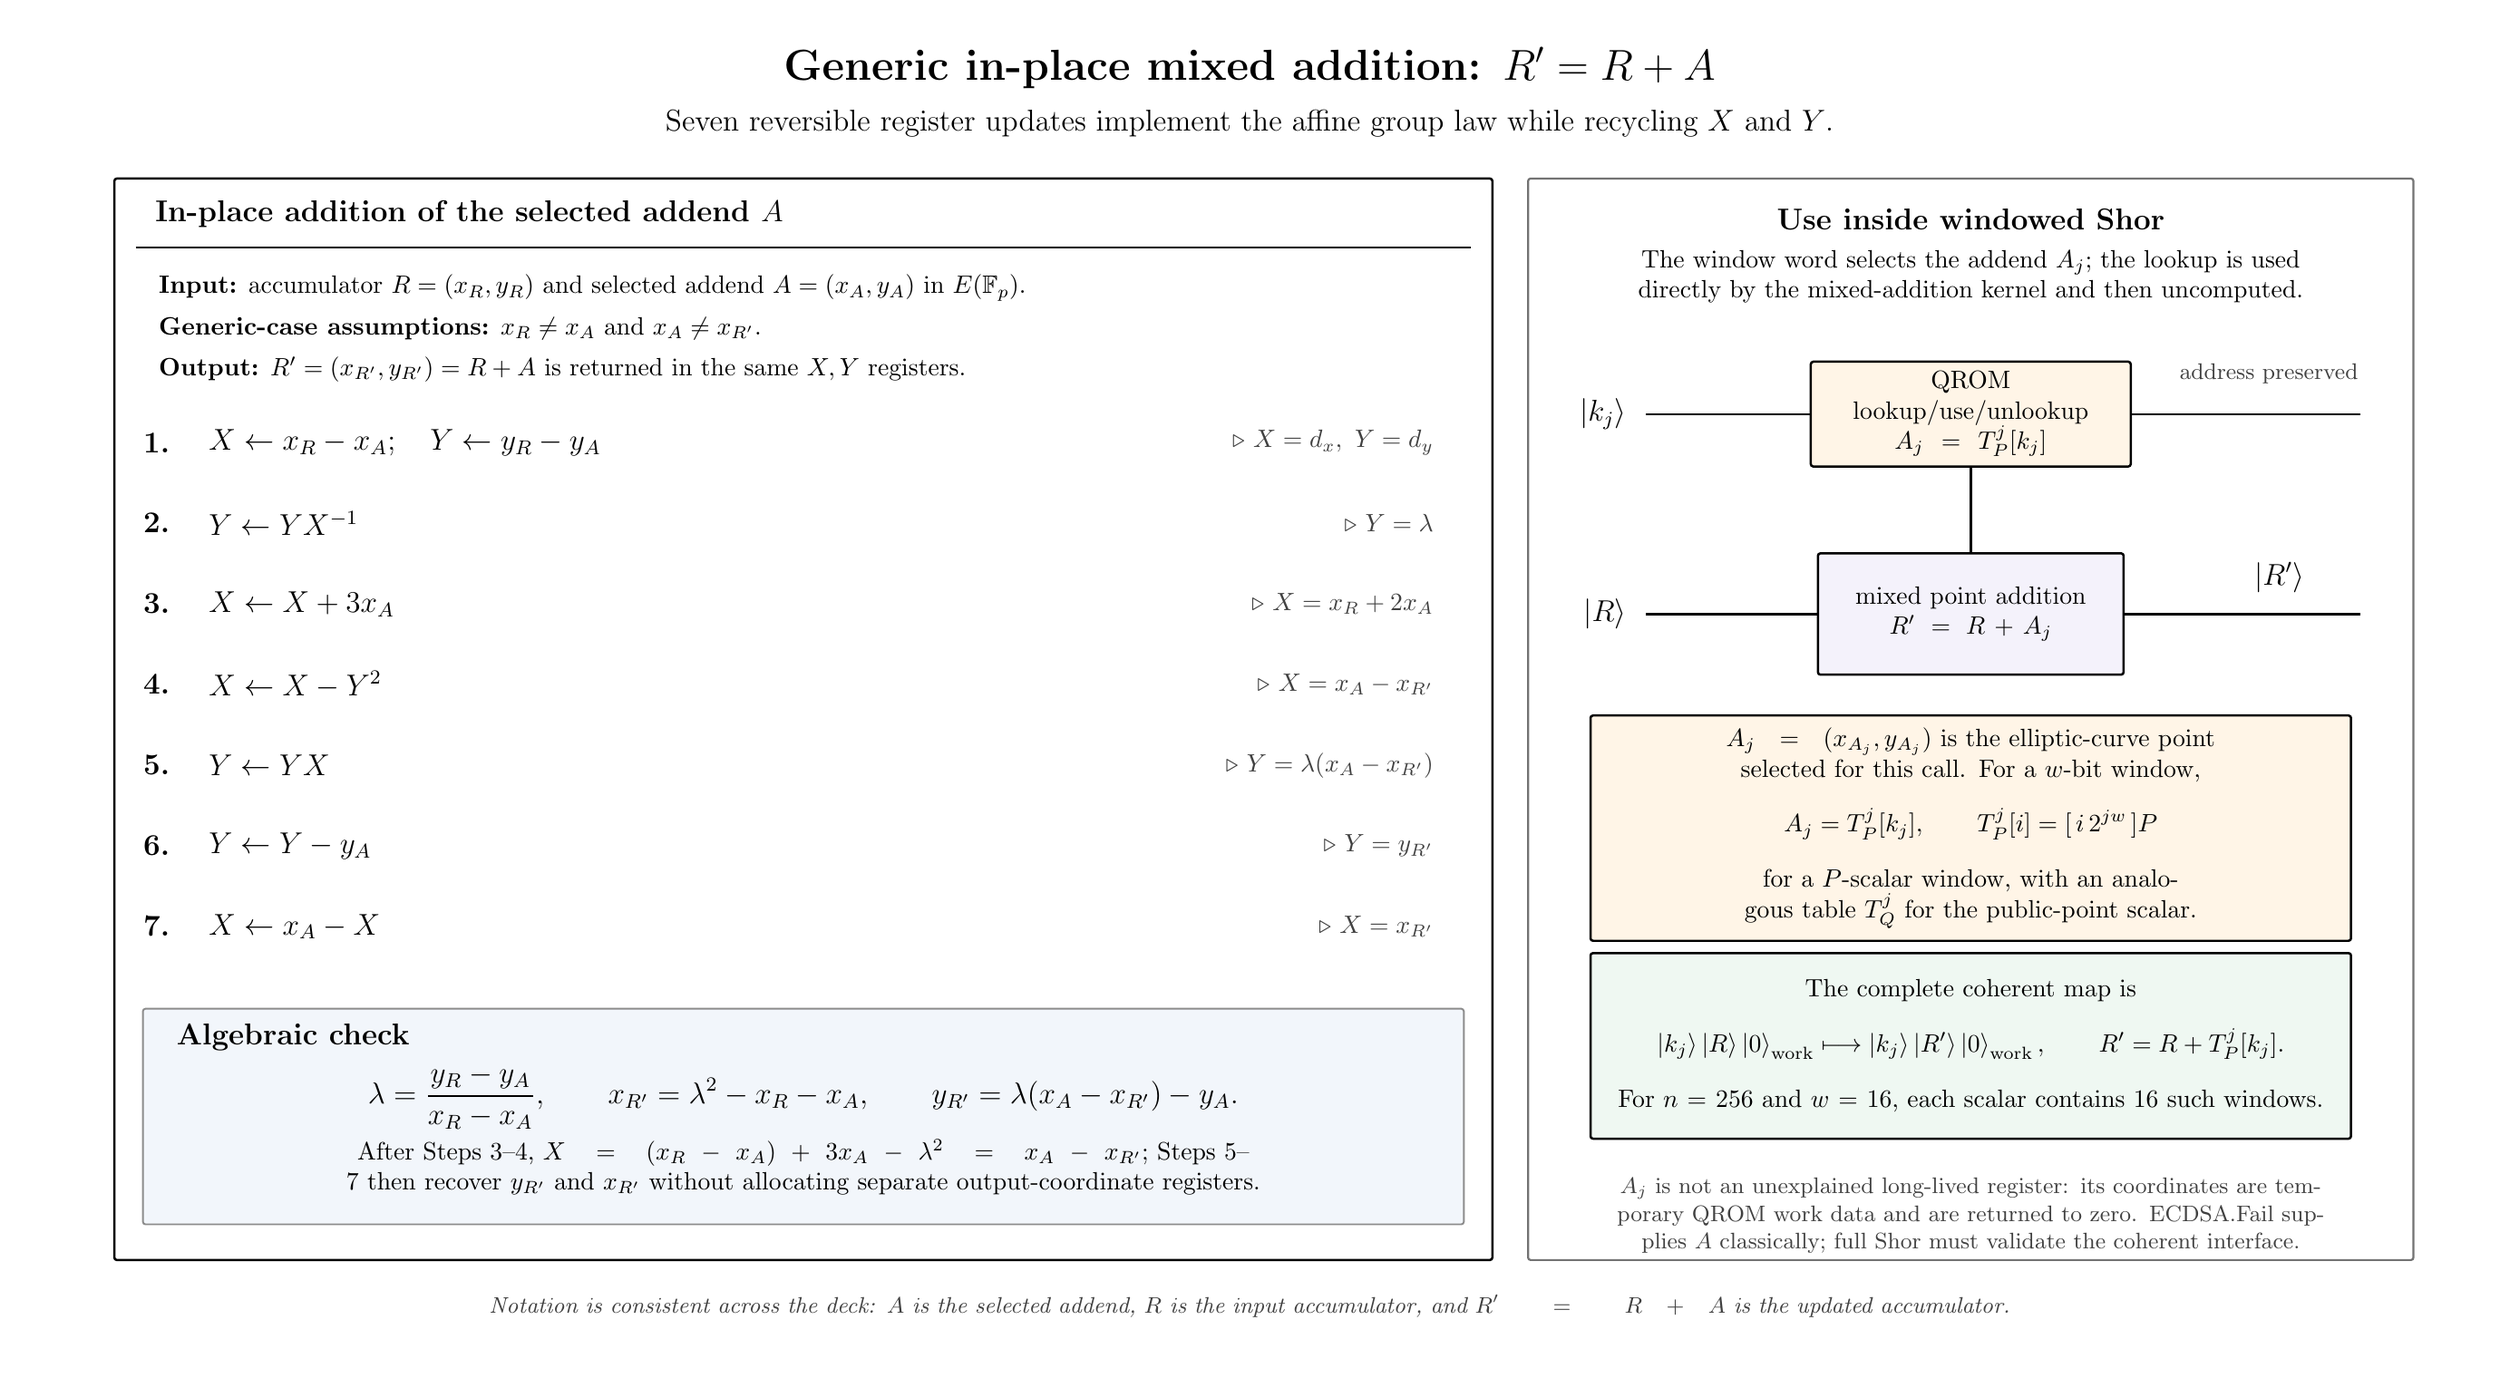
\begin{tikzpicture}[x=1cm,y=1cm]
  \path[use as bounding box] (0,0) rectangle (34.3,18.6);

  \node[font=\LARGE\bfseries] at (17.15,18.0)
    {Generic in-place mixed addition: $R'=R+A$};
  \node[font=\large] at (17.15,17.22)
    {Seven reversible register updates implement the affine group law while recycling $X$ and $Y$.};

  % Algorithm panel.
  \draw[black, line width=0.9pt, rounded corners=1pt]
    (1.25,1.30) rectangle (20.55,16.45);
  \node[font=\large\bfseries, anchor=west] at (1.70,15.95)
    {In-place addition of the selected addend $A$};
  \draw[black, line width=0.7pt] (1.55,15.48) -- (20.25,15.48);

  \node[font=\normalsize, anchor=west] at (1.75,14.92)
    {\textbf{Input:} accumulator $R=(x_R,y_R)$ and selected addend $A=(x_A,y_A)$ in $E(\mathbb F_p)$.};
  \node[font=\normalsize, anchor=west] at (1.75,14.35)
    {\textbf{Generic-case assumptions:} $x_R\neq x_A$ and $x_A\neq x_{R'}$.};
  \node[font=\normalsize, anchor=west] at (1.75,13.78)
    {\textbf{Output:} $R'=(x_{R'},y_{R'})=R+A$ is returned in the same $X,Y$ registers.};

  \foreach \num/\yy/\op/\comment in {
    1/12.75/{X\gets x_R-x_A;\quad Y\gets y_R-y_A}/{X=d_x,\ Y=d_y},
    2/11.62/{Y\gets YX^{-1}}/{Y=\lambda},
    3/10.49/{X\gets X+3x_A}/{X=x_R+2x_A},
    4/9.36/{X\gets X-Y^2}/{X=x_A-x_{R'}},
    5/8.23/{Y\gets YX}/{Y=\lambda(x_A-x_{R'})},
    6/7.10/{Y\gets Y-y_A}/{Y=y_{R'}},
    7/5.97/{X\gets x_A-X}/{X=x_{R'}}
  }{
    \node[font=\large\bfseries, anchor=east] at (2.15,\yy) {\num.};
    \node[font=\large, anchor=west] at (2.45,\yy) {$\op$};
    \node[font=\normalsize, anchor=east, text=black!75] at (19.85,\yy)
      {$\triangleright\ \comment$};
  }

  \draw[black!45, line width=0.7pt, rounded corners=1pt, fill=gateblue]
    (1.65,1.80) rectangle (20.15,4.82);
  \node[font=\large\bfseries, anchor=west] at (2.00,4.42)
    {Algebraic check};
  \node[font=\large] at (10.90,3.58)
    {$\displaystyle
      \lambda=\frac{y_R-y_A}{x_R-x_A},\qquad
      x_{R'}=\lambda^2-x_R-x_A,\qquad
      y_{R'}=\lambda(x_A-x_{R'})-y_A.$};
  \node[font=\normalsize, text width=17.2cm, align=center] at (10.90,2.60)
    {After Steps 3--4,
     $X=(x_R-x_A)+3x_A-\lambda^2=x_A-x_{R'}$; Steps 5--7 then recover
     $y_{R'}$ and $x_{R'}$ without allocating separate output-coordinate registers.};

  % Shor-window context panel.
  \draw[black!55, line width=0.8pt, rounded corners=1pt]
    (21.05,1.30) rectangle (33.45,16.45);
  \node[font=\large\bfseries] at (27.25,15.88)
    {Use inside windowed Shor};
  \node[font=\normalsize, text width=11.2cm, align=center] at (27.25,15.08)
    {The window word selects the addend $A_j$; the lookup is used directly by the mixed-addition kernel and then uncomputed.};

  % Coherent address, lookup, and accumulator update.  This mirrors page 1.
  \node[lab, anchor=east] at (22.55,13.15) {$\ket{k_j}$};
  \draw[wire] (22.70,13.15) -- (32.70,13.15);
  \node[lookup, text width=42mm, minimum height=13mm] (WLOOK) at (27.25,13.15)
    {QROM lookup/use/unlookup\\$A_j=T_P^j[k_j]$};
  \node[note, anchor=west] at (30.05,13.72) {address preserved};

  \node[lab, anchor=east] at (22.55,10.35) {$\ket{R}$};
  \draw[wire] (22.70,10.35) -- (32.70,10.35);
  \node[add, text width=40mm, minimum height=17mm] (PADD) at (27.25,10.35)
    {mixed point addition\\$R'=R+A_j$};
  \draw[wire] (WLOOK.south) -- (PADD.north);
  \node[lab, anchor=south west] at (31.10,10.53) {$\ket{R'}$};

  \node[detailorange, text width=103mm, minimum height=28mm] at (27.25,7.35)
    {$A_j=(x_{A_j},y_{A_j})$ is the elliptic-curve point selected for this call. For a $w$-bit window,
     \[
       A_j=T_P^j[k_j],\qquad
       T_P^j[i]=[\,i\,2^{jw}\,]P
     \]
     for a $P$-scalar window, with an analogous table $T_Q^j$ for the public-point scalar.};

  \node[detailgreen, text width=103mm, minimum height=26mm] at (27.25,4.30)
    {The complete coherent map is
     \[
       \ket{k_j}\ket{R}\ket{0}_{\mathrm{work}}
       \longmapsto
       \ket{k_j}\ket{R'}\ket{0}_{\mathrm{work}},\qquad
       R'=R+T_P^j[k_j].
     \]
     For $n=256$ and $w=16$, each scalar contains $16$ such windows.};

  \node[note, text width=11.2cm, align=center] at (27.25,1.92)
    {$A_j$ is not an unexplained long-lived register: its coordinates are temporary QROM work data and are returned to zero. ECDSA.Fail supplies $A$ classically; full Shor must validate the coherent interface.};

  \node[note, text width=31cm, align=center, font=\small\itshape] at (17.15,0.65)
    {Notation is consistent across the deck: $A$ is the selected addend, $R$ is the input accumulator, and $R'=R+A$ is the updated accumulator.};
\end{tikzpicture}

\newpage

% ============================================================================
% Page 3: inside one point-addition box
% ============================================================================
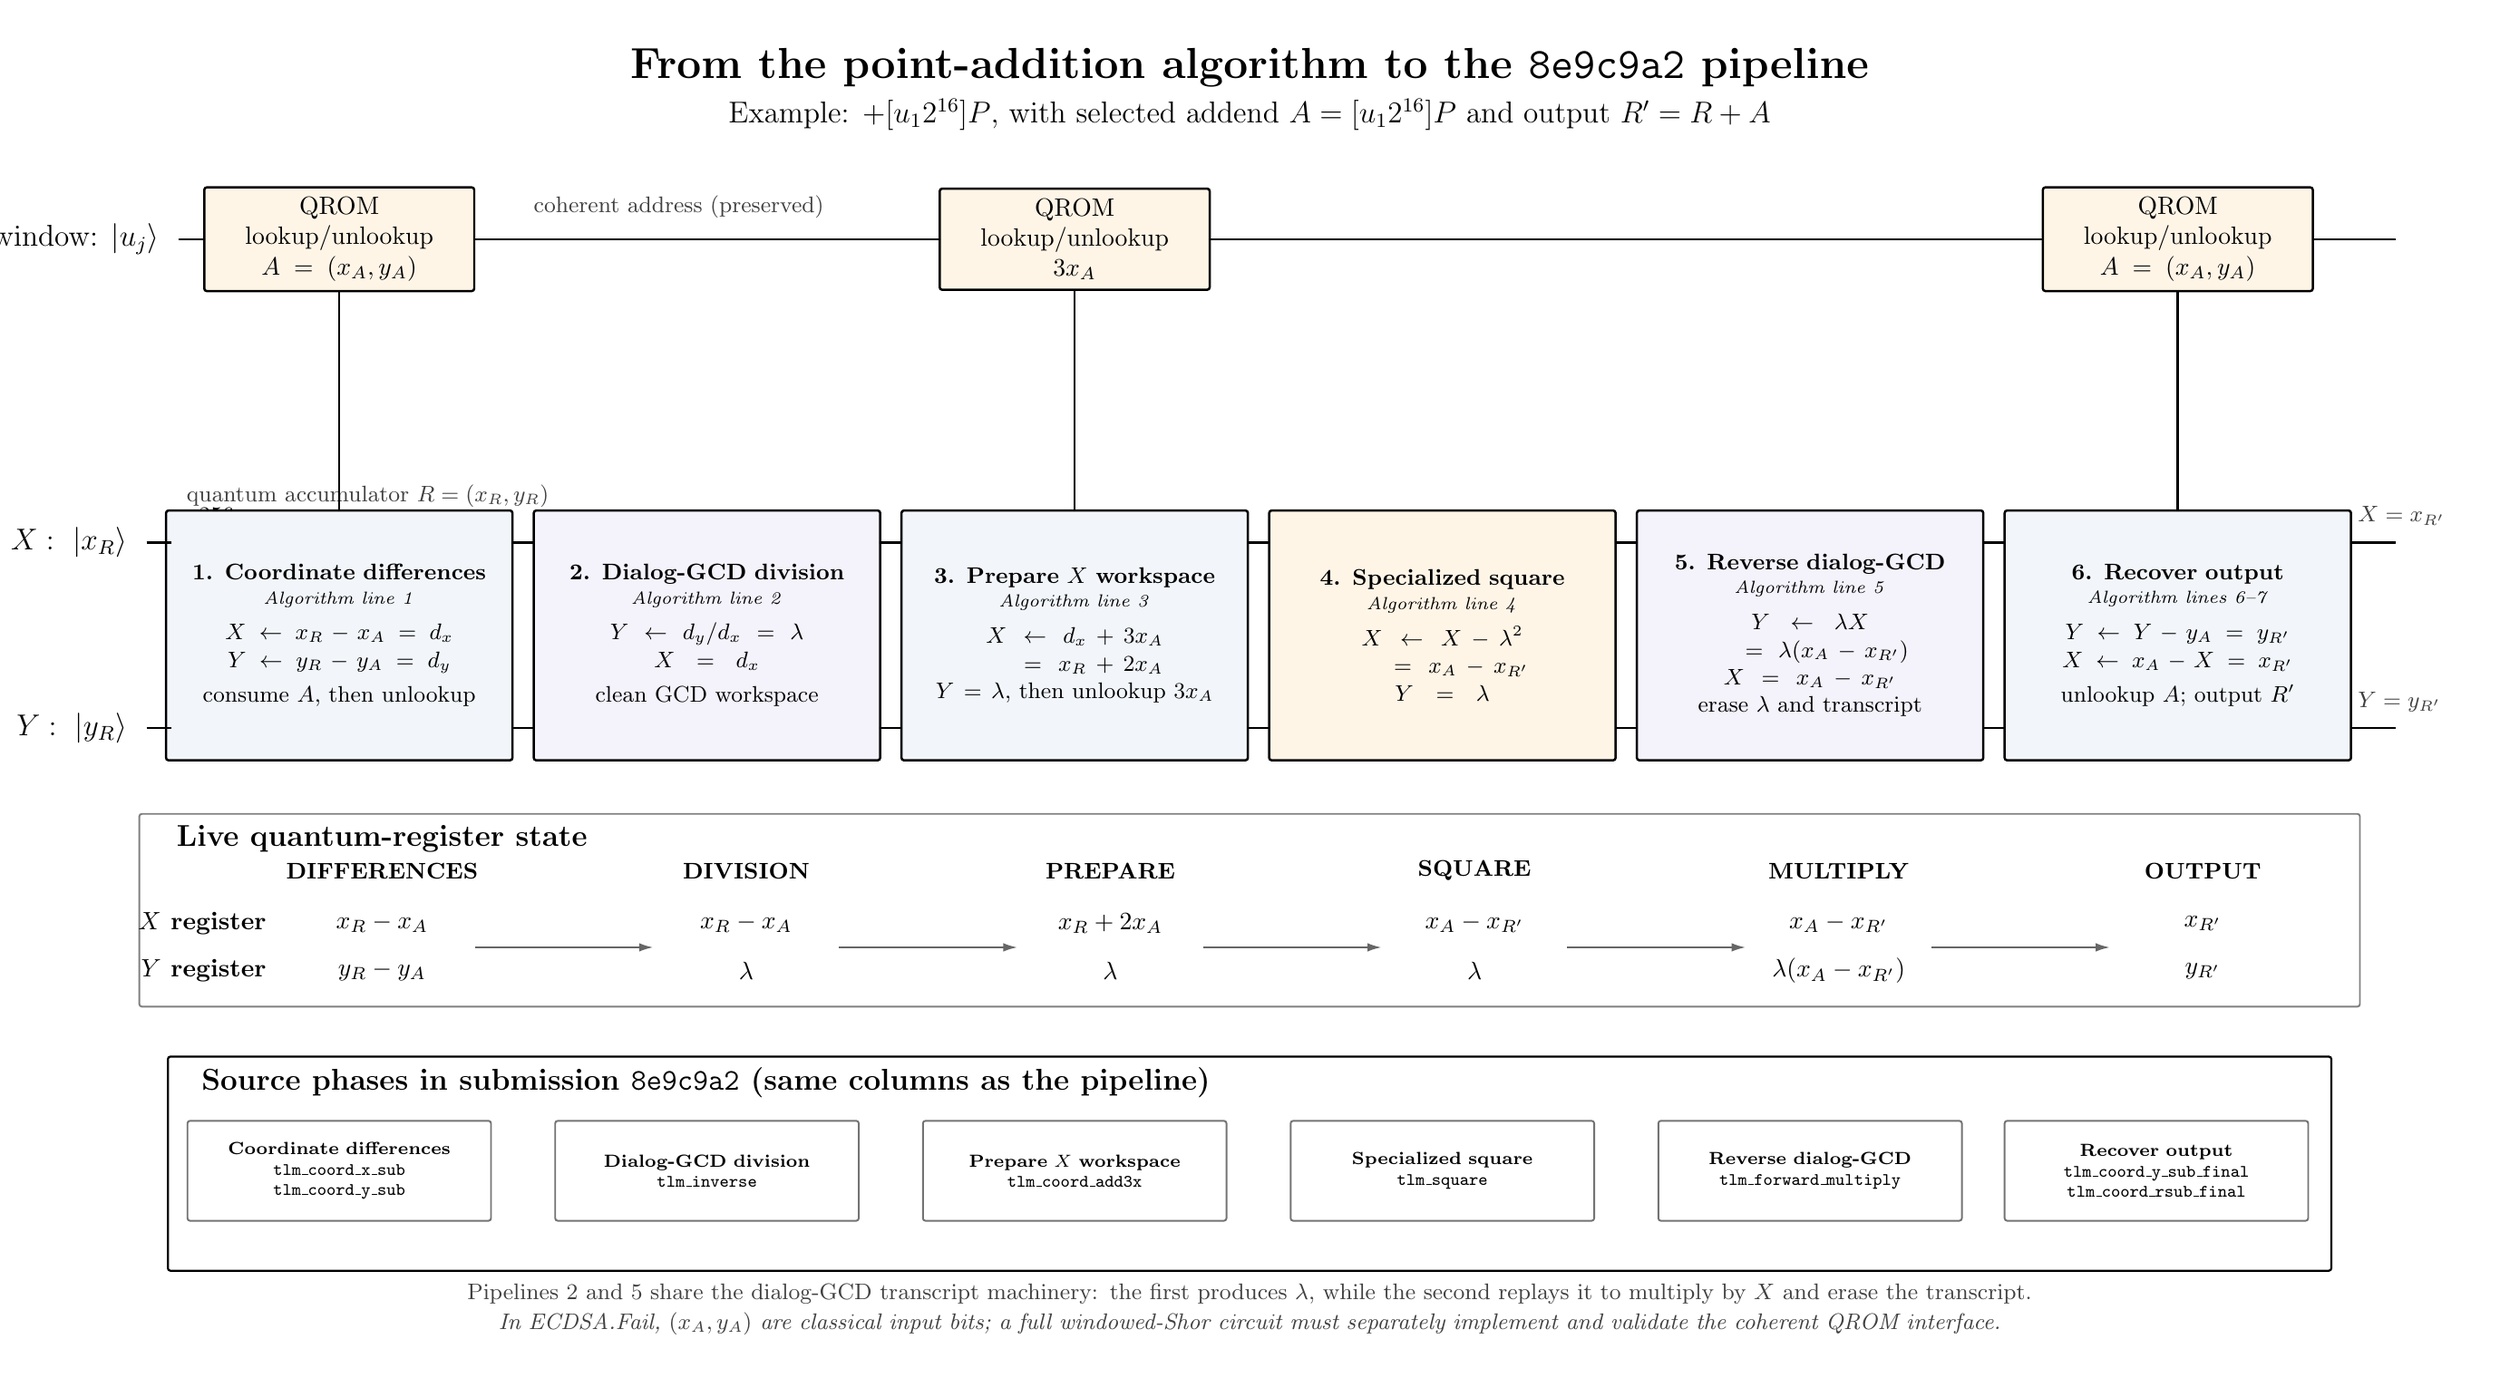
\begin{tikzpicture}[x=1cm,y=1cm]
  \path[use as bounding box] (0,0) rectangle (34.3,18.6);

  \node[font=\LARGE\bfseries] at (17.15,18.0)
    {From the point-addition algorithm to the \texttt{8e9c9a2} pipeline};
  \node[font=\large] at (17.15,17.35)
    {Example: $+[u_1 2^{16}]P$, with selected addend $A=[u_1 2^{16}]P$ and output $R'=R+A$};

  % Window address and three local lookups.
  \node[lab, anchor=east] at (2.0,15.6) {window: $\ket{u_j}$};
  \draw[wire] (2.15,15.6) -- (33.2,15.6);
  \draw[wire] (2.55,15.46) -- (2.82,15.74);
  \node[font=\small] at (2.68,15.98) {$16$};
  \node[note, anchor=west] at (7.0,16.05) {coherent address (preserved)};
  \node[lookup, text width=35mm] (QA) at (4.4,15.6)
    {QROM lookup/unlookup\\$A=(x_A,y_A)$};
  \node[lookup, text width=35mm] (Q3) at (14.7,15.6)
    {QROM lookup/unlookup\\$3x_A$};
  \node[lookup, text width=35mm] (QB) at (30.15,15.6)
    {QROM lookup/unlookup\\$A=(x_A,y_A)$};

  % X and Y coordinate buses.
  \node[lab, anchor=east] at (1.55,11.35) {$X:\ \ket{x_R}$};
  \node[lab, anchor=east] at (1.55,8.75) {$Y:\ \ket{y_R}$};
  \draw[wire] (2.15,11.35) -- (33.2,11.35);
  \draw[wire] (2.15,8.75) -- (33.2,8.75);
  \draw[wire] (2.55,11.21) -- (2.82,11.49);
  \draw[wire] (2.55,8.61) -- (2.82,8.89);
  \node[font=\small] at (2.68,11.73) {$256$};
  \node[font=\small] at (2.68,9.13) {$256$};
  \node[note] at (4.8,12.0) {quantum accumulator $R=(x_R,y_R)$};

  % Six source-level phases.
  \node[phase] (S1) at (4.4,10.05)
    {\textbf{1. Coordinate differences}\\[-0.5mm]
     \textit{\scriptsize Algorithm line 1}\\[1.2mm]
     $X\gets x_R-x_A=d_x$\\
     $Y\gets y_R-y_A=d_y$\\[1mm]
     consume $A$, then unlookup};
  \node[phaseviolet] (S2) at (9.55,10.05)
    {\textbf{2. Dialog-GCD division}\\[-0.5mm]
     \textit{\scriptsize Algorithm line 2}\\[1.2mm]
     $Y\gets d_y/d_x=\lambda$\\
     $X=d_x$\\[1mm]
     clean GCD workspace};
  \node[phase] (S3) at (14.7,10.05)
    {\textbf{3. Prepare $X$ workspace}\\[-0.5mm]
     \textit{\scriptsize Algorithm line 3}\\[1.2mm]
     $X\gets d_x+3x_A$\\
     $\phantom{X}=x_R+2x_A$\\
     $Y=\lambda$, then unlookup $3x_A$};
  \node[phaseorange] (S4) at (19.85,10.05)
    {\textbf{4. Specialized square}\\[-0.5mm]
     \textit{\scriptsize Algorithm line 4}\\[1.2mm]
     $X\gets X-\lambda^2$\\
     $\phantom{X}=x_A-x_{R'}$\\
     $Y=\lambda$};
  \node[phaseviolet] (S5) at (25.0,10.05)
    {\textbf{5. Reverse dialog-GCD}\\[-0.5mm]
     \textit{\scriptsize Algorithm line 5}\\[1.2mm]
     $Y\gets\lambda X$\\
     $\phantom{Y}=\lambda(x_A-x_{R'})$\\
     $X=x_A-x_{R'}$\\
     erase $\lambda$ and transcript};
  \node[phase] (S6) at (30.15,10.05)
    {\textbf{6. Recover output}\\[-0.5mm]
     \textit{\scriptsize Algorithm lines 6--7}\\[1.2mm]
     $Y\gets Y-y_A=y_{R'}$\\
     $X\gets x_A-X=x_{R'}$\\[1mm]
     unlookup $A$; output $R'$};

  % Plain input wires stop at the boundary of the first pipeline stage.
  \draw[wire] (1.70,11.35) -- (2.05,11.35);
  \draw[wire] (1.70,8.75) -- (2.05,8.75);

  \draw[wire] (QA.south) -- (S1.north);
  \draw[wire] (Q3.south) -- (S3.north);
  \draw[wire] (QB.south) -- (S6.north);
  \node[note, anchor=west] at (32.55,11.72) {$X=x_{R'}$};
  \node[note, anchor=west] at (32.55,9.12) {$Y=y_{R'}$};

  % Live-register state table.
  \draw[black!50, line width=0.7pt, rounded corners=1pt]
    (1.6,4.85) rectangle (32.7,7.55);
  \node[font=\large\bfseries, anchor=west] at (2.0,7.2)
    {Live quantum-register state};

  \foreach \xx/\head/\xval/\yval in {
    5.0/DIFFERENCES/{x_R-x_A}/{y_R-y_A},
    10.1/DIVISION/{x_R-x_A}/{\lambda},
    15.2/PREPARE/{x_R+2x_A}/{\lambda},
    20.3/SQUARE/{x_A-x_{R'}}/{\lambda},
    25.4/MULTIPLY/{x_A-x_{R'}}/{\lambda(x_A-x_{R'})},
    30.5/OUTPUT/{x_{R'}}/{y_{R'}}}{
      \node[font=\small\bfseries] at (\xx,6.75) {\head};
      \node[font=\normalsize] at (\xx,6.02) {$\xval$};
      \node[font=\normalsize] at (\xx,5.35) {$\yval$};
  }
  \node[font=\normalsize\bfseries, anchor=east] at (3.5,6.02) {$X$ register};
  \node[font=\normalsize\bfseries, anchor=east] at (3.5,5.35) {$Y$ register};
  \foreach \xa/\xb in {6.3/8.8,11.4/13.9,16.5/19.0,21.6/24.1,26.7/29.2}{
    \draw[flow, black!60] (\xa,5.68) -- (\xb,5.68);
  }

  % Source-level mapping, aligned with the six pipeline columns.
  \draw[black, line width=0.8pt, rounded corners=1pt]
    (2.0,1.15) rectangle (32.3,4.15);
  \node[font=\large\bfseries, anchor=west] at (2.35,3.78)
    {Source phases in submission \texttt{8e9c9a2} (same columns as the pipeline)};
  \node[registerbox, text width=39mm, minimum height=14mm, font=\scriptsize] at (4.4,2.55)
    {\textbf{Coordinate differences}\\
     \texttt{tlm\_coord\_x\_sub}\\
     \texttt{tlm\_coord\_y\_sub}};
  \node[registerbox, text width=39mm, minimum height=14mm, font=\scriptsize] at (9.55,2.55)
    {\textbf{Dialog-GCD division}\\
     \texttt{tlm\_inverse}};
  \node[registerbox, text width=39mm, minimum height=14mm, font=\scriptsize] at (14.7,2.55)
    {\textbf{Prepare $X$ workspace}\\
     \texttt{tlm\_coord\_add3x}};
  \node[registerbox, text width=39mm, minimum height=14mm, font=\scriptsize] at (19.85,2.55)
    {\textbf{Specialized square}\\
     \texttt{tlm\_square}};
  \node[registerbox, text width=39mm, minimum height=14mm, font=\scriptsize] at (25.0,2.55)
    {\textbf{Reverse dialog-GCD}\\
     \texttt{tlm\_forward\_multiply}};
  \node[registerbox, text width=39mm, minimum height=14mm, font=\scriptsize] at (29.85,2.55)
    {\textbf{Recover output}\\
     \texttt{tlm\_coord\_y\_sub\_final}\\
     \texttt{tlm\_coord\_rsub\_final}};

  \node[note, text width=31cm, align=center] at (17.15,0.82)
    {Pipelines 2 and 5 share the dialog-GCD transcript machinery: the first produces $\lambda$, while the second replays it to multiply by $X$ and erase the transcript.};
  \node[note, text width=31cm, align=center, font=\small\itshape] at (17.15,0.40)
    {In ECDSA.Fail, $(x_A,y_A)$ are classical input bits; a full windowed-Shor circuit must separately implement and validate the coherent QROM interface.};
\end{tikzpicture}

\newpage

% ============================================================================
% Page 4: phase 1, coordinate differences
% ============================================================================
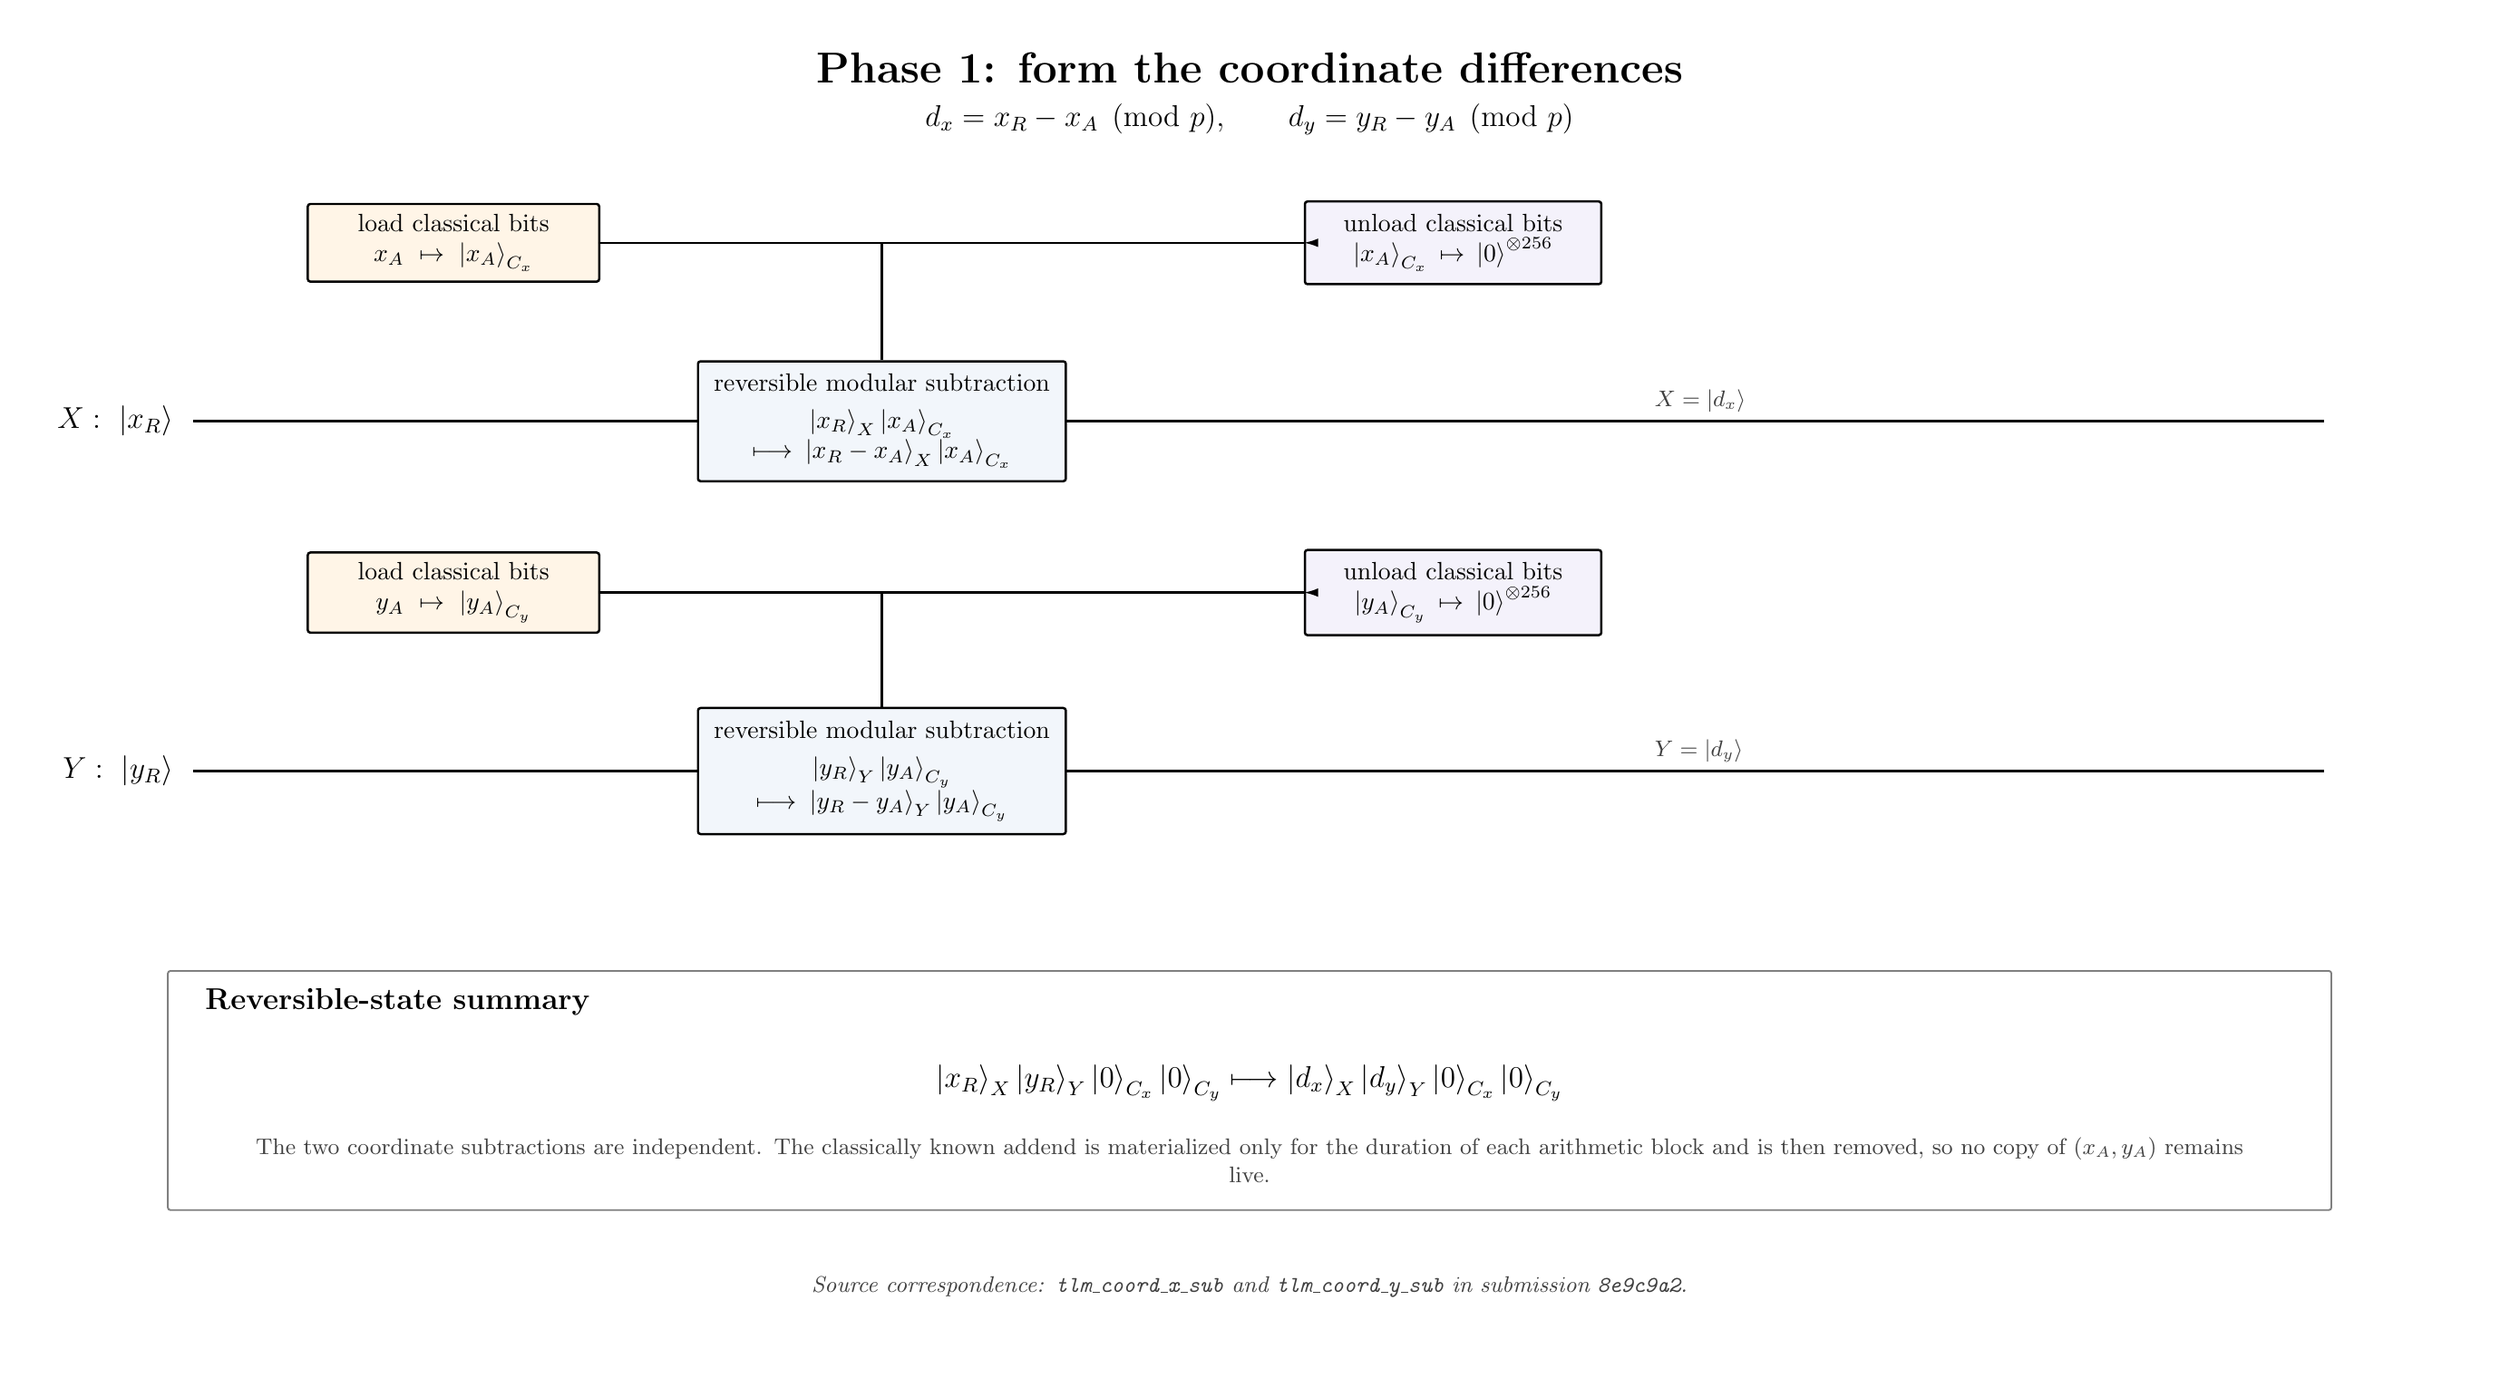
\begin{tikzpicture}[x=1cm,y=1cm]
  \path[use as bounding box] (0,0) rectangle (34.3,18.6);

  \node[font=\LARGE\bfseries] at (17.15,18.0)
    {Phase 1: form the coordinate differences};
  \node[font=\large] at (17.15,17.28)
    {$d_x=x_R-x_A\pmod p,\qquad d_y=y_R-y_A\pmod p$};

  % X lane and its classical addend workspace.
  \node[lab, anchor=east] at (2.2,13.05) {$X:\ \ket{x_R}$};
  \draw[wire] (2.35,13.05) -- (32.2,13.05);
  \node[lookup, text width=38mm] (LX) at (6.0,15.55)
    {load classical bits\\$x_A\mapsto\ket{x_A}_{C_x}$};
  \draw[wire] (LX.east) -- (18.0,15.55);
  \node[detail, text width=48mm] (SUBX) at (12.0,13.05)
    {reversible modular subtraction\\[1mm]
     $\ket{x_R}_X\ket{x_A}_{C_x}$\\
     $\longmapsto\ket{x_R-x_A}_X\ket{x_A}_{C_x}$};
  \draw[wire] (12.0,15.55) -- (SUBX.north);
  \node[detailviolet, text width=38mm, minimum height=8mm] (UX) at (20.0,15.55)
    {unload classical bits\\$\ket{x_A}_{C_x}\mapsto\ket{0}^{\otimes256}$};
  \draw[flow] (18.0,15.55) -- (UX.west);
  \node[note, anchor=south west] at (22.7,13.05) {$X=\ket{d_x}$};

  % Y lane and its classical addend workspace.
  \node[lab, anchor=east] at (2.2,8.15) {$Y:\ \ket{y_R}$};
  \draw[wire] (2.35,8.15) -- (32.2,8.15);
  \node[lookup, text width=38mm] (LY) at (6.0,10.65)
    {load classical bits\\$y_A\mapsto\ket{y_A}_{C_y}$};
  \draw[wire] (LY.east) -- (18.0,10.65);
  \node[detail, text width=48mm] (SUBY) at (12.0,8.15)
    {reversible modular subtraction\\[1mm]
     $\ket{y_R}_Y\ket{y_A}_{C_y}$\\
     $\longmapsto\ket{y_R-y_A}_Y\ket{y_A}_{C_y}$};
  \draw[wire] (12.0,10.65) -- (SUBY.north);
  \node[detailviolet, text width=38mm, minimum height=8mm] (UY) at (20.0,10.65)
    {unload classical bits\\$\ket{y_A}_{C_y}\mapsto\ket{0}^{\otimes256}$};
  \draw[flow] (18.0,10.65) -- (UY.west);
  \node[note, anchor=south west] at (22.7,8.15) {$Y=\ket{d_y}$};

  \draw[black!50, line width=0.7pt, rounded corners=1pt]
    (2.0,2.0) rectangle (32.3,5.35);
  \node[font=\large\bfseries, anchor=west] at (2.4,4.92)
    {Reversible-state summary};
  \node[font=\large] at (17.15,3.78)
    {$\ket{x_R}_X\ket{y_R}_Y\ket{0}_{C_x}\ket{0}_{C_y}
      \longmapsto
      \ket{d_x}_X\ket{d_y}_Y\ket{0}_{C_x}\ket{0}_{C_y}$};
  \node[note, text width=28cm, align=center] at (17.15,2.70)
    {The two coordinate subtractions are independent.  The classically known addend is materialized only for the duration of each arithmetic block and is then removed, so no copy of $(x_A,y_A)$ remains live.};
  \node[note, text width=29cm, align=center, font=\small\itshape] at (17.15,0.92)
    {Source correspondence: \texttt{tlm\_coord\_x\_sub} and \texttt{tlm\_coord\_y\_sub} in submission \texttt{8e9c9a2}.};
\end{tikzpicture}

\newpage

% ============================================================================
% Page 5: phase 1 implementation details
% ============================================================================
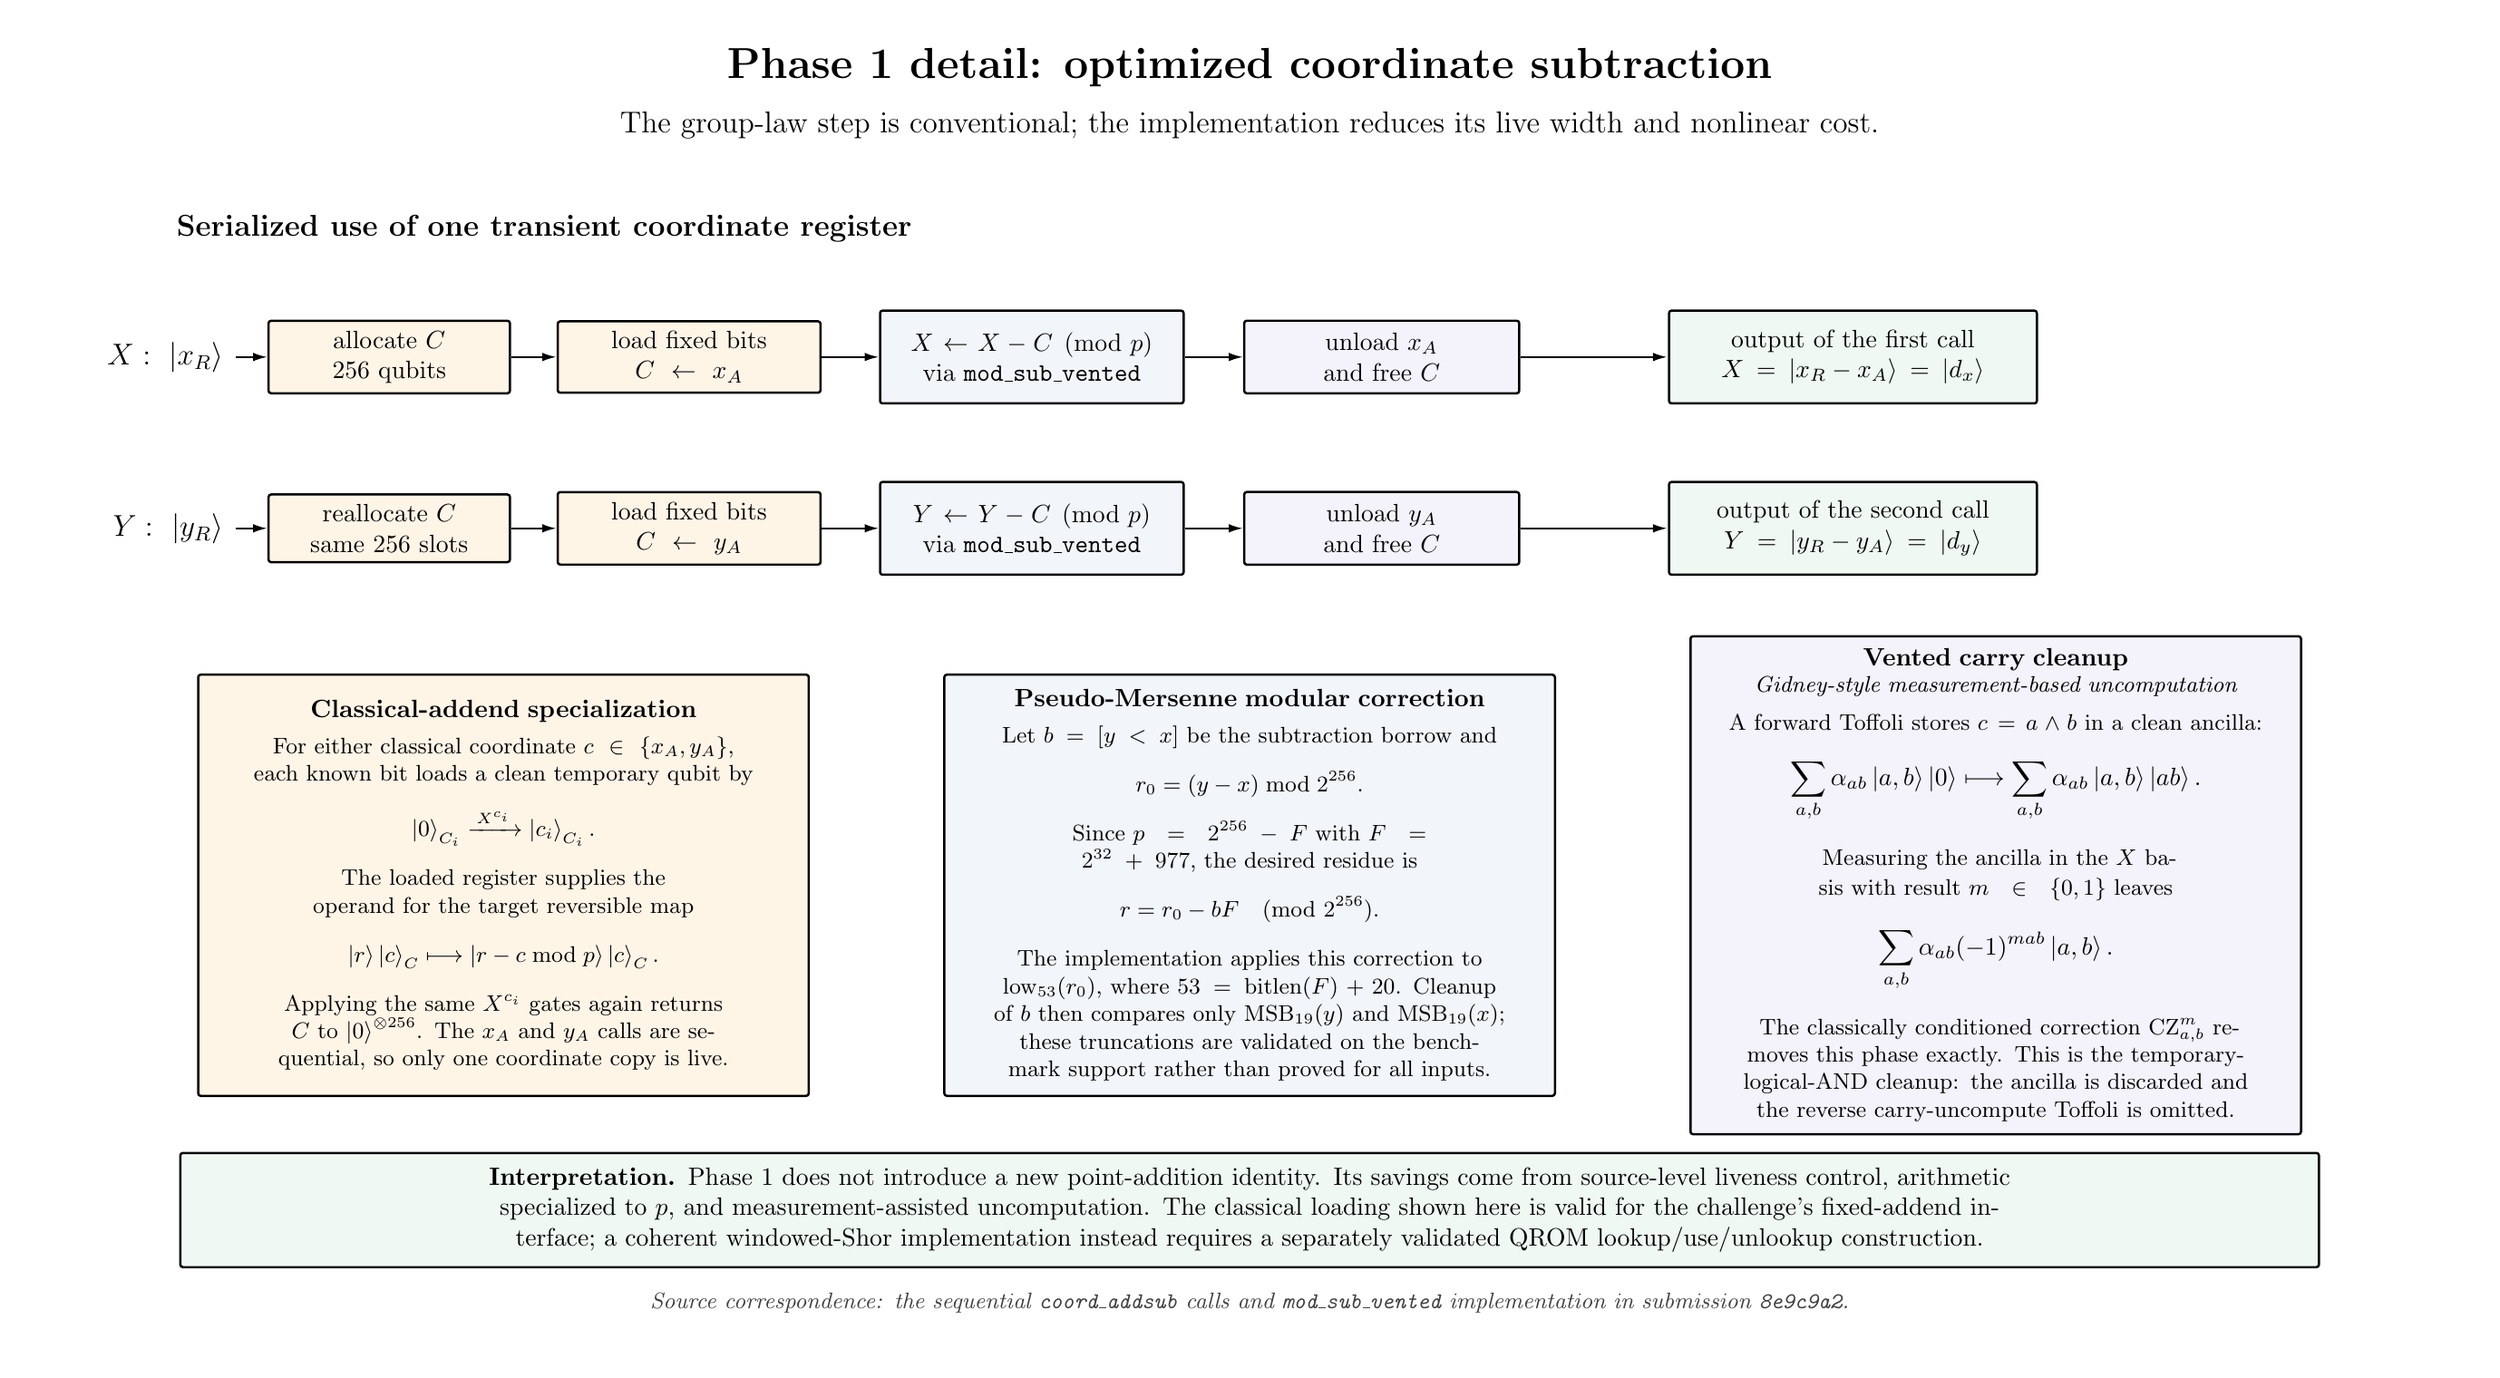
\begin{tikzpicture}[x=1cm,y=1cm]
  \path[use as bounding box] (0,0) rectangle (34.3,18.6);

  \node[font=\LARGE\bfseries] at (17.15,18.0)
    {Phase 1 detail: optimized coordinate subtraction};
  \node[font=\large] at (17.15,17.20)
    {The group-law step is conventional; the implementation reduces its live width and nonlinear cost.};

  % The two source-level calls execute sequentially and reuse the same temporary register.
  \node[font=\large\bfseries, anchor=west] at (2.0,15.75)
    {Serialized use of one transient coordinate register};

  \node[lab, anchor=east] at (2.9,13.95) {$X:\ \ket{x_R}$};
  \node[lookup, text width=31mm] (LX1) at (5.1,13.95)
    {allocate $C$\\$256$ qubits};
  \node[lookup, text width=34mm] (LX2) at (9.3,13.95)
    {load fixed bits\\$C\gets x_A$};
  \node[detail, text width=39mm, minimum height=13mm] (LX3) at (14.1,13.95)
    {$X\gets X-C\pmod p$\\via \texttt{mod\_sub\_vented}};
  \node[detailviolet, text width=35mm, minimum height=8mm] (LX4) at (19.0,13.95)
    {unload $x_A$\\and free $C$};
  \draw[flow] (2.95,13.95) -- (LX1.west);
  \draw[flow] (LX1.east) -- (LX2.west);
  \draw[flow] (LX2.east) -- (LX3.west);
  \draw[flow] (LX3.east) -- (LX4.west);
  \node[detailgreen, text width=48mm, minimum height=13mm] at (25.6,13.95)
    {output of the first call\\$X=\ket{x_R-x_A}=\ket{d_x}$};
  \draw[flow] (LX4.east) -- (23.0,13.95);

  \node[lab, anchor=east] at (2.9,11.55) {$Y:\ \ket{y_R}$};
  \node[lookup, text width=31mm] (LY1) at (5.1,11.55)
    {reallocate $C$\\same $256$ slots};
  \node[lookup, text width=34mm] (LY2) at (9.3,11.55)
    {load fixed bits\\$C\gets y_A$};
  \node[detail, text width=39mm, minimum height=13mm] (LY3) at (14.1,11.55)
    {$Y\gets Y-C\pmod p$\\via \texttt{mod\_sub\_vented}};
  \node[detailviolet, text width=35mm, minimum height=8mm] (LY4) at (19.0,11.55)
    {unload $y_A$\\and free $C$};
  \draw[flow] (2.95,11.55) -- (LY1.west);
  \draw[flow] (LY1.east) -- (LY2.west);
  \draw[flow] (LY2.east) -- (LY3.west);
  \draw[flow] (LY3.east) -- (LY4.west);
  \node[detailgreen, text width=48mm, minimum height=13mm] at (25.6,11.55)
    {output of the second call\\$Y=\ket{y_R-y_A}=\ket{d_y}$};
  \draw[flow] (LY4.east) -- (23.0,11.55);

  % Three implementation mechanisms.
  \node[detailorange, text width=82mm, minimum height=59mm, font=\small] (C1) at (6.7,6.55)
    {{\normalsize\bfseries Classical-addend specialization}\\[1.2mm]
     For either classical coordinate $c\in\{x_A,y_A\}$, each known bit loads a clean temporary qubit by
     \[
       \ket{0}_{C_i}\xrightarrow{\,X^{c_i}\,}\ket{c_i}_{C_i}.
     \]
     The loaded register supplies the operand for the target reversible map
     \[
       \ket{r}\ket{c}_C\longmapsto
       \ket{r-c\bmod p}\ket{c}_C.
     \]
     Applying the same $X^{c_i}$ gates again returns $C$ to $\ket{0}^{\otimes256}$. The $x_A$ and $y_A$ calls are sequential, so only one coordinate copy is live.};

  \node[detail, text width=82mm, minimum height=59mm, font=\small] (C2) at (17.15,6.55)
    {{\normalsize\bfseries Pseudo-Mersenne modular correction}\\[1.2mm]
     Let $b=[y<x]$ be the subtraction borrow and
     \[
       r_0=(y-x)\bmod 2^{256}.
     \]
     Since $p=2^{256}-F$ with $F=2^{32}+977$, the desired residue is
     \[
       r=r_0-bF\pmod{2^{256}}.
     \]
     The implementation applies this correction to
     $\operatorname{low}_{53}(r_0)$, where $53=\operatorname{bitlen}(F)+20$.
     Cleanup of $b$ then compares only
     $\operatorname{MSB}_{19}(y)$ and $\operatorname{MSB}_{19}(x)$; these truncations are validated on the benchmark support rather than proved for all inputs.};

  \node[detailviolet, text width=82mm, minimum height=59mm, font=\small] (C3) at (27.6,6.55)
    {{\normalsize\bfseries Vented carry cleanup}\\[-0.3mm]
     {\itshape Gidney-style measurement-based uncomputation}\\[1.2mm]
     A forward Toffoli stores $c=a\wedge b$ in a clean ancilla:
     {\normalsize
     \[
       \sum_{a,b}\alpha_{ab}\ket{a,b}\ket{0}
       \longmapsto
       \sum_{a,b}\alpha_{ab}\ket{a,b}\ket{ab}.
     \]}
     Measuring the ancilla in the $X$ basis with result $m\in\{0,1\}$ leaves
     {\normalsize
     \[
       \sum_{a,b}\alpha_{ab}(-1)^{mab}\ket{a,b}.
     \]}
     The classically conditioned correction $\mathrm{CZ}^{m}_{a,b}$ removes this phase exactly. This is the temporary-logical-AND cleanup: the ancilla is discarded and the reverse carry-uncompute Toffoli is omitted.};

  \node[detailgreen, text width=296mm, minimum height=16mm] at (17.15,2.0)
    {\textbf{Interpretation.} Phase 1 does not introduce a new point-addition identity. Its savings come from source-level liveness control, arithmetic specialized to $p$, and measurement-assisted uncomputation. The classical loading shown here is valid for the challenge's fixed-addend interface; a coherent windowed-Shor implementation instead requires a separately validated QROM lookup/use/unlookup construction.};

  \node[note, text width=29cm, align=center, font=\small\itshape] at (17.15,0.70)
    {Source correspondence: the sequential \texttt{coord\_addsub} calls and \texttt{mod\_sub\_vented} implementation in submission \texttt{8e9c9a2}.};
\end{tikzpicture}

\newpage

% ============================================================================
% Page 6: phase 2, dialog-GCD division
% ============================================================================
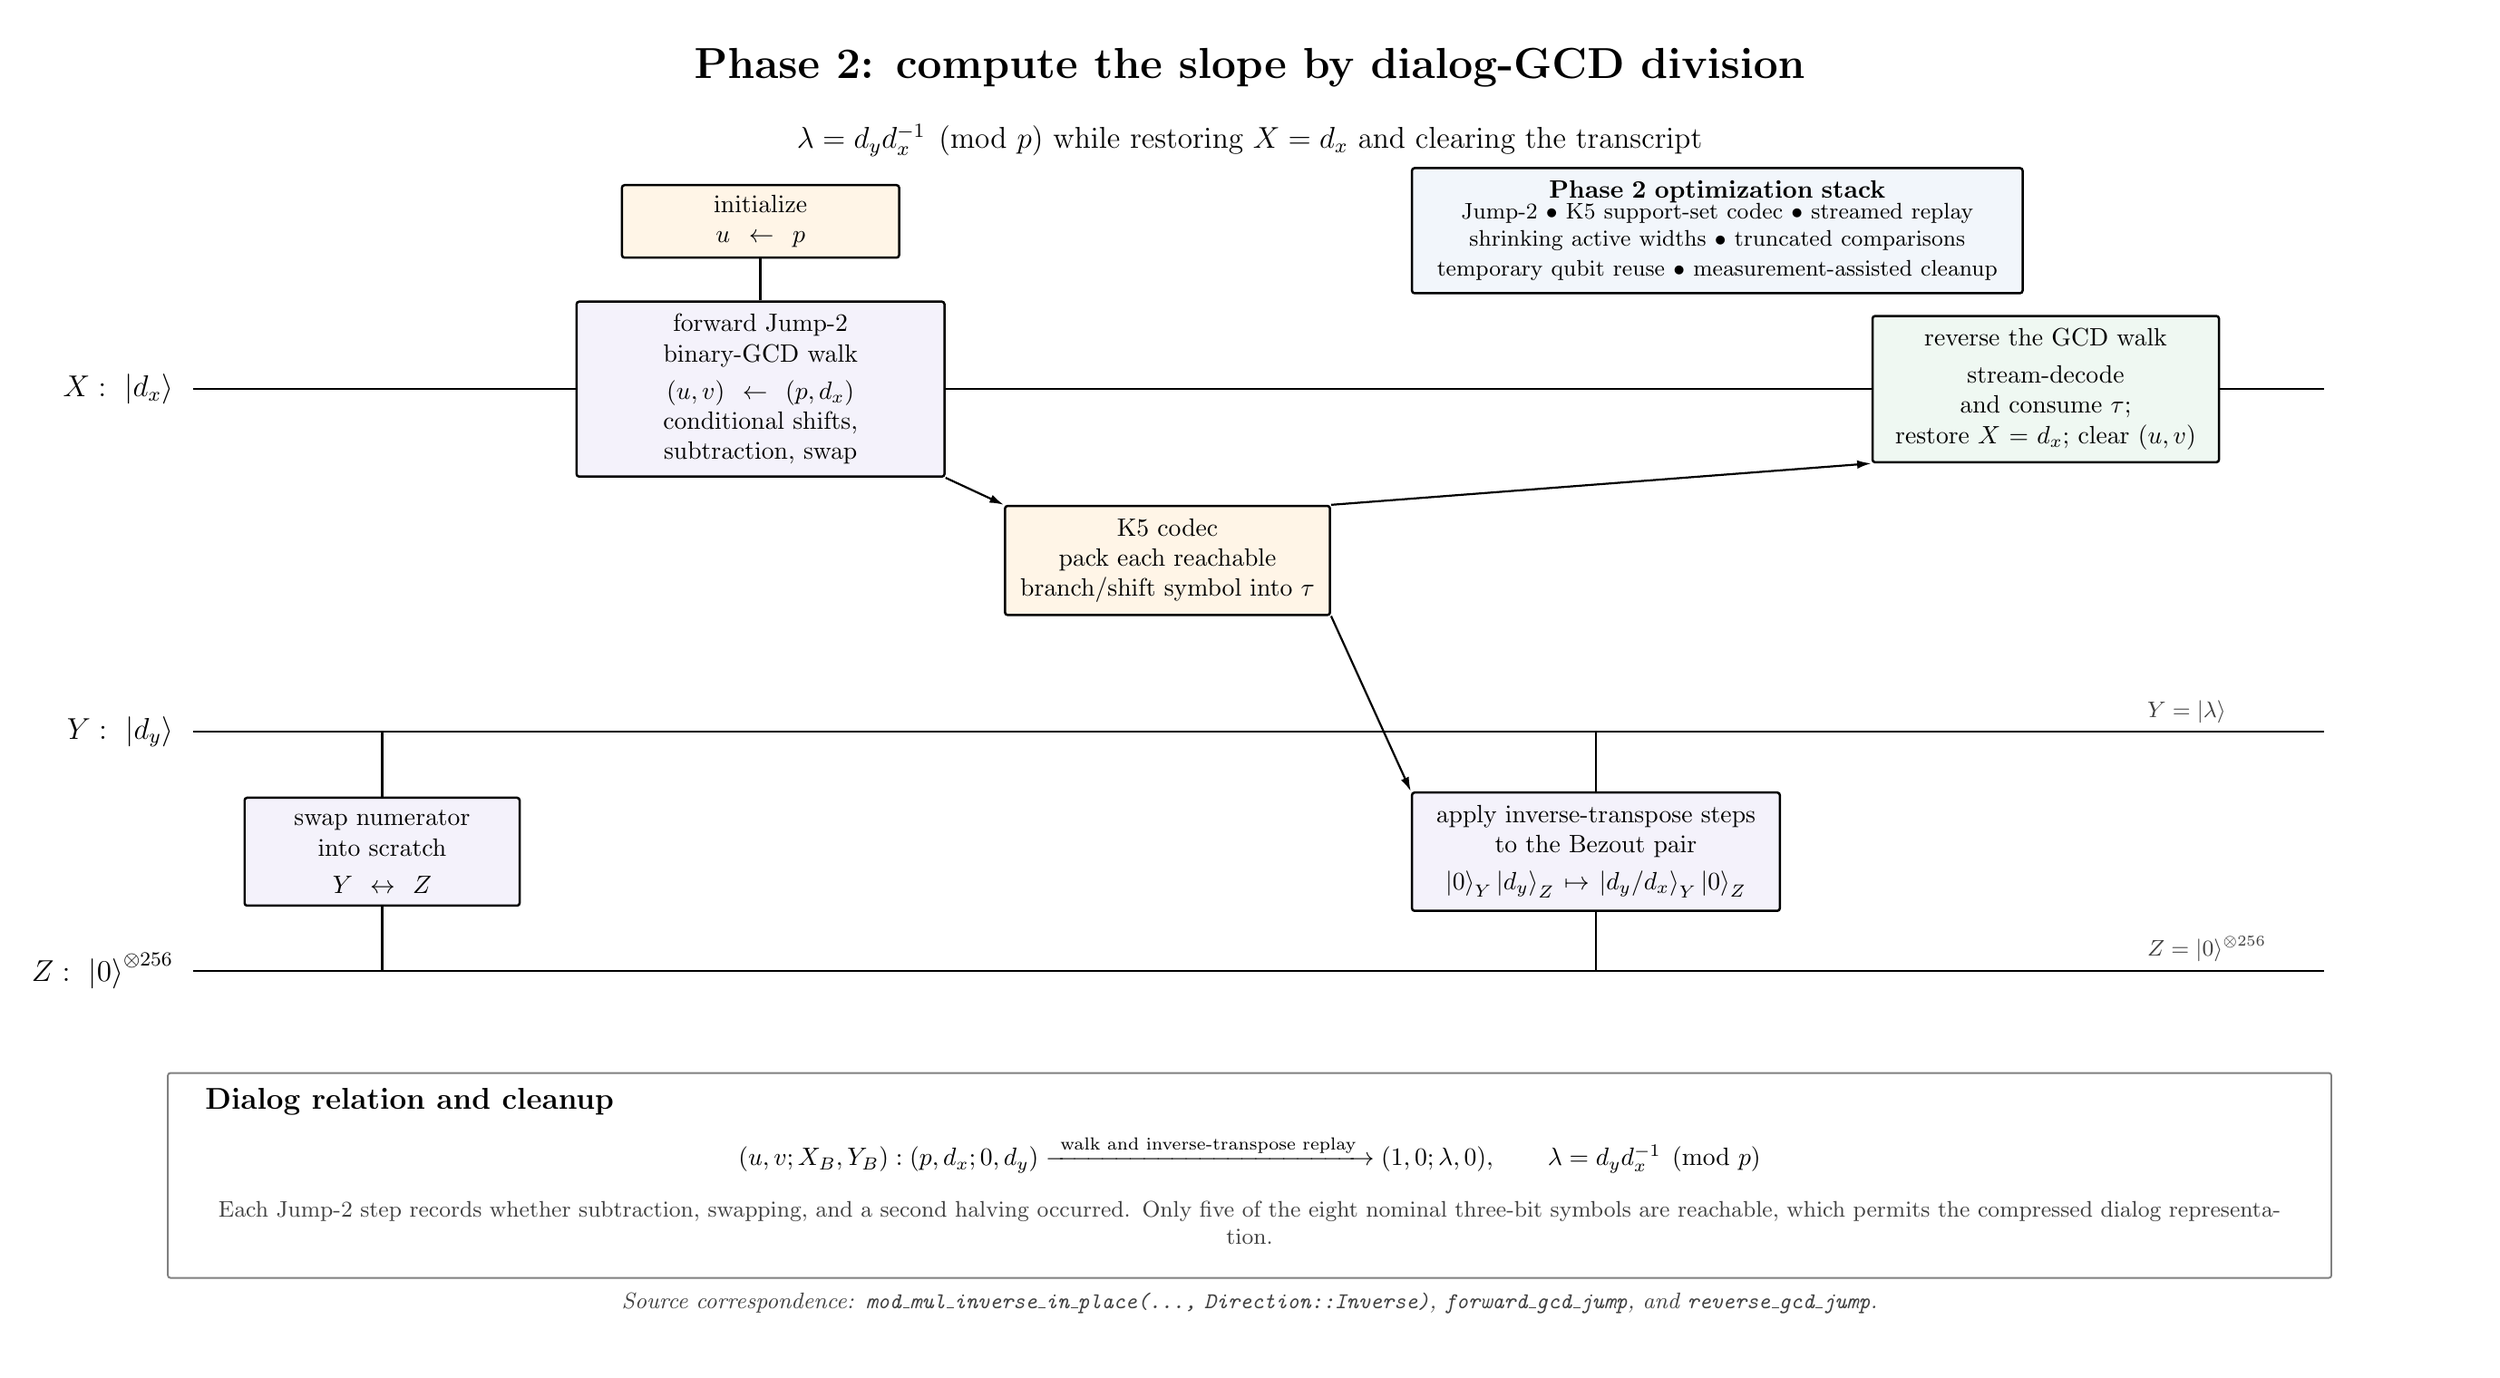
\begin{tikzpicture}[x=1cm,y=1cm]
  \path[use as bounding box] (0,0) rectangle (34.3,18.6);

  \node[font=\LARGE\bfseries] at (17.15,18.0)
    {Phase 2: compute the slope by dialog-GCD division};
  \node[font=\large] at (17.15,16.98)
    {$\lambda=d_y d_x^{-1}\pmod p$ while restoring $X=d_x$ and clearing the transcript};

  \node[lab, anchor=east] at (2.2,13.5) {$X:\ \ket{d_x}$};
  \node[lab, anchor=east] at (2.2,8.7) {$Y:\ \ket{d_y}$};
  \node[lab, anchor=east] at (2.2,5.35) {$Z:\ \ket{0}^{\otimes256}$};
  \draw[wire] (2.35,13.5) -- (32.2,13.5);
  \draw[wire] (2.35,8.7) -- (32.2,8.7);
  \draw[wire] (2.35,5.35) -- (32.2,5.35);

  \node[detailviolet, text width=35mm] (SW) at (5.0,7.02)
    {swap numerator\\into scratch\\[1mm]
     $Y\leftrightarrow Z$};
  \draw[wire] (5.0,8.7) -- (SW.north);
  \draw[wire] (5.0,5.35) -- (SW.south);

  \node[detailviolet, text width=48mm] (WALK) at (10.3,13.5)
    {forward Jump-2 binary-GCD walk\\[1mm]
     $(u,v)\gets(p,d_x)$\\
     conditional shifts, subtraction, swap};
  \node[lookup, text width=36mm] (PREG) at (10.3,15.85)
    {initialize\\$u\gets p$};
  \draw[wire] (PREG.south) -- (WALK.north);

  \node[detailorange, text width=42mm] (TAPE) at (16.0,11.1)
    {K5 codec\\pack each reachable\\branch/shift symbol into $\tau$};
  \draw[flow] (WALK.south east) -- (TAPE.north west);

  \node[detailviolet, text width=48mm] (APPLY) at (22.0,7.02)
    {apply inverse-transpose steps\\to the Bezout pair\\[1mm]
     $\ket{0}_Y\ket{d_y}_Z\mapsto
      \ket{d_y/d_x}_Y\ket{0}_Z$};
  \draw[flow] (TAPE.south east) -- (APPLY.north west);
  \draw[wire] (22.0,8.7) -- (APPLY.north);
  \draw[wire] (22.0,5.35) -- (APPLY.south);

  \node[detailgreen, text width=45mm] (REV) at (28.3,13.5)
    {reverse the GCD walk\\[1mm]
     stream-decode and consume $\tau$;\\
     restore $X=d_x$; clear $(u,v)$};
  \draw[flow] (TAPE.north east) -- (REV.south west);

  \node[detail, text width=82mm, minimum height=14mm] at (23.7,15.72)
    {\textbf{Phase 2 optimization stack}\\[-1mm]
     {\small Jump-2 $\bullet$ K5 support-set codec $\bullet$ streamed replay\\
     shrinking active widths $\bullet$ truncated comparisons\\
     temporary qubit reuse $\bullet$ measurement-assisted cleanup}};

  \node[note, anchor=south west] at (29.6,8.7) {$Y=\ket{\lambda}$};
  \node[note, anchor=south west] at (29.6,5.35) {$Z=\ket{0}^{\otimes256}$};

  \draw[black!50, line width=0.7pt, rounded corners=1pt]
    (2.0,1.05) rectangle (32.3,3.92);
  \node[font=\large\bfseries, anchor=west] at (2.4,3.52)
    {Dialog relation and cleanup};
  \node[font=\normalsize] at (17.15,2.78)
    {$(u,v;X_B,Y_B):(p,d_x;0,d_y)
      \xrightarrow{\ \text{walk and inverse-transpose replay}\ }
      (1,0;\lambda,0),\qquad \lambda=d_y d_x^{-1}\pmod p$};
  \node[note, text width=29cm, align=center] at (17.15,1.82)
    {Each Jump-2 step records whether subtraction, swapping, and a second halving occurred.  Only five of the eight nominal three-bit symbols are reachable, which permits the compressed dialog representation.};
  \node[note, text width=29cm, align=center, font=\small\itshape] at (17.15,0.70)
    {Source correspondence: \texttt{mod\_mul\_inverse\_in\_place(..., Direction::Inverse)}, \texttt{forward\_gcd\_jump}, and \texttt{reverse\_gcd\_jump}.};
\end{tikzpicture}

\newpage

% ============================================================================
% Page 7: Jump-2 step used inside phase 2
% ============================================================================
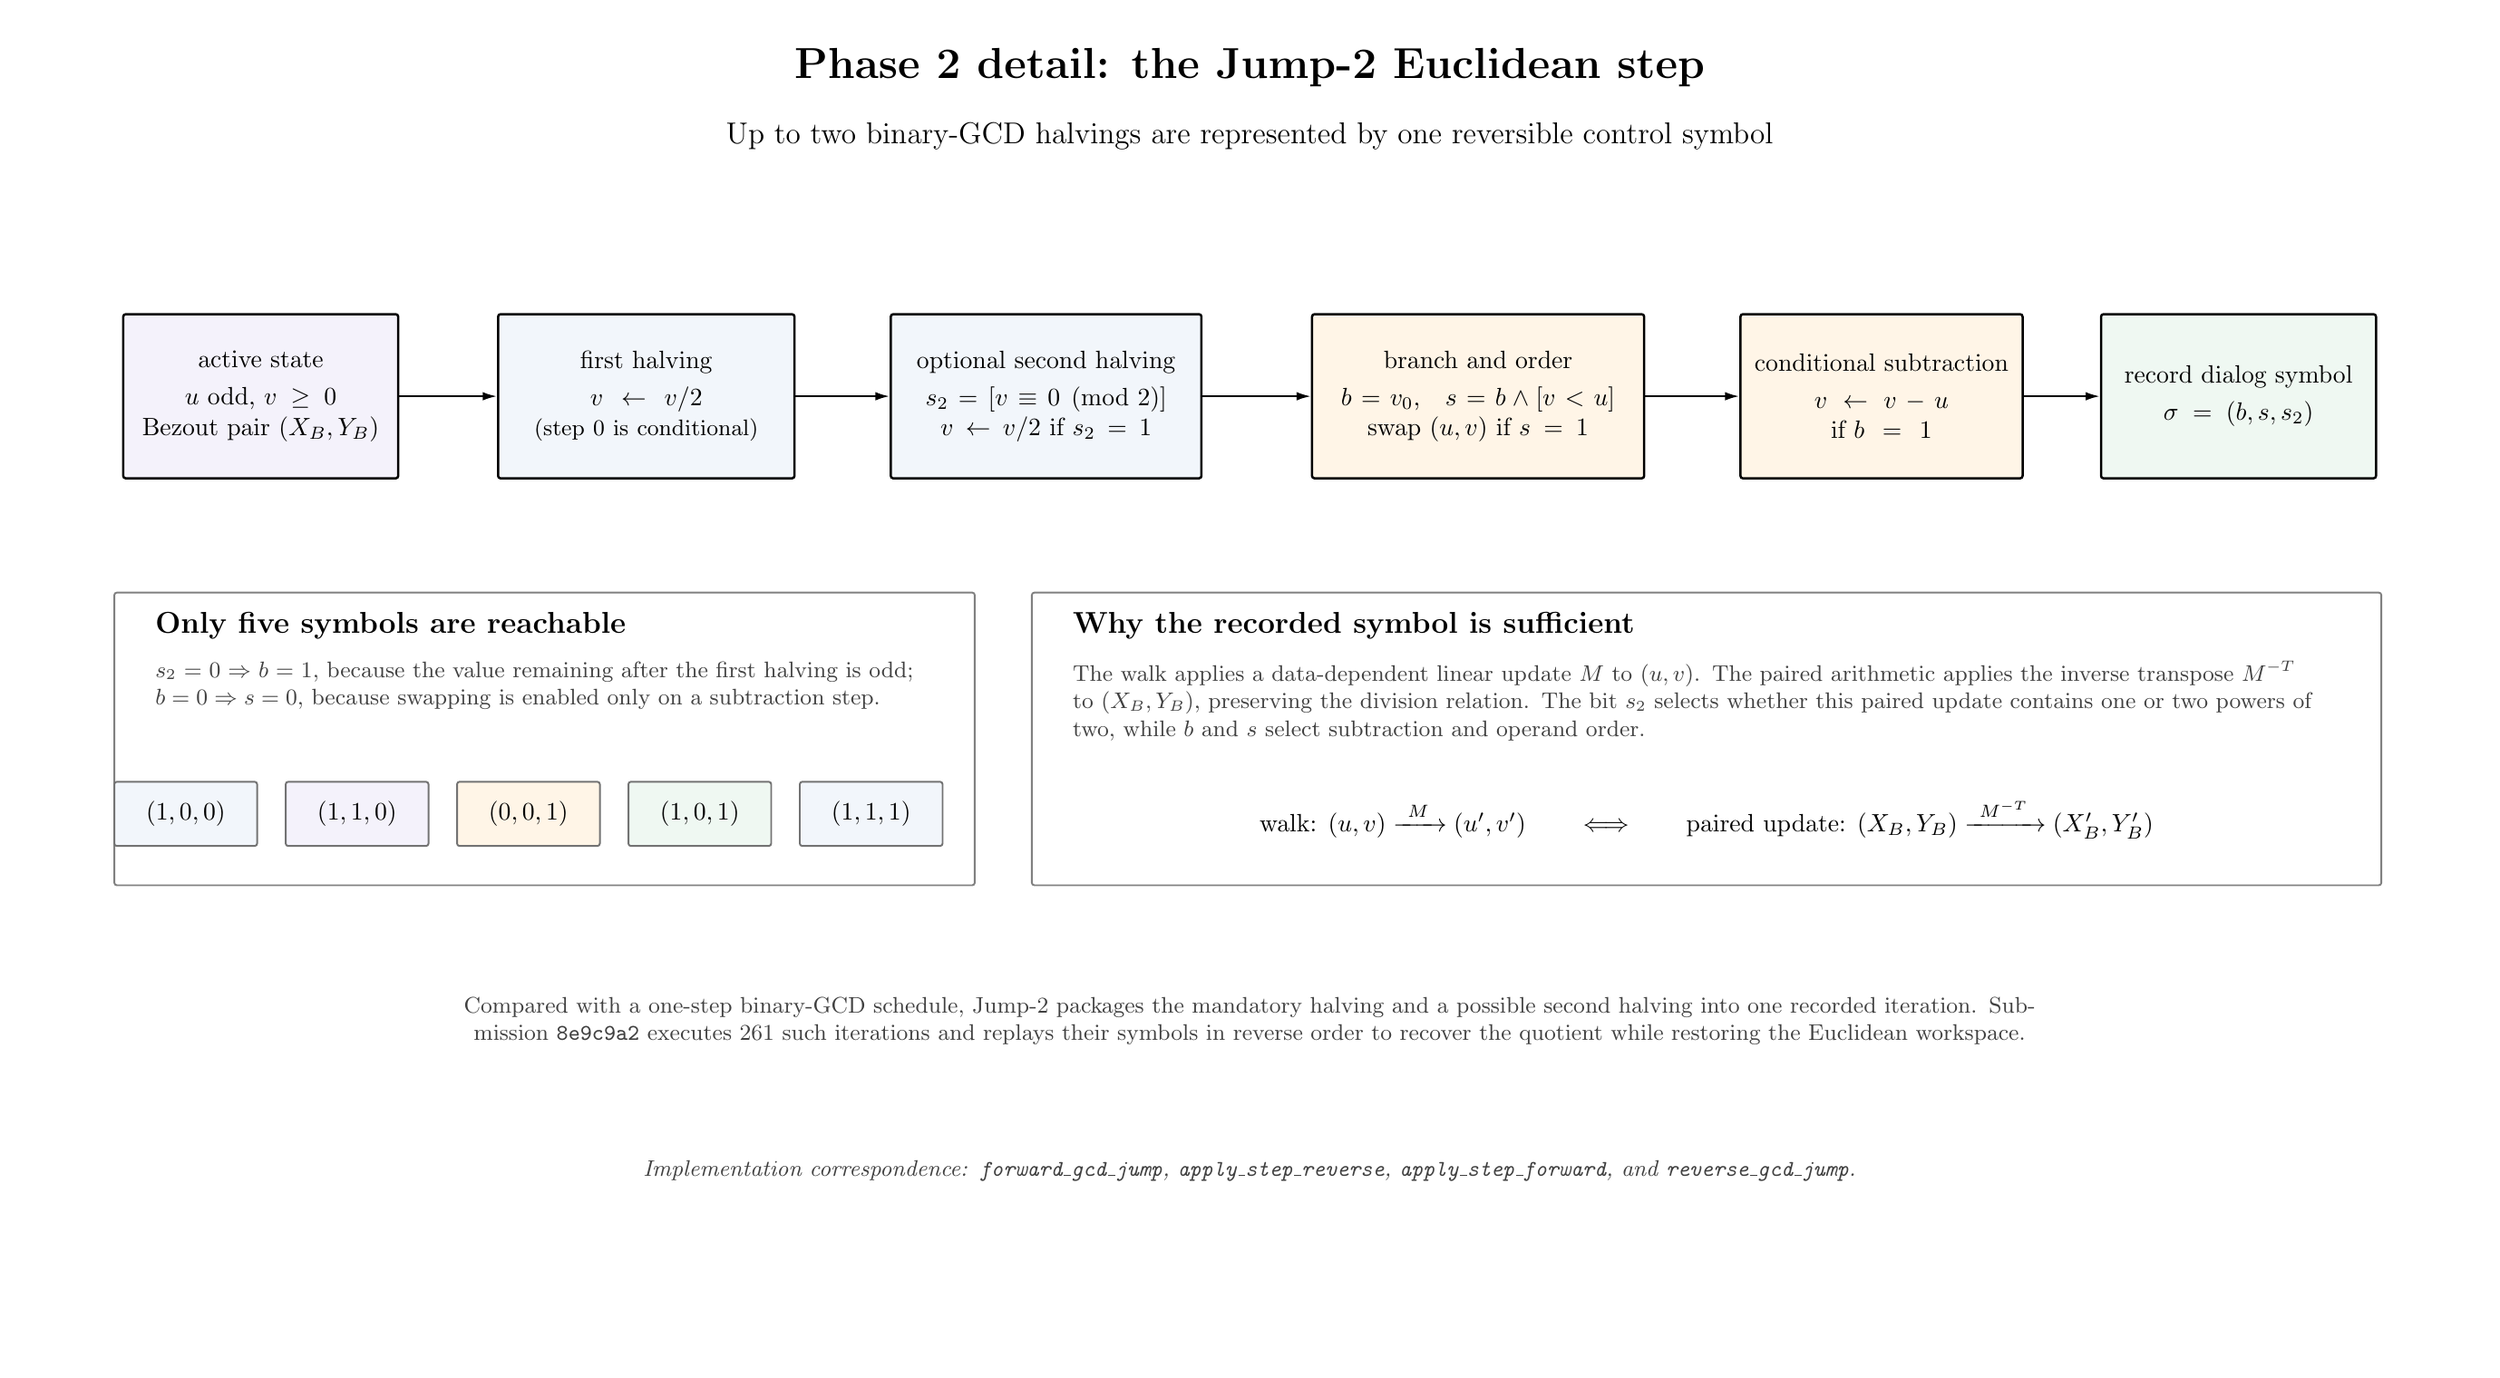
\begin{tikzpicture}[x=1cm,y=1cm]
  \path[use as bounding box] (0,0) rectangle (34.3,18.6);

  \node[font=\LARGE\bfseries] at (17.15,18.0)
    {Phase 2 detail: the Jump-2 Euclidean step};
  \node[font=\large] at (17.15,17.05)
    {Up to two binary-GCD halvings are represented by one reversible control symbol};

  \node[detailviolet, text width=35mm, minimum height=23mm] (S0) at (3.3,13.4)
    {active state\\[1mm]
     $u$ odd, $v\geq0$\\
     Bezout pair $(X_B,Y_B)$};
  \node[detail, text width=38mm, minimum height=23mm] (S1) at (8.7,13.4)
    {first halving\\[1mm]
     $v\leftarrow v/2$\\
     {\small(step $0$ is conditional)}};
  \node[detail, text width=40mm, minimum height=23mm] (S2) at (14.3,13.4)
    {optional second halving\\[1mm]
     $s_2=[v\equiv0\pmod2]$\\
     $v\leftarrow v/2$ if $s_2=1$};
  \node[detailorange, text width=43mm, minimum height=23mm] (S3) at (20.35,13.4)
    {branch and order\\[1mm]
     $b=v_0$,\quad $s=b\wedge[v<u]$\\
     swap $(u,v)$ if $s=1$};
  \node[detailorange, text width=36mm, minimum height=23mm] (S4) at (26.0,13.4)
    {conditional subtraction\\[1mm]
     $v\leftarrow v-u$\\
     if $b=1$};
  \node[detailgreen, text width=35mm, minimum height=23mm] (S5) at (31.0,13.4)
    {record dialog symbol\\[1mm]
     $\sigma=(b,s,s_2)$};
  \draw[flow] (S0.east) -- (S1.west);
  \draw[flow] (S1.east) -- (S2.west);
  \draw[flow] (S2.east) -- (S3.west);
  \draw[flow] (S3.east) -- (S4.west);
  \draw[flow] (S4.east) -- (S5.west);

  \draw[black!50, line width=0.7pt, rounded corners=1pt]
    (1.25,6.55) rectangle (13.3,10.65);
  \node[font=\large\bfseries, anchor=west] at (1.7,10.18)
    {Only five symbols are reachable};
  \node[note, text width=10.7cm, align=left, anchor=west] at (1.7,9.35)
    {$s_2=0\Rightarrow b=1$, because the value remaining after the first halving is odd; $b=0\Rightarrow s=0$, because swapping is enabled only on a subtraction step.};
  \foreach \x/\sym/\fillcol in {
      2.25/{(1,0,0)}/gateblue,
      4.65/{(1,1,0)}/addviolet,
      7.05/{(0,0,1)}/lookorange,
      9.45/{(1,0,1)}/outgreen,
      11.85/{(1,1,1)}/gateblue}
    {\node[registerbox, fill=\fillcol, minimum width=20mm, minimum height=9mm]
       at (\x,7.55) {$\sym$};}

  \draw[black!50, line width=0.7pt, rounded corners=1pt]
    (14.1,6.55) rectangle (33.0,10.65);
  \node[font=\large\bfseries, anchor=west] at (14.55,10.18)
    {Why the recorded symbol is sufficient};
  \node[note, text width=17.6cm, align=left, anchor=west] at (14.55,9.13)
    {The walk applies a data-dependent linear update $M$ to $(u,v)$.  The paired arithmetic applies the inverse transpose $M^{-T}$ to $(X_B,Y_B)$, preserving the division relation.  The bit $s_2$ selects whether this paired update contains one or two powers of two, while $b$ and $s$ select subtraction and operand order.};
  \node[font=\normalsize] at (23.55,7.48)
    {$\text{walk: }(u,v)\xrightarrow{\ M\ }(u',v')
      \qquad\Longleftrightarrow\qquad
      \text{paired update: }(X_B,Y_B)\xrightarrow{\ M^{-T}\ }(X_B',Y_B')$};

  \node[note, text width=30cm, align=center] at (17.15,4.65)
    {Compared with a one-step binary-GCD schedule, Jump-2 packages the mandatory halving and a possible second halving into one recorded iteration.  Submission \texttt{8e9c9a2} executes 261 such iterations and replays their symbols in reverse order to recover the quotient while restoring the Euclidean workspace.};
  \node[note, text width=30cm, align=center, font=\small\itshape] at (17.15,2.55)
    {Implementation correspondence: \texttt{forward\_gcd\_jump}, \texttt{apply\_step\_reverse}, \texttt{apply\_step\_forward}, and \texttt{reverse\_gcd\_jump}.};
\end{tikzpicture}

\newpage

% ============================================================================
% Page 8: K5 codec and streamed replay used inside phase 2
% ============================================================================
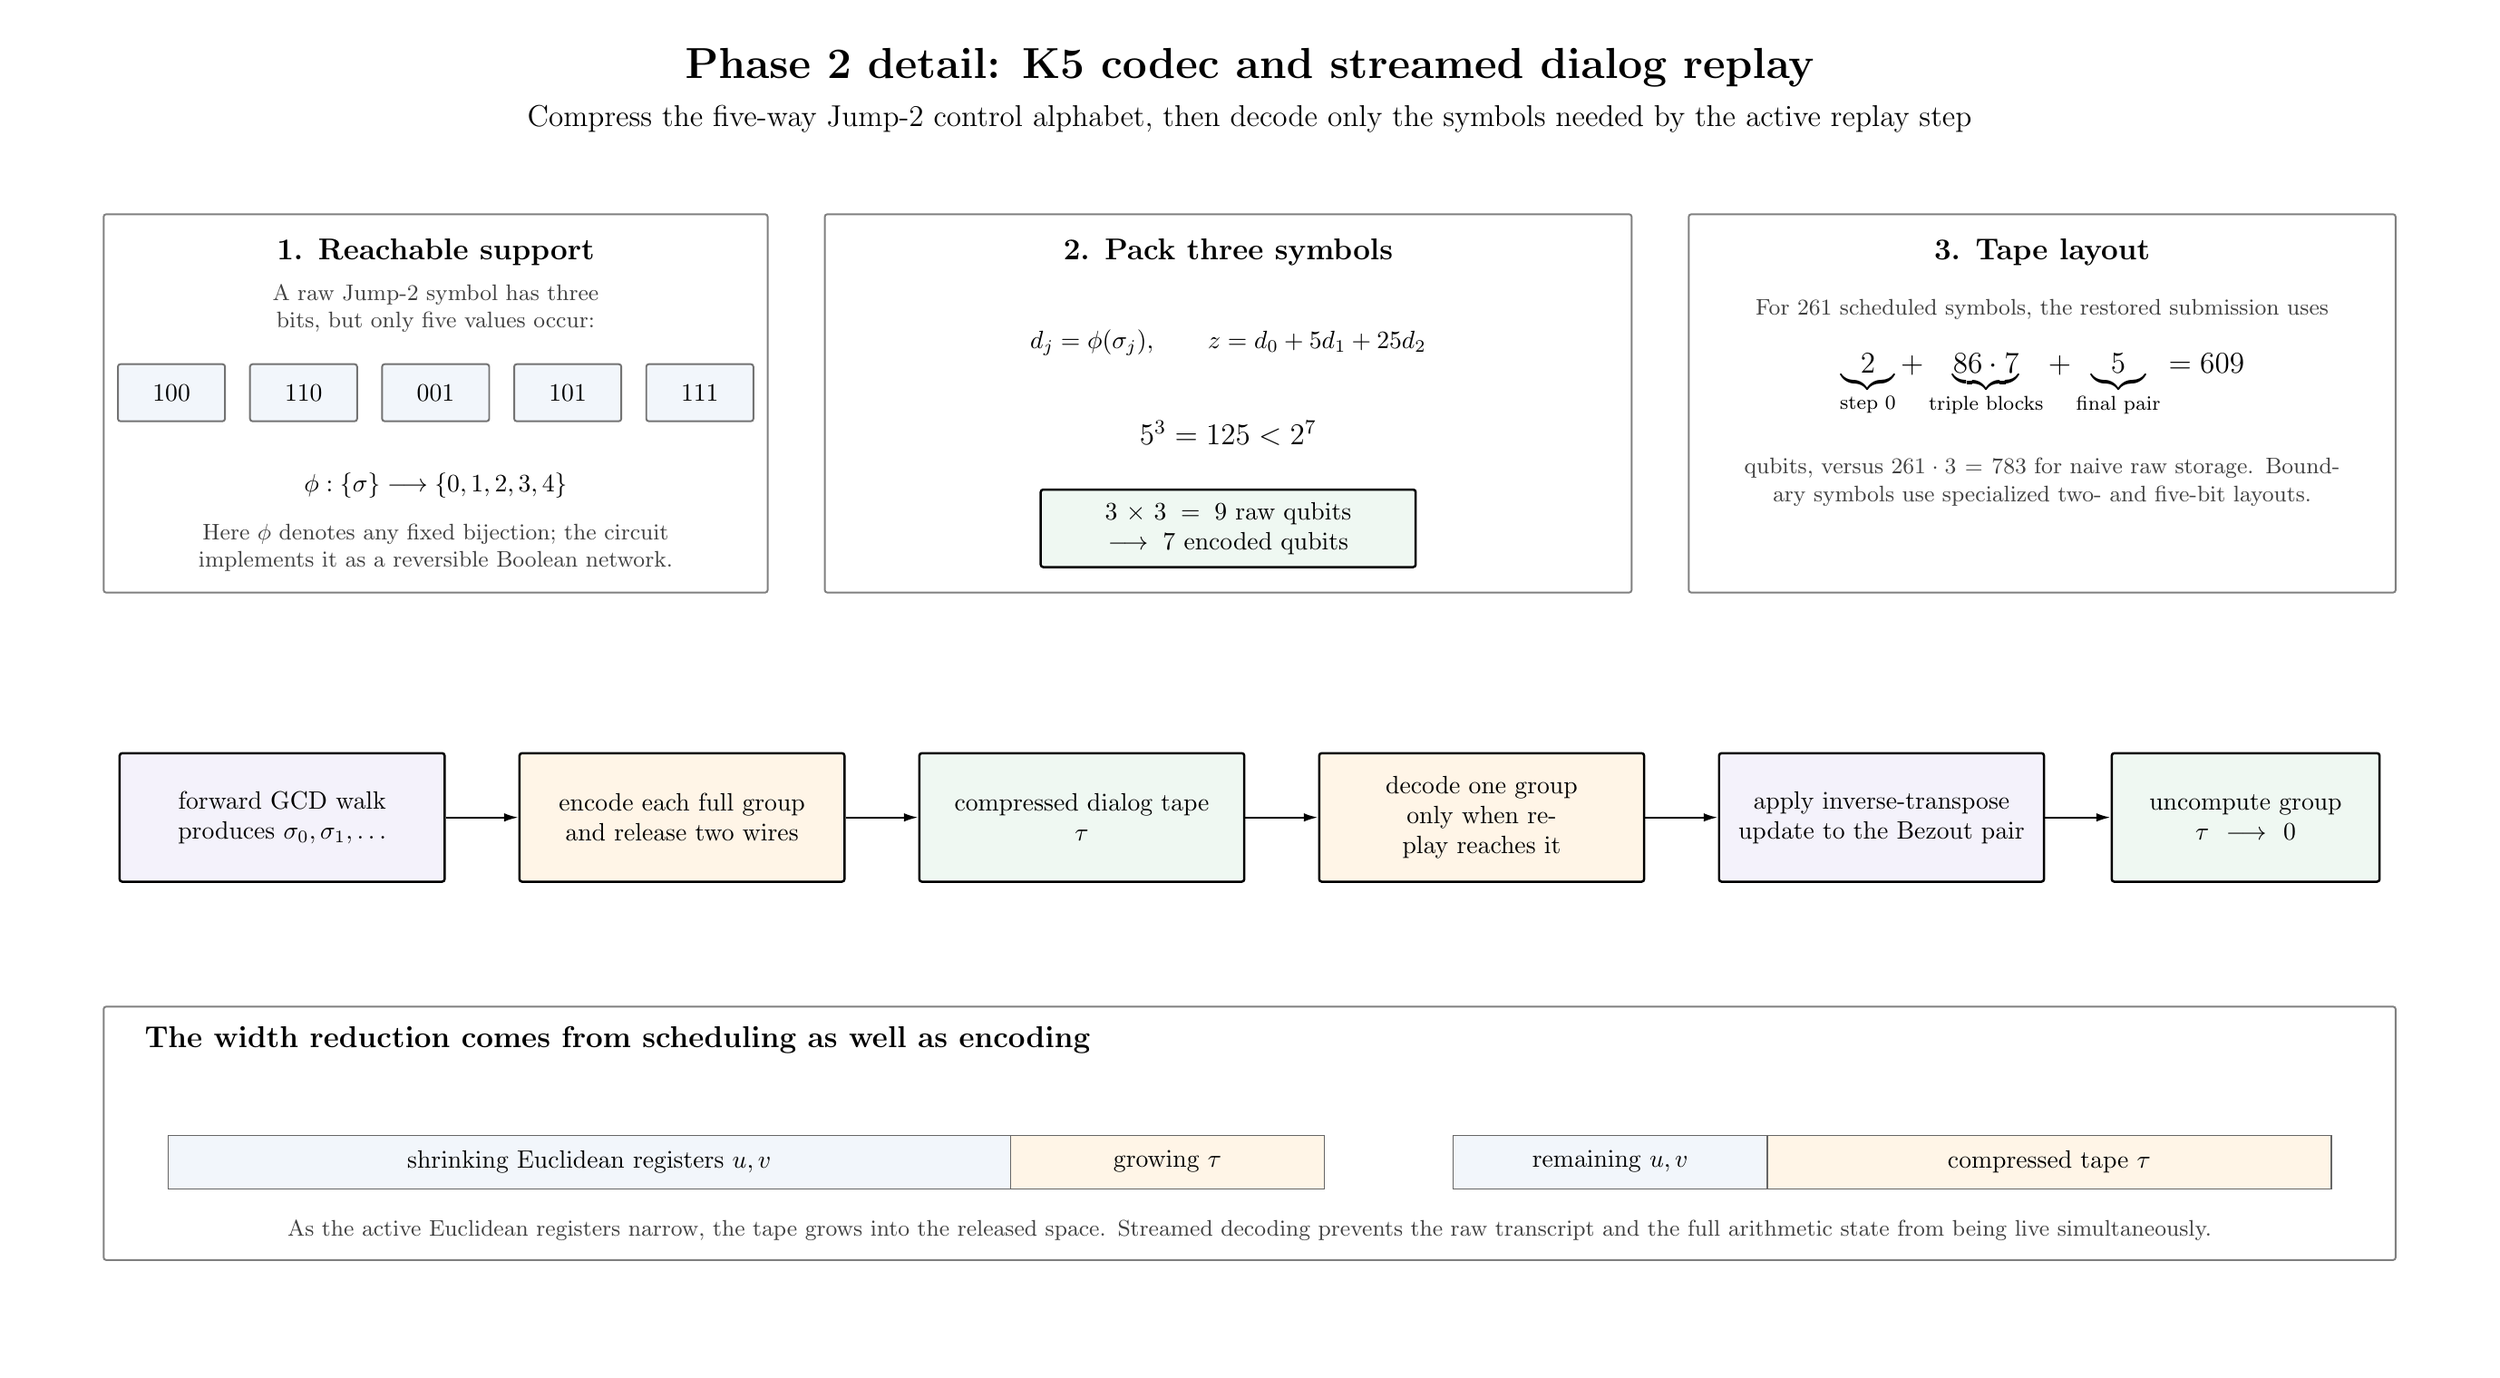
\begin{tikzpicture}[x=1cm,y=1cm]
  \path[use as bounding box] (0,0) rectangle (34.3,18.6);

  \node[font=\LARGE\bfseries] at (17.15,18.0)
    {Phase 2 detail: K5 codec and streamed dialog replay};
  \node[font=\large] at (17.15,17.28)
    {Compress the five-way Jump-2 control alphabet, then decode only the symbols needed by the active replay step};

  \draw[black!50, line width=0.7pt, rounded corners=1pt]
    (1.1,10.65) rectangle (10.4,15.95);
  \node[font=\large\bfseries] at (5.75,15.42) {1. Reachable support};
  \node[note, text width=8.2cm, align=center] at (5.75,14.63)
    {A raw Jump-2 symbol has three bits, but only five values occur:};
  \foreach \x/\sym in {2.05/{100},3.90/{110},5.75/{001},7.60/{101},9.45/{111}}
    {\node[registerbox, fill=gateblue, minimum width=15mm, minimum height=8mm]
       at (\x,13.45) {$\sym$};}
  \node[font=\normalsize] at (5.75,12.15)
    {$\phi:\{\sigma\}\longrightarrow\{0,1,2,3,4\}$};
  \node[note, text width=8.0cm, align=center] at (5.75,11.28)
    {Here $\phi$ denotes any fixed bijection; the circuit implements it as a reversible Boolean network.};

  \draw[black!50, line width=0.7pt, rounded corners=1pt]
    (11.2,10.65) rectangle (22.5,15.95);
  \node[font=\large\bfseries] at (16.85,15.42) {2. Pack three symbols};
  \node[font=\normalsize] at (16.85,14.15)
    {$d_j=\phi(\sigma_j),\qquad z=d_0+5d_1+25d_2$};
  \node[font=\large] at (16.85,12.88)
    {$5^3=125<2^7$};
  \node[detailgreen, text width=49mm, minimum height=10mm] at (16.85,11.55)
    {$3\times3=9$ raw qubits $\longrightarrow 7$ encoded qubits};

  \draw[black!50, line width=0.7pt, rounded corners=1pt]
    (23.3,10.65) rectangle (33.2,15.95);
  \node[font=\large\bfseries] at (28.25,15.42) {3. Tape layout};
  \node[note, text width=8.8cm, align=center] at (28.25,14.62)
    {For 261 scheduled symbols, the restored submission uses};
  \node[font=\large] at (28.25,13.55)
    {$\underbrace{2}_{\text{step 0}}+
      \underbrace{86\cdot7}_{\text{triple blocks}}+
      \underbrace{5}_{\text{final pair}}=609$};
  \node[note, text width=8.8cm, align=center] at (28.25,12.20)
    {qubits, versus $261\cdot3=783$ for naive raw storage.  Boundary symbols use specialized two- and five-bit layouts.};

  \node[detailviolet, text width=42mm, minimum height=18mm] (FWD) at (3.6,7.5)
    {forward GCD walk\\produces $\sigma_0,\sigma_1,\ldots$};
  \node[detailorange, text width=42mm, minimum height=18mm] (ENC) at (9.2,7.5)
    {encode each full group\\and release two wires};
  \node[detailgreen, text width=42mm, minimum height=18mm] (TAU) at (14.8,7.5)
    {compressed dialog tape\\$\tau$};
  \node[detailorange, text width=42mm, minimum height=18mm] (DEC) at (20.4,7.5)
    {decode one group\\only when replay reaches it};
  \node[detailviolet, text width=42mm, minimum height=18mm] (REP) at (26.0,7.5)
    {apply inverse-transpose\\update to the Bezout pair};
  \node[detailgreen, text width=34mm, minimum height=18mm] (CLR) at (31.1,7.5)
    {uncompute group\\$\tau\longrightarrow0$};
  \draw[flow] (FWD.east) -- (ENC.west);
  \draw[flow] (ENC.east) -- (TAU.west);
  \draw[flow] (TAU.east) -- (DEC.west);
  \draw[flow] (DEC.east) -- (REP.west);
  \draw[flow] (REP.east) -- (CLR.west);

  \draw[black!50, line width=0.7pt, rounded corners=1pt]
    (1.1,1.3) rectangle (33.2,4.85);
  \node[font=\large\bfseries, anchor=west] at (1.55,4.38)
    {The width reduction comes from scheduling as well as encoding};
  \draw[fill=gateblue, draw=black!60] (2.0,2.30) rectangle (13.8,3.05);
  \draw[fill=lookorange, draw=black!60] (13.8,2.30) rectangle (18.2,3.05);
  \node[font=\normalsize] at (7.9,2.68) {shrinking Euclidean registers $u,v$};
  \node[font=\normalsize] at (16.0,2.68) {growing $\tau$};
  \draw[fill=gateblue, draw=black!60] (20.0,2.30) rectangle (24.4,3.05);
  \draw[fill=lookorange, draw=black!60] (24.4,2.30) rectangle (32.3,3.05);
  \node[font=\normalsize] at (22.2,2.68) {remaining $u,v$};
  \node[font=\normalsize] at (28.35,2.68) {compressed tape $\tau$};
  \node[note, text width=29cm, align=center] at (17.15,1.72)
    {As the active Euclidean registers narrow, the tape grows into the released space.  Streamed decoding prevents the raw transcript and the full arithmetic state from being live simultaneously.};
\end{tikzpicture}

\newpage

% ============================================================================
% Page 9: width scheduling and temporary reuse used inside phase 2
% ============================================================================
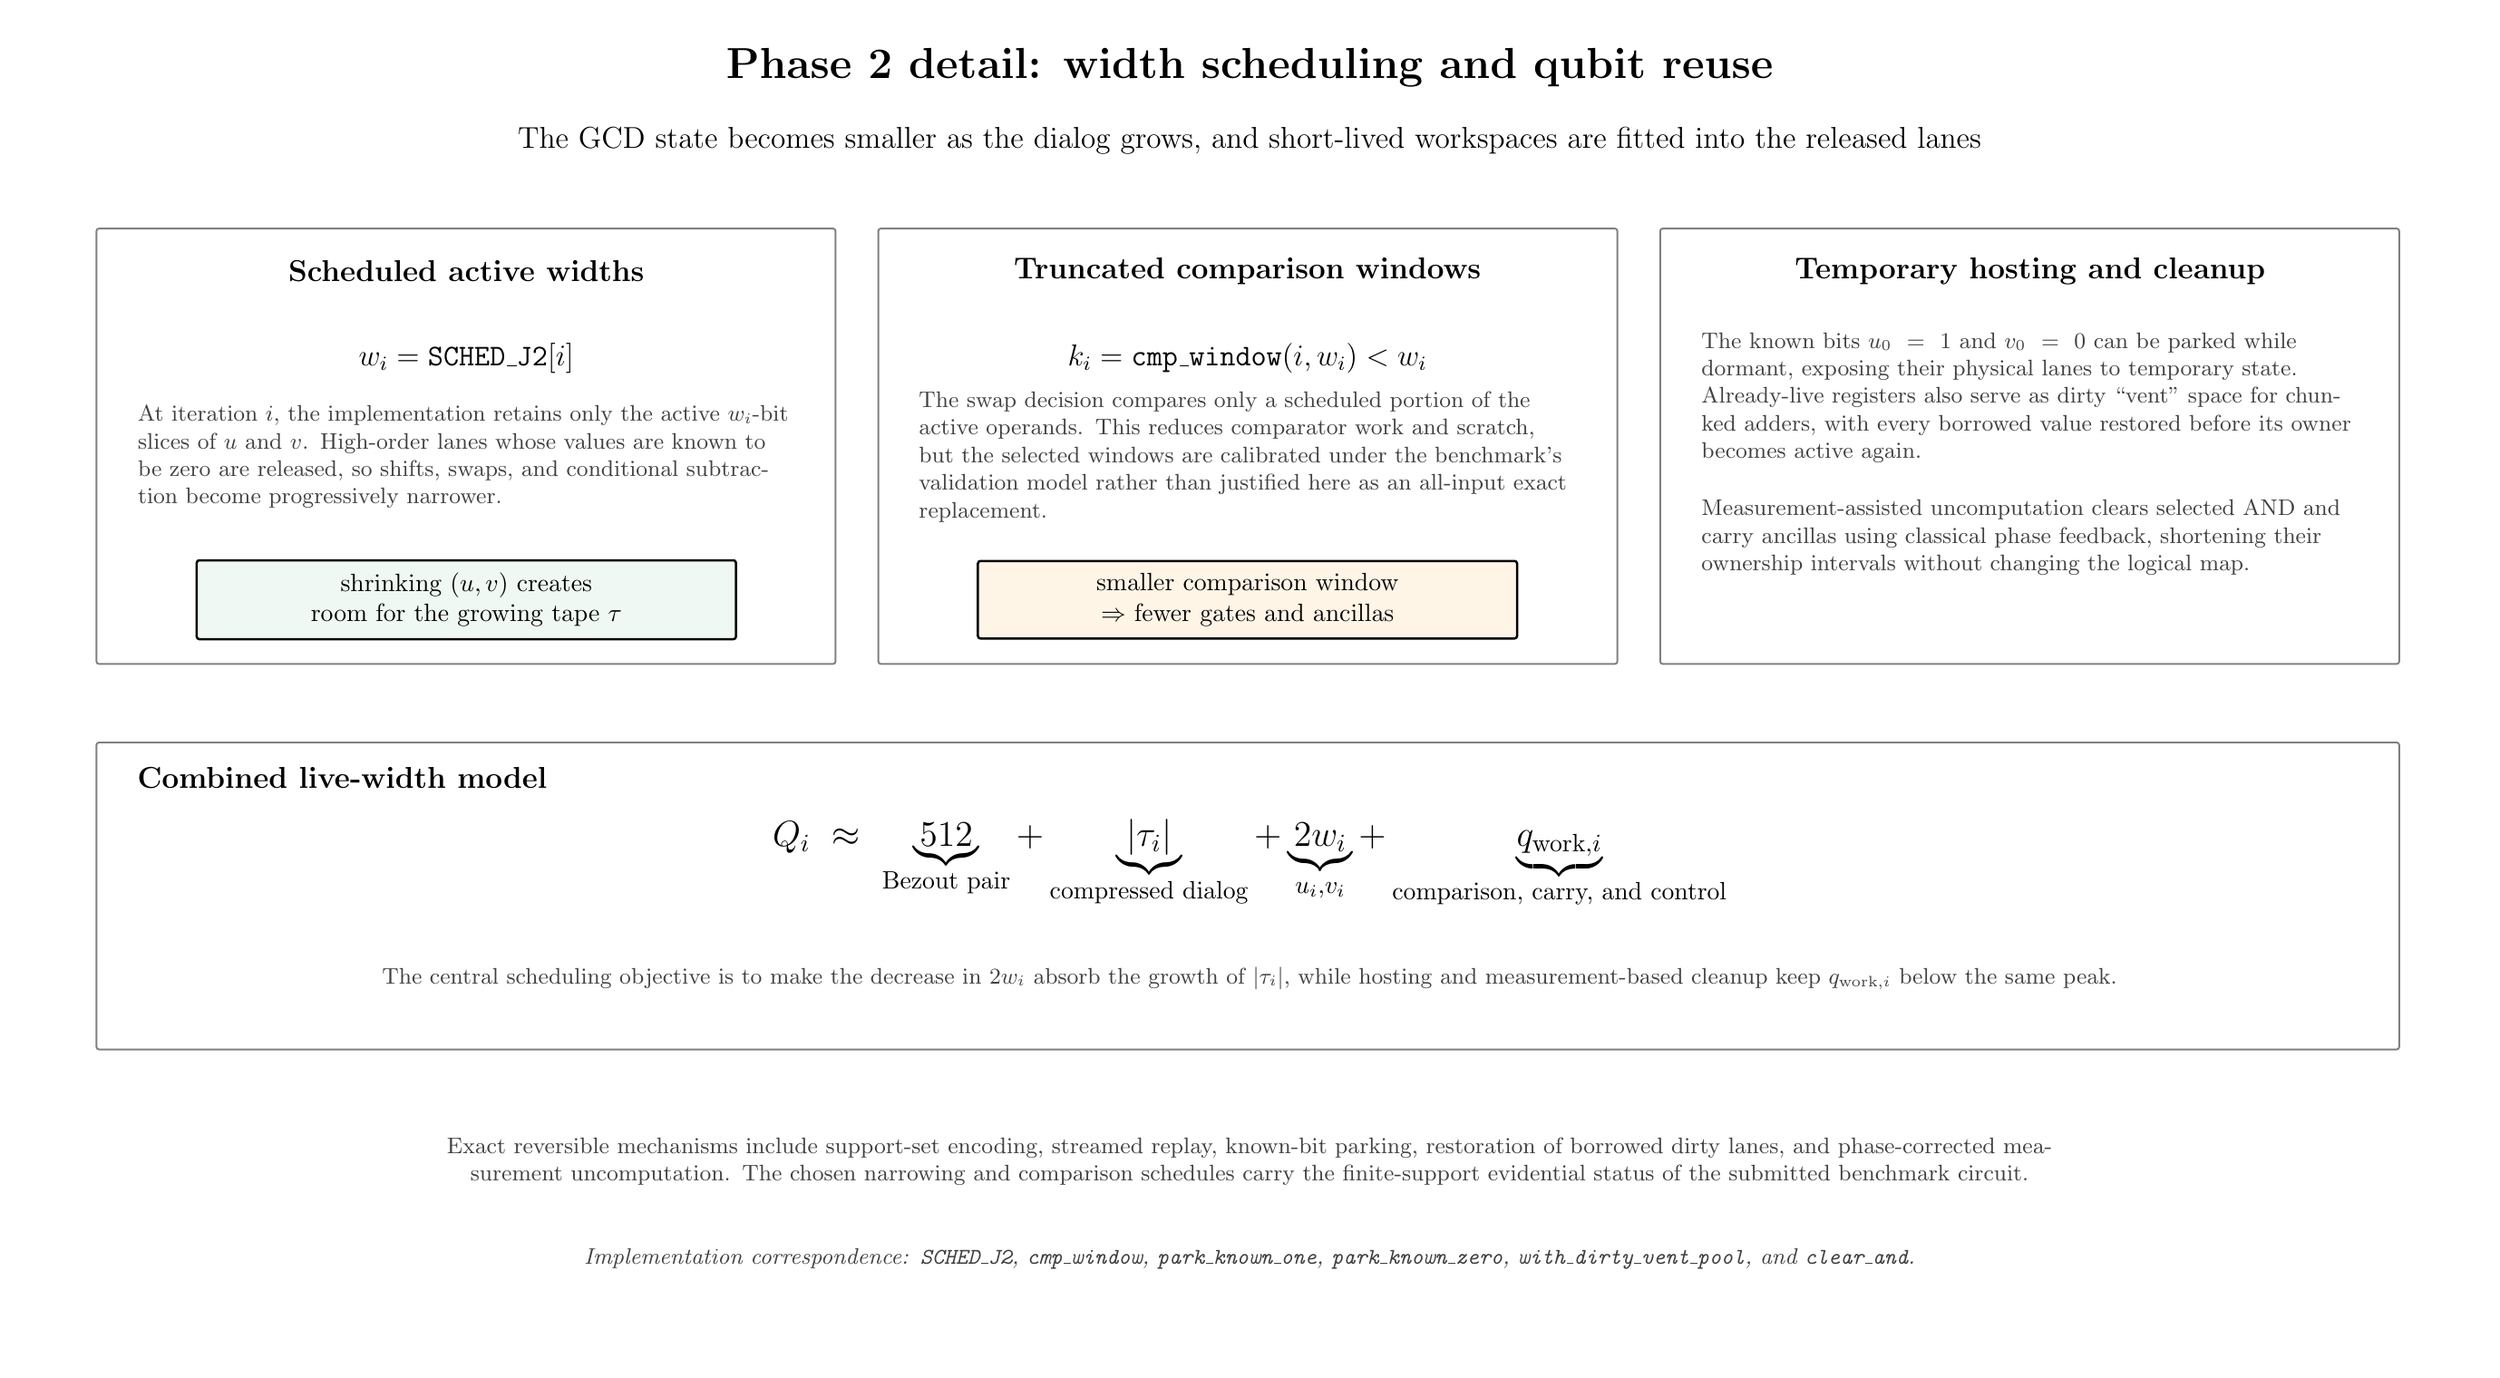
\begin{tikzpicture}[x=1cm,y=1cm]
  \path[use as bounding box] (0,0) rectangle (34.3,18.6);

  \node[font=\LARGE\bfseries] at (17.15,18.0)
    {Phase 2 detail: width scheduling and qubit reuse};
  \node[font=\large] at (17.15,16.98)
    {The GCD state becomes smaller as the dialog grows, and short-lived workspaces are fitted into the released lanes};

  \draw[black!50, line width=0.7pt, rounded corners=1pt]
    (1.0,9.65) rectangle (11.35,15.75);
  \node[font=\large\bfseries] at (6.18,15.15)
    {Scheduled active widths};
  \node[font=\large] at (6.18,13.93)
    {$w_i=\texttt{SCHED\_J2}[i]$};
  \node[note, text width=9.2cm, align=left] at (6.18,12.55)
    {At iteration $i$, the implementation retains only the active $w_i$-bit slices of $u$ and $v$.  High-order lanes whose values are known to be zero are released, so shifts, swaps, and conditional subtraction become progressively narrower.};
  \node[detailgreen, text width=72mm, minimum height=10mm] at (6.18,10.55)
    {shrinking $(u,v)$ creates room for the growing tape $\tau$};

  \draw[black!50, line width=0.7pt, rounded corners=1pt]
    (11.95,9.65) rectangle (22.3,15.75);
  \node[font=\large\bfseries] at (17.12,15.15)
    {Truncated comparison windows};
  \node[font=\large] at (17.12,13.93)
    {$k_i=\texttt{cmp\_window}(i,w_i)<w_i$};
  \node[note, text width=9.2cm, align=left] at (17.12,12.55)
    {The swap decision compares only a scheduled portion of the active operands.  This reduces comparator work and scratch, but the selected windows are calibrated under the benchmark's validation model rather than justified here as an all-input exact replacement.};
  \node[detailorange, text width=72mm, minimum height=10mm] at (17.12,10.55)
    {smaller comparison window $\Rightarrow$ fewer gates and ancillas};

  \draw[black!50, line width=0.7pt, rounded corners=1pt]
    (22.9,9.65) rectangle (33.25,15.75);
  \node[font=\large\bfseries] at (28.08,15.15)
    {Temporary hosting and cleanup};
  \node[note, text width=9.2cm, align=left] at (28.08,13.38)
    {The known bits $u_0=1$ and $v_0=0$ can be parked while dormant, exposing their physical lanes to temporary state.  Already-live registers also serve as dirty ``vent'' space for chunked adders, with every borrowed value restored before its owner becomes active again.};
  \node[note, text width=9.2cm, align=left] at (28.08,11.42)
    {Measurement-assisted uncomputation clears selected AND and carry ancillas using classical phase feedback, shortening their ownership intervals without changing the logical map.};

  \draw[black!50, line width=0.7pt, rounded corners=1pt]
    (1.0,4.25) rectangle (33.25,8.55);
  \node[font=\large\bfseries, anchor=west] at (1.45,8.05)
    {Combined live-width model};
  \node[font=\Large] at (17.15,6.85)
    {$Q_i\ \approx\ \underbrace{512}_{\text{Bezout pair}}
      +\underbrace{|\tau_i|}_{\text{compressed dialog}}
      +\underbrace{2w_i}_{u_i,v_i}
      +\underbrace{q_{\mathrm{work},i}}_{\text{comparison, carry, and control}}$};
  \node[note, text width=29.5cm, align=center] at (17.15,5.25)
    {The central scheduling objective is to make the decrease in $2w_i$ absorb the growth of $|\tau_i|$, while hosting and measurement-based cleanup keep $q_{\mathrm{work},i}$ below the same peak.};

  \node[note, text width=30cm, align=center] at (17.15,2.68)
    {Exact reversible mechanisms include support-set encoding, streamed replay, known-bit parking, restoration of borrowed dirty lanes, and phase-corrected measurement uncomputation.  The chosen narrowing and comparison schedules carry the finite-support evidential status of the submitted benchmark circuit.};
  \node[note, text width=30cm, align=center, font=\small\itshape] at (17.15,1.32)
    {Implementation correspondence: \texttt{SCHED\_J2}, \texttt{cmp\_window}, \texttt{park\_known\_one}, \texttt{park\_known\_zero}, \texttt{with\_dirty\_vent\_pool}, and \texttt{clear\_and}.};
\end{tikzpicture}

\newpage

% ============================================================================
% Page 10: phase 3, prepare X workspace
% ============================================================================
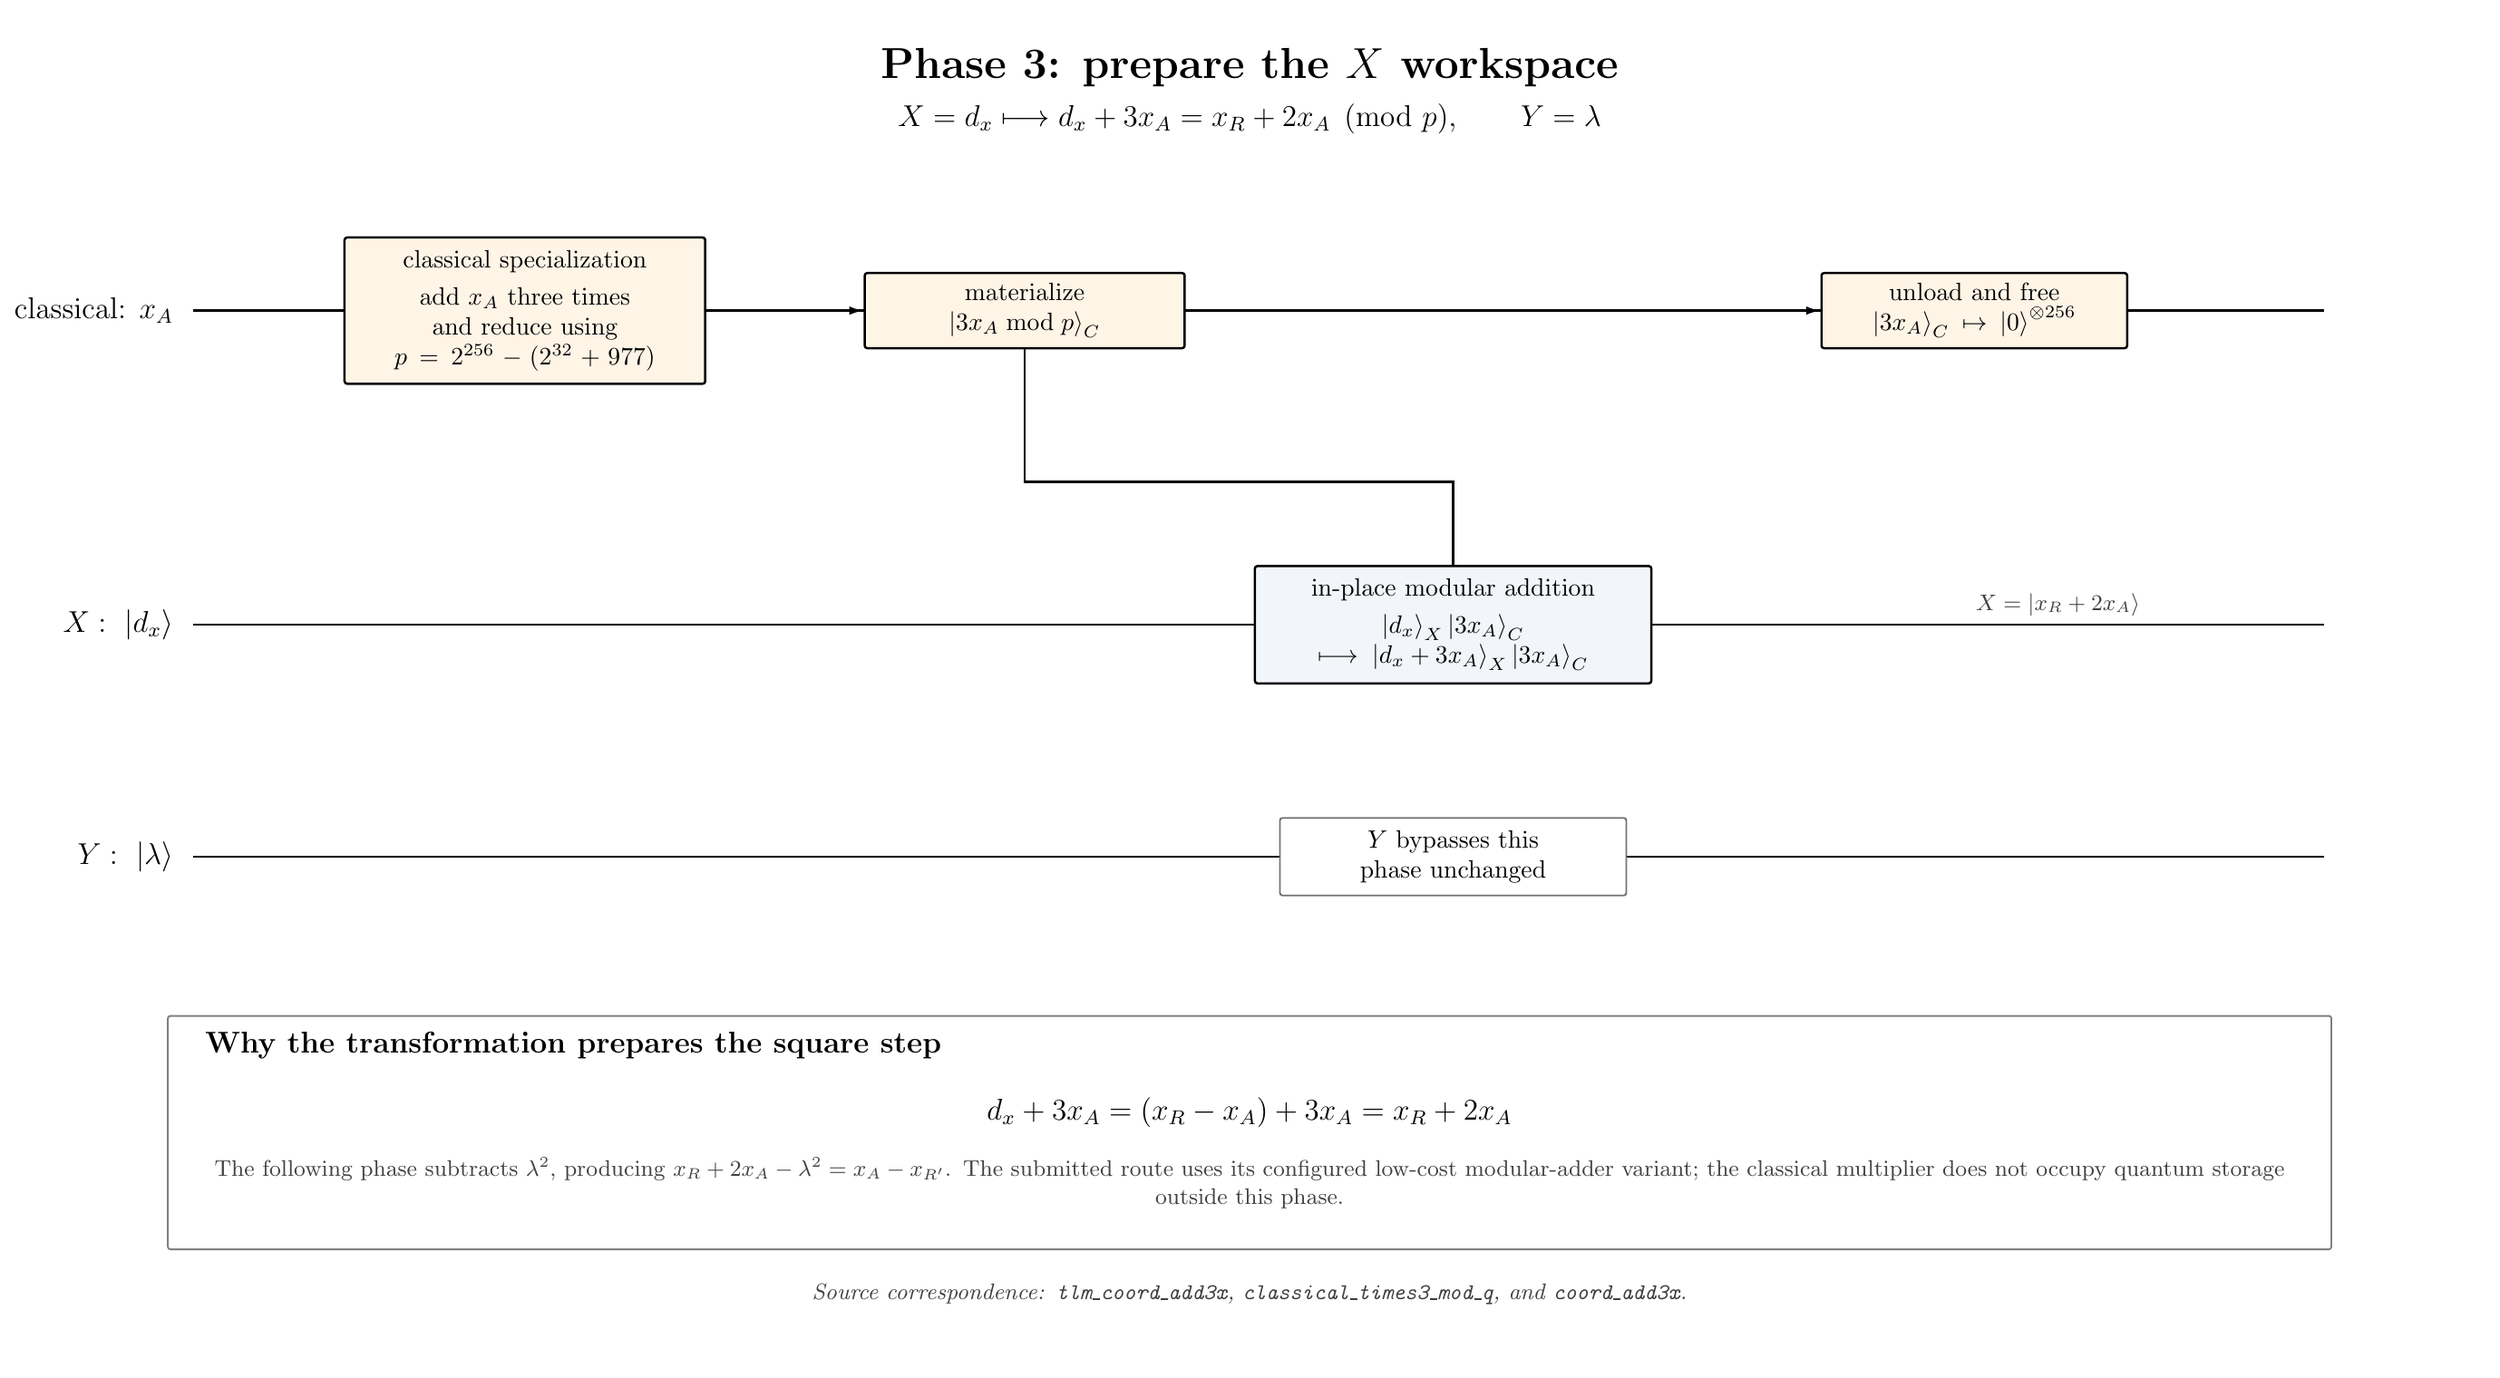
\begin{tikzpicture}[x=1cm,y=1cm]
  \path[use as bounding box] (0,0) rectangle (34.3,18.6);

  \node[font=\LARGE\bfseries] at (17.15,18.0)
    {Phase 3: prepare the $X$ workspace};
  \node[font=\large] at (17.15,17.28)
    {$X=d_x\longmapsto d_x+3x_A=x_R+2x_A\pmod p,\qquad Y=\lambda$};

  \node[lab, anchor=east] at (2.2,14.6) {classical: $x_A$};
  \draw[wire] (2.35,14.6) -- (32.2,14.6);
  \node[detailorange, text width=47mm] (C3) at (7.0,14.6)
    {classical specialization\\[1mm]
     add $x_A$ three times and reduce using\\
     $p=2^{256}-(2^{32}+977)$};
  \node[lookup, text width=42mm] (LOAD3) at (14.0,14.6)
    {materialize\\$\ket{3x_A\bmod p}_C$};
  \draw[flow] (C3.east) -- (LOAD3.west);

  \node[lab, anchor=east] at (2.2,10.2) {$X:\ \ket{d_x}$};
  \draw[wire] (2.35,10.2) -- (32.2,10.2);
  \node[detail, text width=52mm] (ADD3) at (20.0,10.2)
    {in-place modular addition\\[1mm]
     $\ket{d_x}_X\ket{3x_A}_C$\\
     $\longmapsto\ket{d_x+3x_A}_X\ket{3x_A}_C$};
  \draw[wire] (LOAD3.south) -- (14.0,12.2) -- (20.0,12.2) -- (ADD3.north);
  \node[lookup, text width=40mm] (UNLOAD3) at (27.3,14.6)
    {unload and free\\$\ket{3x_A}_C\mapsto\ket{0}^{\otimes256}$};
  \draw[flow] (LOAD3.east) -- (UNLOAD3.west);
  \node[note, anchor=south west] at (27.2,10.2) {$X=\ket{x_R+2x_A}$};

  \node[lab, anchor=east] at (2.2,6.95) {$Y:\ \ket{\lambda}$};
  \draw[wire] (2.35,6.95) -- (32.2,6.95);
  \node[registerbox, text width=45mm] at (20.0,6.95)
    {$Y$ bypasses this phase unchanged};

  \draw[black!50, line width=0.7pt, rounded corners=1pt]
    (2.0,1.45) rectangle (32.3,4.72);
  \node[font=\large\bfseries, anchor=west] at (2.4,4.30)
    {Why the transformation prepares the square step};
  \node[font=\large] at (17.15,3.36)
    {$d_x+3x_A=(x_R-x_A)+3x_A=x_R+2x_A$};
  \node[note, text width=29cm, align=center] at (17.15,2.38)
    {The following phase subtracts $\lambda^2$, producing $x_R+2x_A-\lambda^2=x_A-x_{R'}$.  The submitted route uses its configured low-cost modular-adder variant; the classical multiplier does not occupy quantum storage outside this phase.};
  \node[note, text width=29cm, align=center, font=\small\itshape] at (17.15,0.82)
    {Source correspondence: \texttt{tlm\_coord\_add3x}, \texttt{classical\_times3\_mod\_q}, and \texttt{coord\_add3x}.};
\end{tikzpicture}

\newpage

% ============================================================================
% Page 11: phase 4, specialized square
% ============================================================================
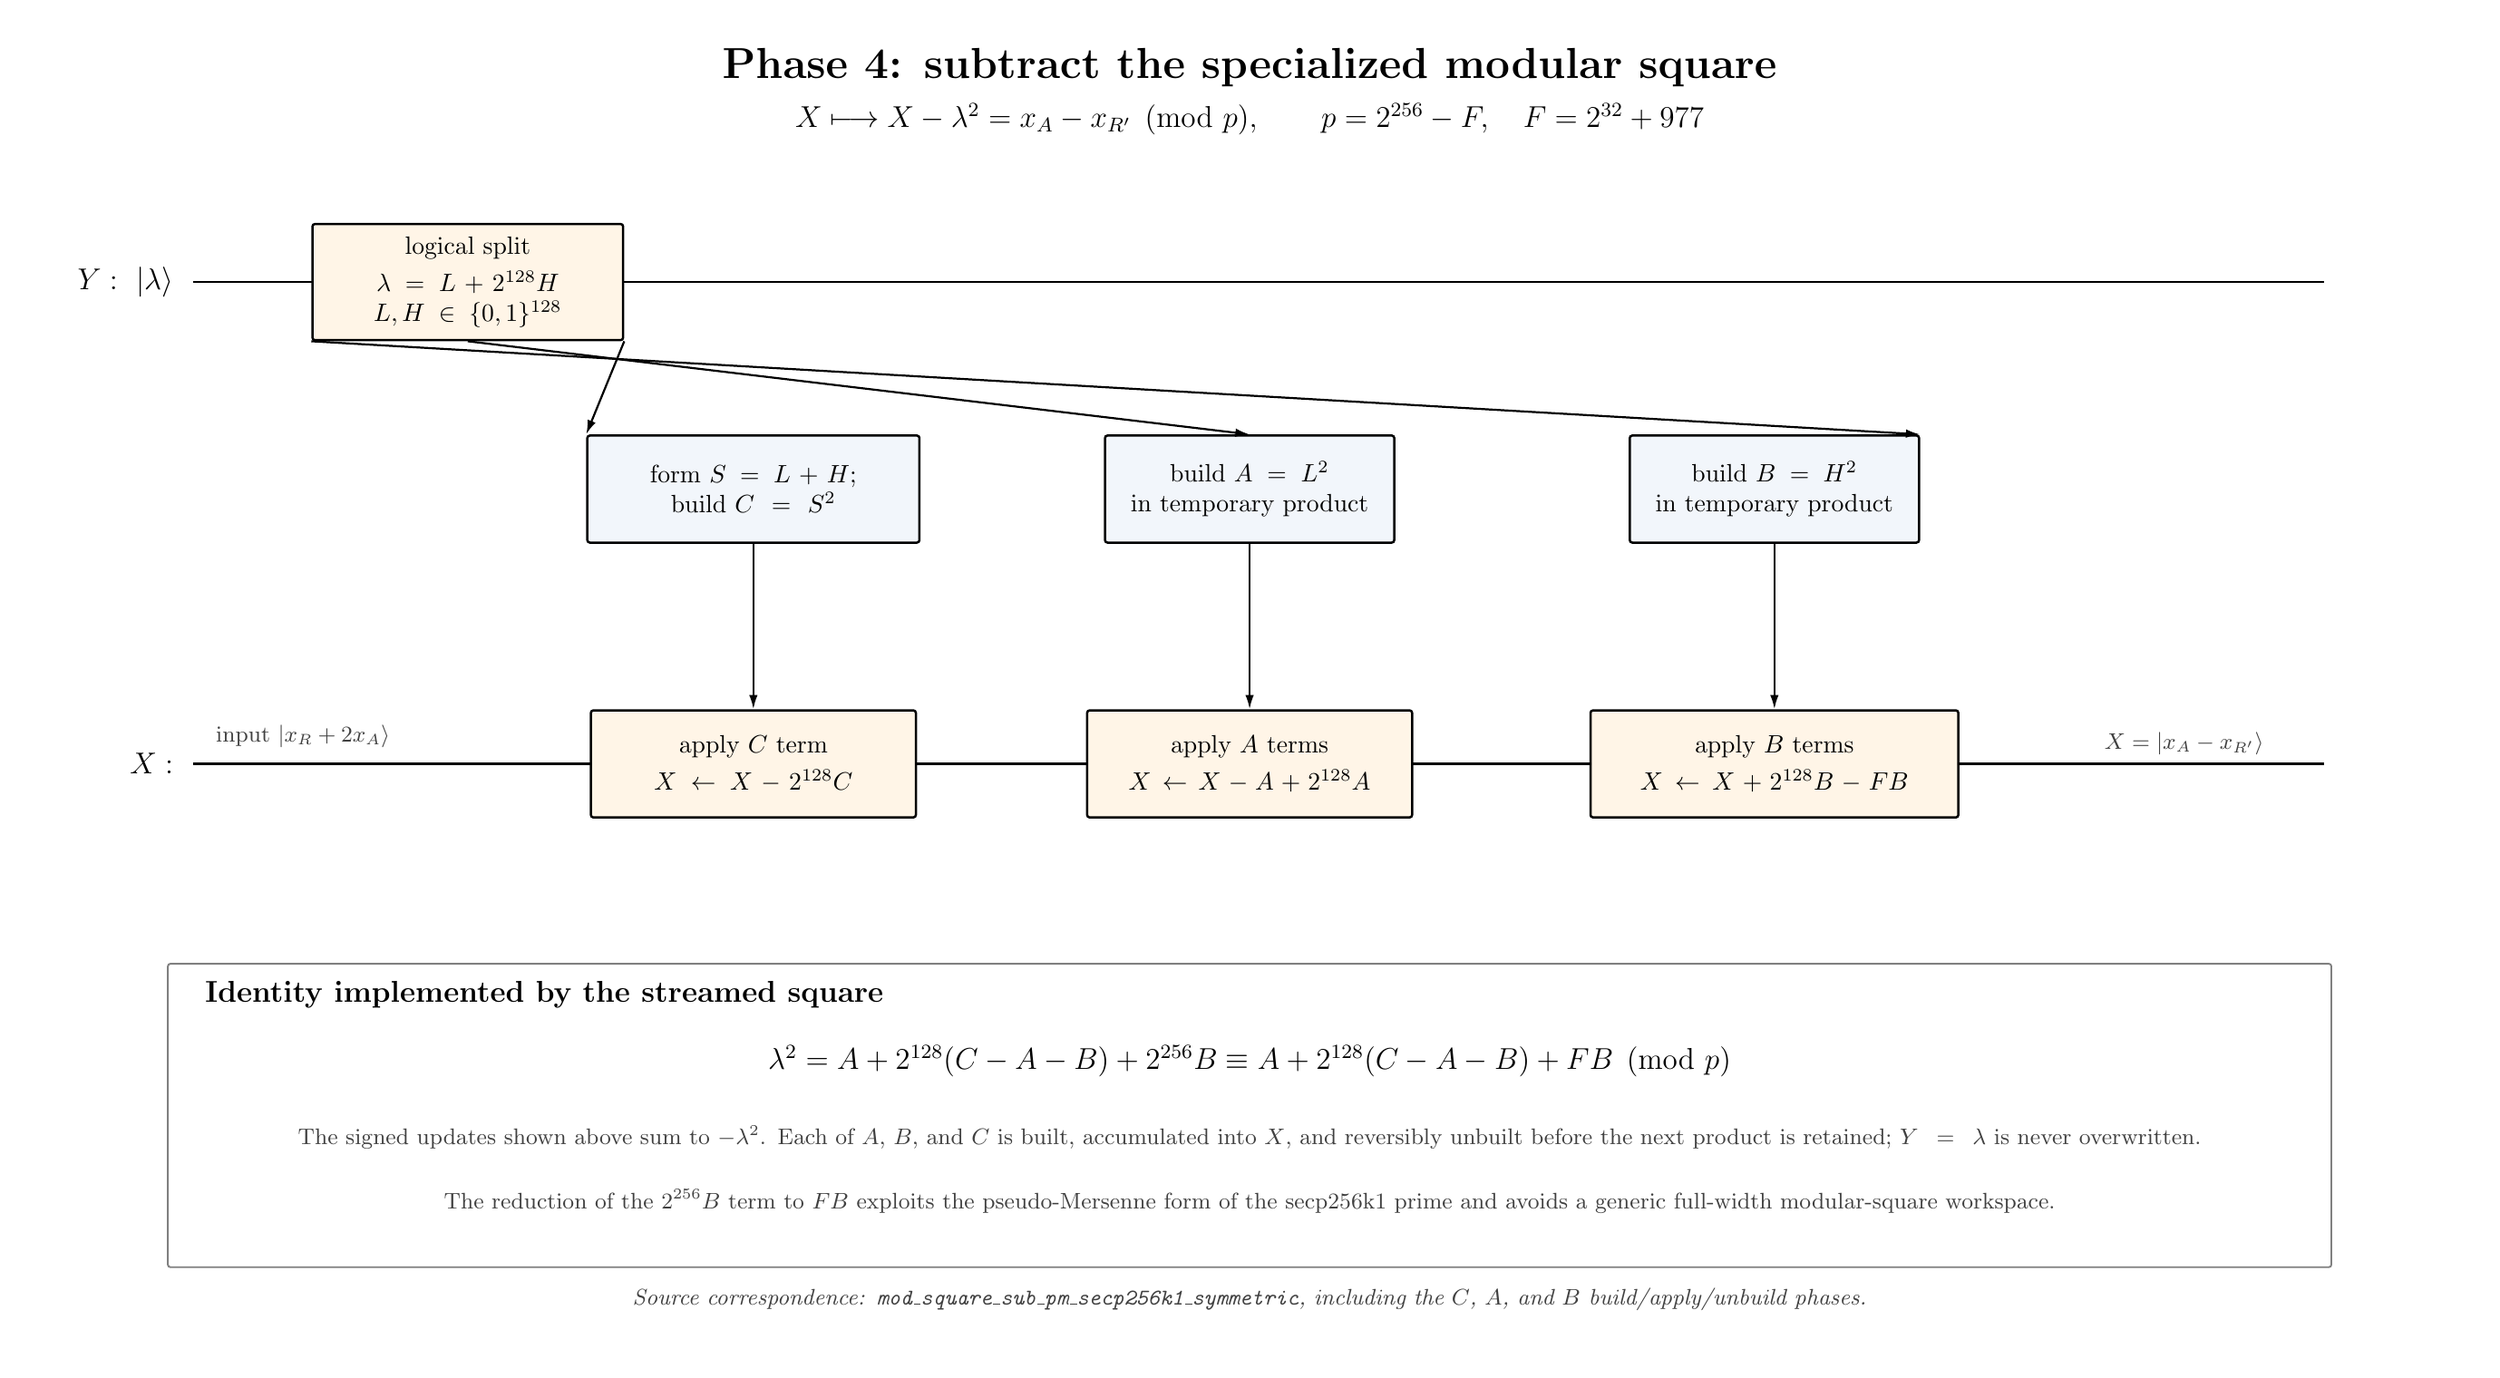
\begin{tikzpicture}[x=1cm,y=1cm]
  \path[use as bounding box] (0,0) rectangle (34.3,18.6);

  \node[font=\LARGE\bfseries] at (17.15,18.0)
    {Phase 4: subtract the specialized modular square};
  \node[font=\large] at (17.15,17.28)
    {$X\longmapsto X-\lambda^2=x_A-x_{R'}\pmod p,\qquad p=2^{256}-F,\quad F=2^{32}+977$};

  \node[lab, anchor=east] at (2.2,15.0) {$Y:\ \ket{\lambda}$};
  \draw[wire] (2.35,15.0) -- (32.2,15.0);
  \node[detailorange, text width=40mm] (SPLIT) at (6.2,15.0)
    {logical split\\[1mm]
     $\lambda=L+2^{128}H$\\
     $L,H\in\{0,1\}^{128}$};

  \node[detail, text width=43mm] (PC) at (10.2,12.1)
    {form $S=L+H$;\\build $C=S^2$};
  \node[detail, text width=37mm] (PA) at (17.15,12.1)
    {build $A=L^2$\\in temporary product};
  \node[detail, text width=37mm] (PB) at (24.5,12.1)
    {build $B=H^2$\\in temporary product};
  \draw[flow] (SPLIT.south east) -- (PC.north west);
  \draw[flow] (SPLIT.south) -- (PA.north);
  \draw[flow] (SPLIT.south west) -- (PB.north east);

  \node[lab, anchor=east] at (2.2,8.25) {$X:$};
  \node[note, anchor=west] at (2.55,8.63)
    {input $\ket{x_R+2x_A}$};
  \draw[wire] (2.35,8.25) -- (32.2,8.25);
  \node[detailorange, text width=42mm] (AC) at (10.2,8.25)
    {apply $C$ term\\[1mm]
     $X\gets X-2^{128}C$};
  \node[detailorange, text width=42mm] (AA) at (17.15,8.25)
    {apply $A$ terms\\[1mm]
     $X\gets X-A+2^{128}A$};
  \node[detailorange, text width=48mm] (AB) at (24.5,8.25)
    {apply $B$ terms\\[1mm]
     $X\gets X+2^{128}B-FB$};
  \draw[flow] (PC.south) -- (AC.north);
  \draw[flow] (PA.south) -- (AA.north);
  \draw[flow] (PB.south) -- (AB.north);
  \node[note, anchor=south west] at (29.0,8.25) {$X=\ket{x_A-x_{R'}}$};

  \draw[black!50, line width=0.7pt, rounded corners=1pt]
    (2.0,1.2) rectangle (32.3,5.45);
  \node[font=\large\bfseries, anchor=west] at (2.4,5.02)
    {Identity implemented by the streamed square};
  \node[font=\large] at (17.15,4.08)
    {$\lambda^2=A+2^{128}(C-A-B)+2^{256}B
      \equiv A+2^{128}(C-A-B)+FB\pmod p$};
  \node[note, text width=29cm, align=center] at (17.15,3.02)
    {The signed updates shown above sum to $-\lambda^2$.  Each of $A$, $B$, and $C$ is built, accumulated into $X$, and reversibly unbuilt before the next product is retained; $Y=\lambda$ is never overwritten.};
  \node[note, text width=29cm, align=center] at (17.15,2.12)
    {The reduction of the $2^{256}B$ term to $FB$ exploits the pseudo-Mersenne form of the secp256k1 prime and avoids a generic full-width modular-square workspace.};
  \node[note, text width=29cm, align=center, font=\small\itshape] at (17.15,0.75)
    {Source correspondence: \texttt{mod\_square\_sub\_pm\_secp256k1\_symmetric}, including the $C$, $A$, and $B$ build/apply/unbuild phases.};
\end{tikzpicture}

\newpage

% ============================================================================
% Page 12: phase 4 detail, streamed pseudo-Mersenne square
% ============================================================================
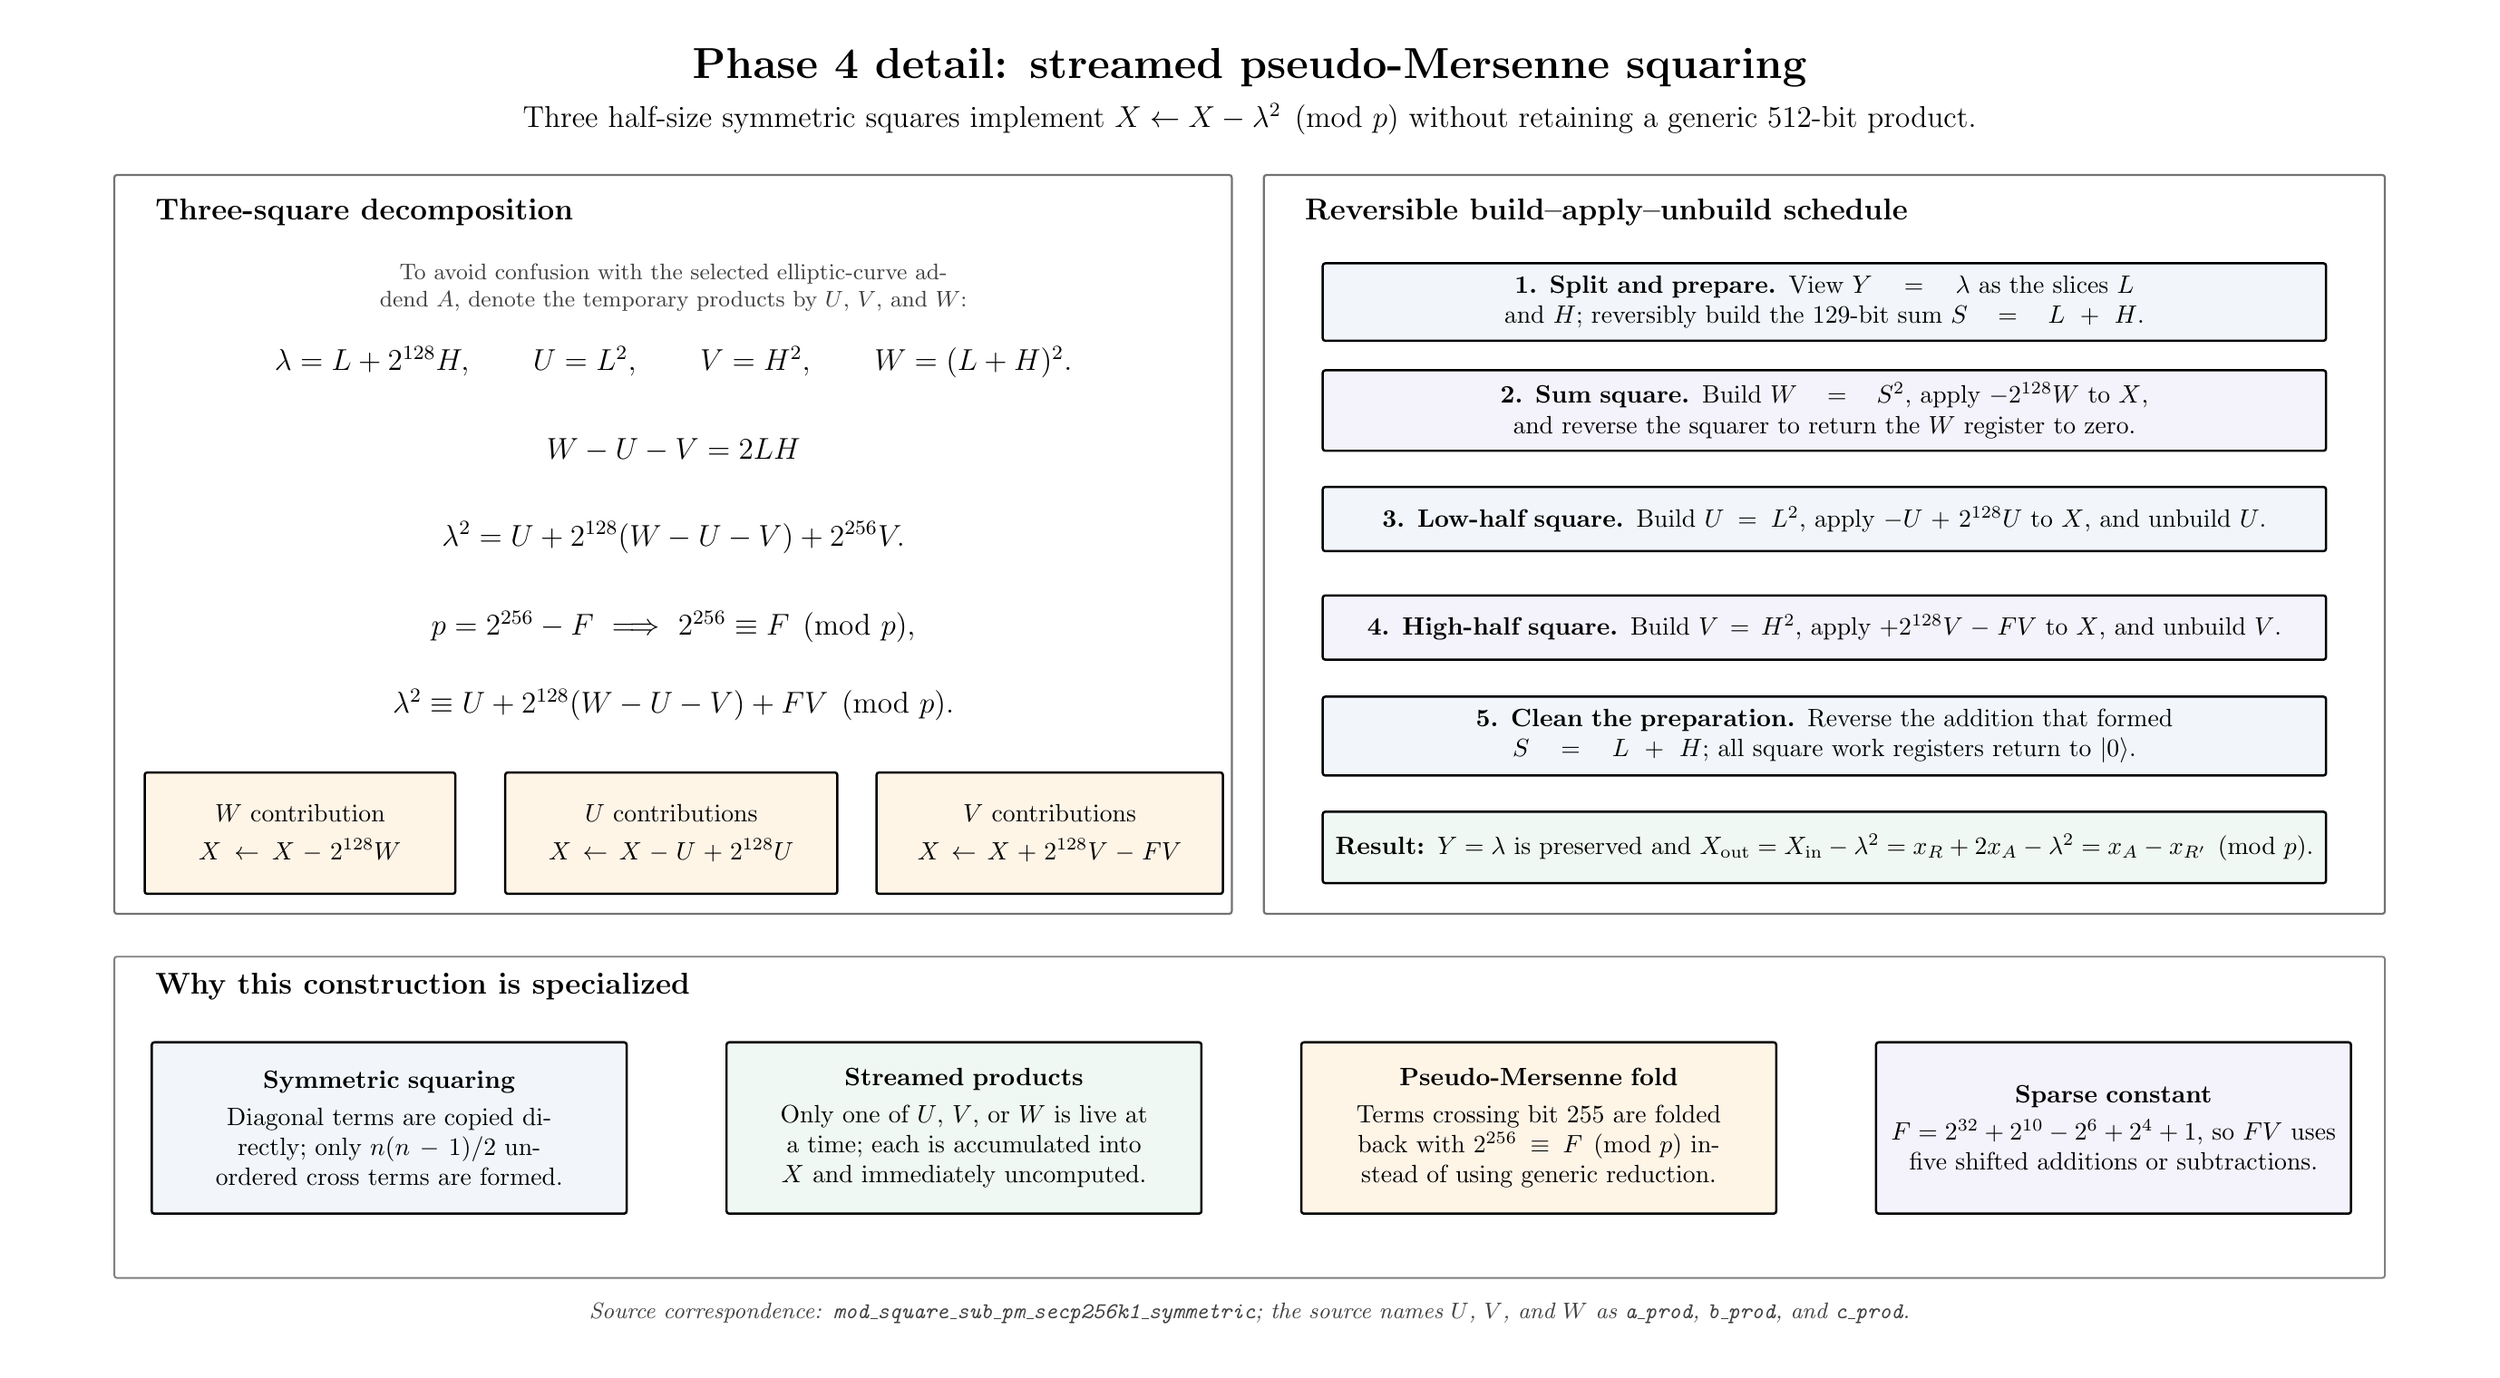
\begin{tikzpicture}[x=1cm,y=1cm]
  \path[use as bounding box] (0,0) rectangle (34.3,18.6);

  \node[font=\LARGE\bfseries] at (17.15,18.0)
    {Phase 4 detail: streamed pseudo-Mersenne squaring};
  \node[font=\large] at (17.15,17.28)
    {Three half-size symmetric squares implement $X\gets X-\lambda^2\pmod p$ without retaining a generic $512$-bit product.};

  % Algebra panel.
  \draw[black!55, line width=0.8pt, rounded corners=1pt]
    (1.25,6.15) rectangle (16.90,16.50);
  \node[font=\large\bfseries, anchor=west] at (1.70,15.98)
    {Three-square decomposition};
  \node[note, text width=14.4cm, align=center] at (9.08,14.92)
    {To avoid confusion with the selected elliptic-curve addend $A$, denote the temporary products by $U$, $V$, and $W$:};
  \node[font=\large] at (9.08,13.88)
    {$\lambda=L+2^{128}H,\qquad U=L^2,\qquad V=H^2,\qquad W=(L+H)^2.$};
  \node[font=\large] at (9.08,12.65)
    {$W-U-V=2LH$};
  \node[font=\large] at (9.08,11.42)
    {$\lambda^2=U+2^{128}(W-U-V)+2^{256}V.$};
  \node[font=\large] at (9.08,10.17)
    {$p=2^{256}-F\ \Longrightarrow\ 2^{256}\equiv F\pmod p,$};
  \node[font=\large] at (9.08,9.08)
    {$\lambda^2\equiv U+2^{128}(W-U-V)+FV\pmod p.$};

  \node[detailorange, text width=40mm, minimum height=17mm] at (3.85,7.28)
    {$W$ contribution\\[1mm]
     $X\gets X-2^{128}W$};
  \node[detailorange, text width=43mm, minimum height=17mm] at (9.05,7.28)
    {$U$ contributions\\[1mm]
     $X\gets X-U+2^{128}U$};
  \node[detailorange, text width=45mm, minimum height=17mm] at (14.35,7.28)
    {$V$ contributions\\[1mm]
     $X\gets X+2^{128}V-FV$};

  % Reversible schedule panel.
  \draw[black!55, line width=0.8pt, rounded corners=1pt]
    (17.35,6.15) rectangle (33.05,16.50);
  \node[font=\large\bfseries, anchor=west] at (17.80,15.98)
    {Reversible build--apply--unbuild schedule};

  \node[detail, text width=137mm, minimum height=9mm] at (25.20,14.72)
    {\textbf{1. Split and prepare.} View $Y=\lambda$ as the slices $L$ and $H$; reversibly build the $129$-bit sum $S=L+H$.};
  \node[detailviolet, text width=137mm, minimum height=9mm] at (25.20,13.20)
    {\textbf{2. Sum square.} Build $W=S^2$, apply $-2^{128}W$ to $X$, and reverse the squarer to return the $W$ register to zero.};
  \node[detail, text width=137mm, minimum height=9mm] at (25.20,11.68)
    {\textbf{3. Low-half square.} Build $U=L^2$, apply $-U+2^{128}U$ to $X$, and unbuild $U$.};
  \node[detailviolet, text width=137mm, minimum height=9mm] at (25.20,10.16)
    {\textbf{4. High-half square.} Build $V=H^2$, apply $+2^{128}V-FV$ to $X$, and unbuild $V$.};
  \node[detail, text width=137mm, minimum height=9mm] at (25.20,8.64)
    {\textbf{5. Clean the preparation.} Reverse the addition that formed $S=L+H$; all square work registers return to $\ket{0}$.};
  \node[detailgreen, text width=137mm, minimum height=10mm] at (25.20,7.08)
    {\textbf{Result:} $Y=\lambda$ is preserved and
     $X_{\mathrm{out}}=X_{\mathrm{in}}-\lambda^2=x_R+2x_A-\lambda^2=x_A-x_{R'}\pmod p$.};

  % Resource-saving mechanisms.
  \draw[black!50, line width=0.7pt, rounded corners=1pt]
    (1.25,1.05) rectangle (33.05,5.55);
  \node[font=\large\bfseries, anchor=west] at (1.70,5.13)
    {Why this construction is specialized};
  \node[detail, text width=63mm, minimum height=24mm] at (5.10,3.15)
    {\textbf{Symmetric squaring}\\[1mm]
     Diagonal terms are copied directly; only $n(n-1)/2$ unordered cross terms are formed.};
  \node[detailgreen, text width=63mm, minimum height=24mm] at (13.15,3.15)
    {\textbf{Streamed products}\\[1mm]
     Only one of $U$, $V$, or $W$ is live at a time; each is accumulated into $X$ and immediately uncomputed.};
  \node[detailorange, text width=63mm, minimum height=24mm] at (21.20,3.15)
    {\textbf{Pseudo-Mersenne fold}\\[1mm]
     Terms crossing bit $255$ are folded back with $2^{256}\equiv F\pmod p$ instead of using generic reduction.};
  \node[detailviolet, text width=63mm, minimum height=24mm] at (29.25,3.15)
    {\textbf{Sparse constant}\\[1mm]
     $F=2^{32}+2^{10}-2^6+2^4+1$, so $FV$ uses five shifted additions or subtractions.};

  \node[note, text width=31cm, align=center, font=\small\itshape] at (17.15,0.55)
    {Source correspondence: \texttt{mod\_square\_sub\_pm\_secp256k1\_symmetric}; the source names $U$, $V$, and $W$ as \texttt{a\_prod}, \texttt{b\_prod}, and \texttt{c\_prod}.};
\end{tikzpicture}

\newpage

% ============================================================================
% Page 13: phase 5, reverse dialog-GCD multiplication
% ============================================================================
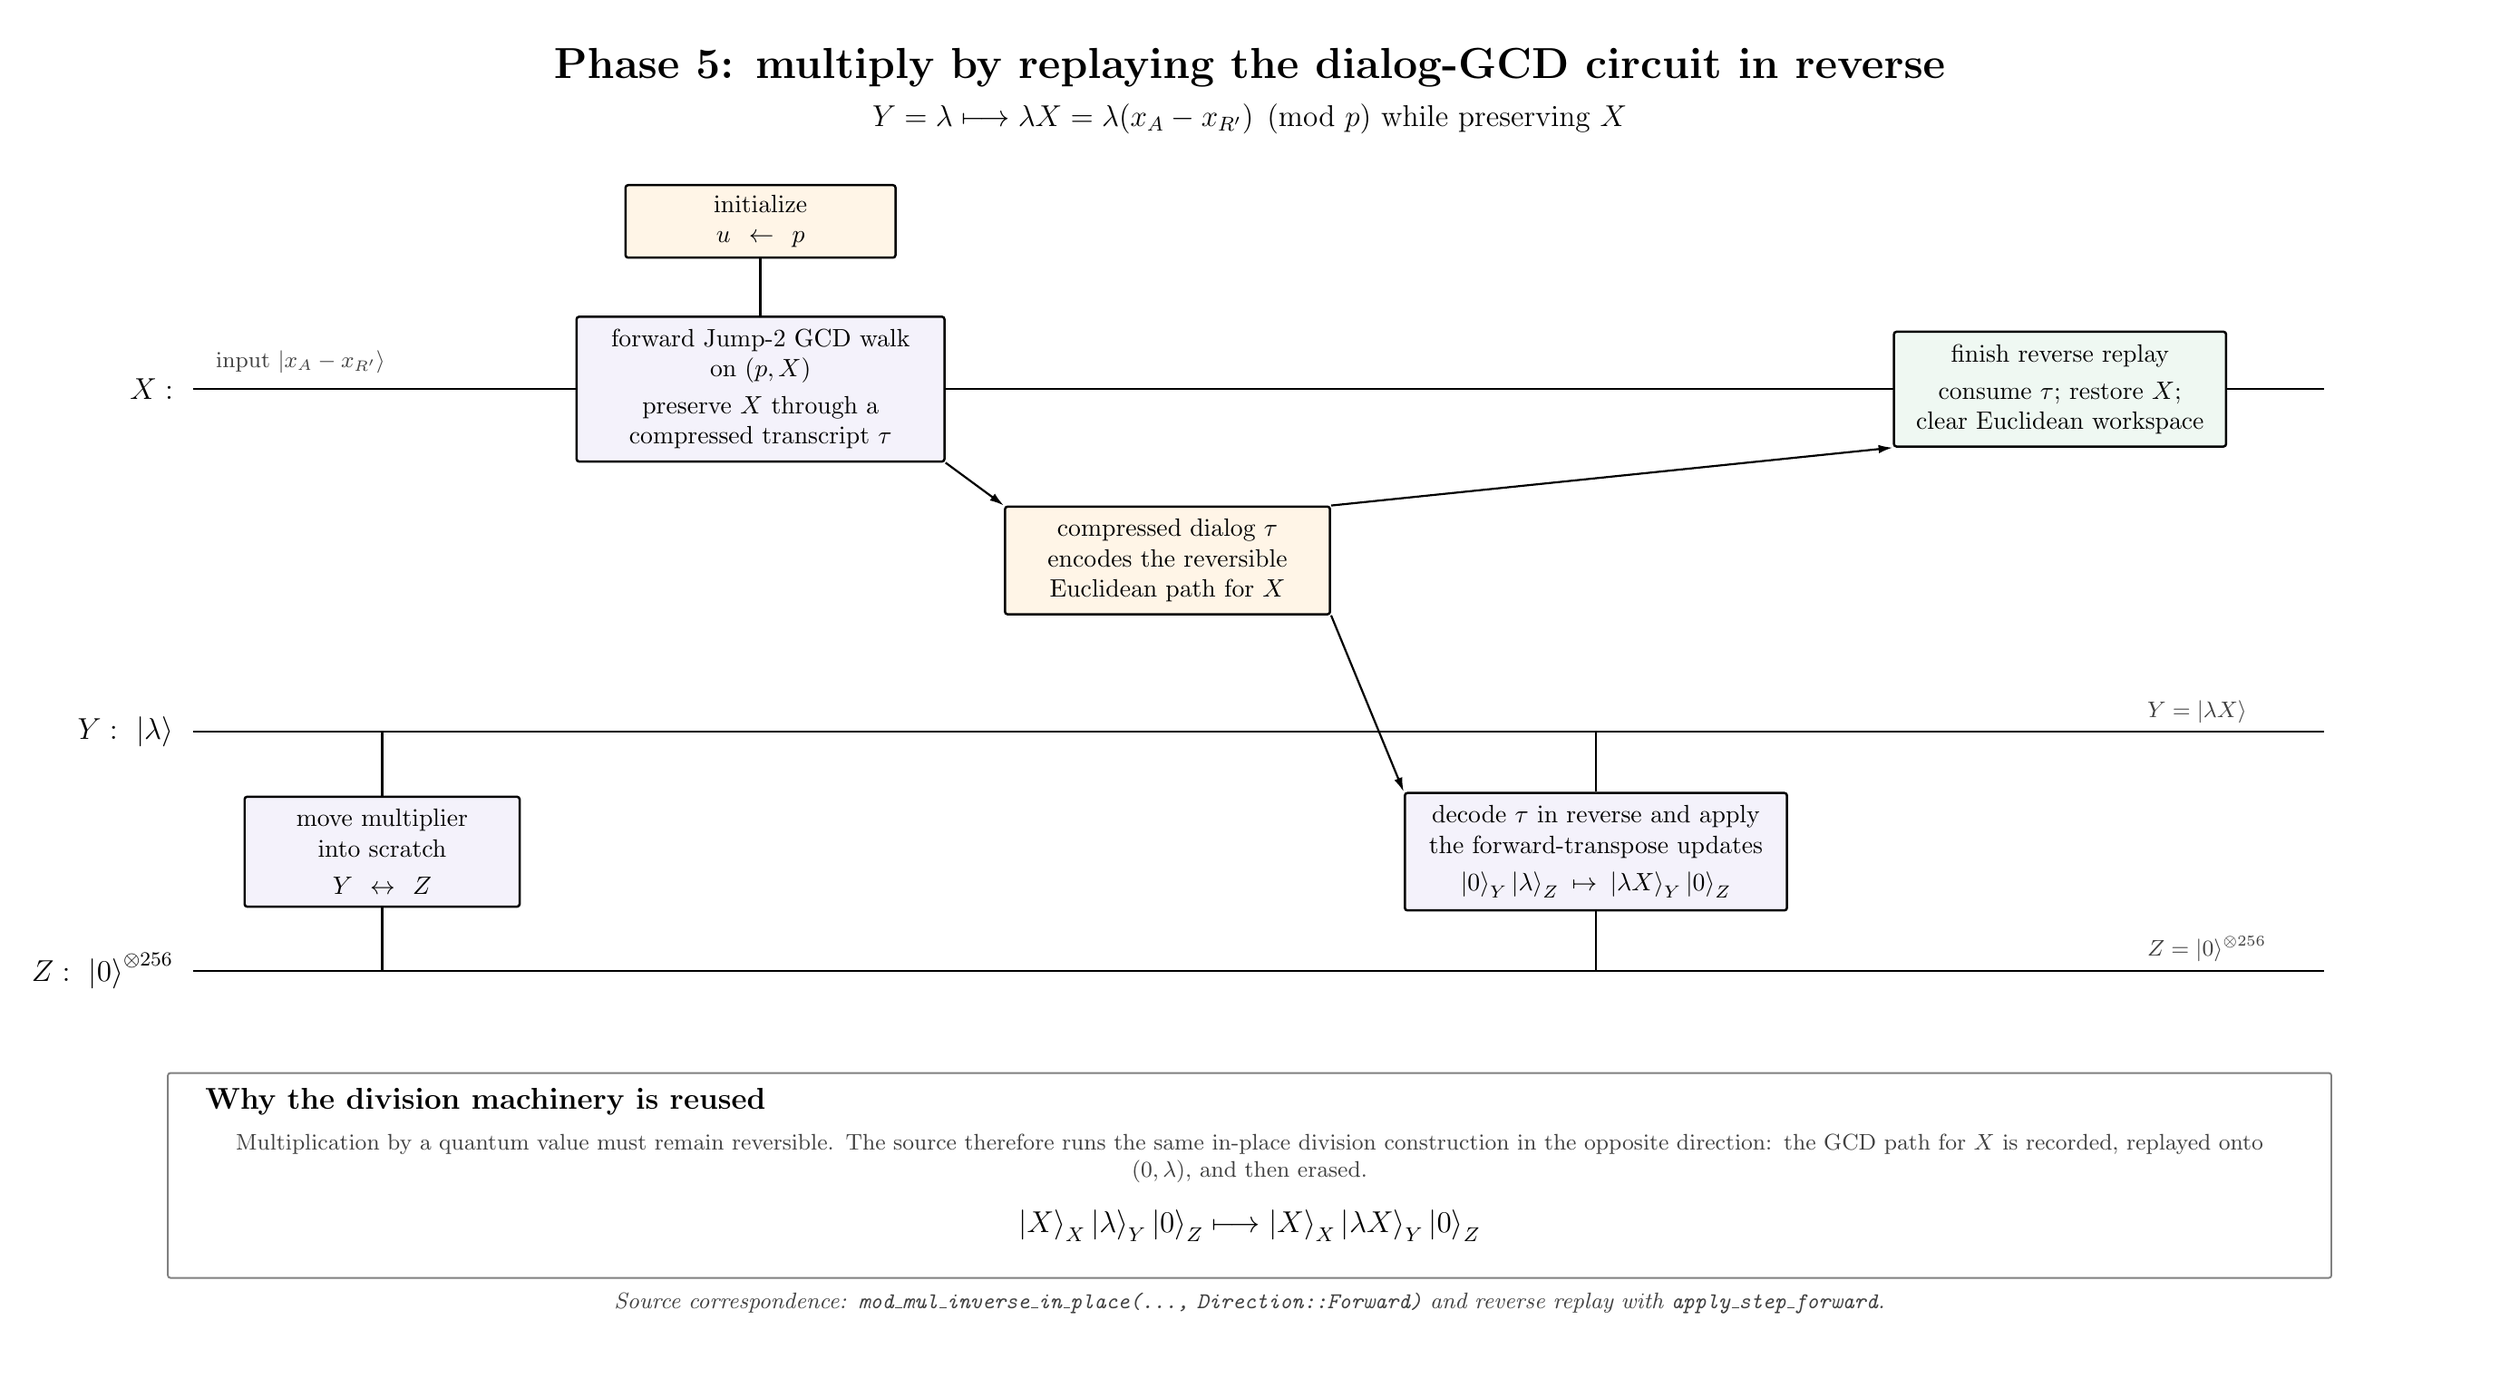
\begin{tikzpicture}[x=1cm,y=1cm]
  \path[use as bounding box] (0,0) rectangle (34.3,18.6);

  \node[font=\LARGE\bfseries] at (17.15,18.0)
    {Phase 5: multiply by replaying the dialog-GCD circuit in reverse};
  \node[font=\large] at (17.15,17.28)
    {$Y=\lambda\longmapsto\lambda X=\lambda(x_A-x_{R'})\pmod p$ while preserving $X$};

  \node[lab, anchor=east] at (2.2,13.5) {$X:$};
  \node[note, anchor=west] at (2.55,13.88)
    {input $\ket{x_A-x_{R'}}$};
  \node[lab, anchor=east] at (2.2,8.7) {$Y:\ \ket{\lambda}$};
  \node[lab, anchor=east] at (2.2,5.35) {$Z:\ \ket{0}^{\otimes256}$};
  \draw[wire] (2.35,13.5) -- (32.2,13.5);
  \draw[wire] (2.35,8.7) -- (32.2,8.7);
  \draw[wire] (2.35,5.35) -- (32.2,5.35);

  \node[detailviolet, text width=35mm] (SW2) at (5.0,7.02)
    {move multiplier\\into scratch\\[1mm]
     $Y\leftrightarrow Z$};
  \draw[wire] (5.0,8.7) -- (SW2.north);
  \draw[wire] (5.0,5.35) -- (SW2.south);

  \node[detailviolet, text width=48mm] (WALK2) at (10.3,13.5)
    {forward Jump-2 GCD walk\\on $(p,X)$\\[1mm]
     preserve $X$ through a\\compressed transcript $\tau$};
  \node[lookup, text width=35mm] (PREG2) at (10.3,15.85)
    {initialize\\$u\gets p$};
  \draw[wire] (PREG2.south) -- (WALK2.north);

  \node[detailorange, text width=42mm] (TAPE2) at (16.0,11.1)
    {compressed dialog $\tau$\\encodes the reversible\\Euclidean path for $X$};
  \draw[flow] (WALK2.south east) -- (TAPE2.north west);

  \node[detailviolet, text width=50mm] (REPLAY2) at (22.0,7.02)
    {decode $\tau$ in reverse and apply\\the forward-transpose updates\\[1mm]
     $\ket{0}_Y\ket{\lambda}_Z\mapsto
      \ket{\lambda X}_Y\ket{0}_Z$};
  \draw[flow] (TAPE2.south east) -- (REPLAY2.north west);
  \draw[wire] (22.0,8.7) -- (REPLAY2.north);
  \draw[wire] (22.0,5.35) -- (REPLAY2.south);

  \node[detailgreen, text width=43mm] (CLEAN2) at (28.5,13.5)
    {finish reverse replay\\[1mm]
     consume $\tau$; restore $X$;\\
     clear Euclidean workspace};
  \draw[flow] (TAPE2.north east) -- (CLEAN2.south west);
  \node[note, anchor=south west] at (29.6,8.7) {$Y=\ket{\lambda X}$};
  \node[note, anchor=south west] at (29.6,5.35) {$Z=\ket{0}^{\otimes256}$};

  \draw[black!50, line width=0.7pt, rounded corners=1pt]
    (2.0,1.05) rectangle (32.3,3.92);
  \node[font=\large\bfseries, anchor=west] at (2.4,3.52)
    {Why the division machinery is reused};
  \node[note, text width=29cm, align=center] at (17.15,2.72)
    {Multiplication by a quantum value must remain reversible.  The source therefore runs the same in-place division construction in the opposite direction: the GCD path for $X$ is recorded, replayed onto $(0,\lambda)$, and then erased.};
  \node[font=\large] at (17.15,1.78)
    {$\ket{X}_X\ket{\lambda}_Y\ket{0}_Z
      \longmapsto
      \ket{X}_X\ket{\lambda X}_Y\ket{0}_Z$};
  \node[note, text width=29cm, align=center, font=\small\itshape] at (17.15,0.70)
    {Source correspondence: \texttt{mod\_mul\_inverse\_in\_place(..., Direction::Forward)} and reverse replay with \texttt{apply\_step\_forward}.};
\end{tikzpicture}

\newpage

% ============================================================================
% Page 14: phase 6, recover affine output
% ============================================================================
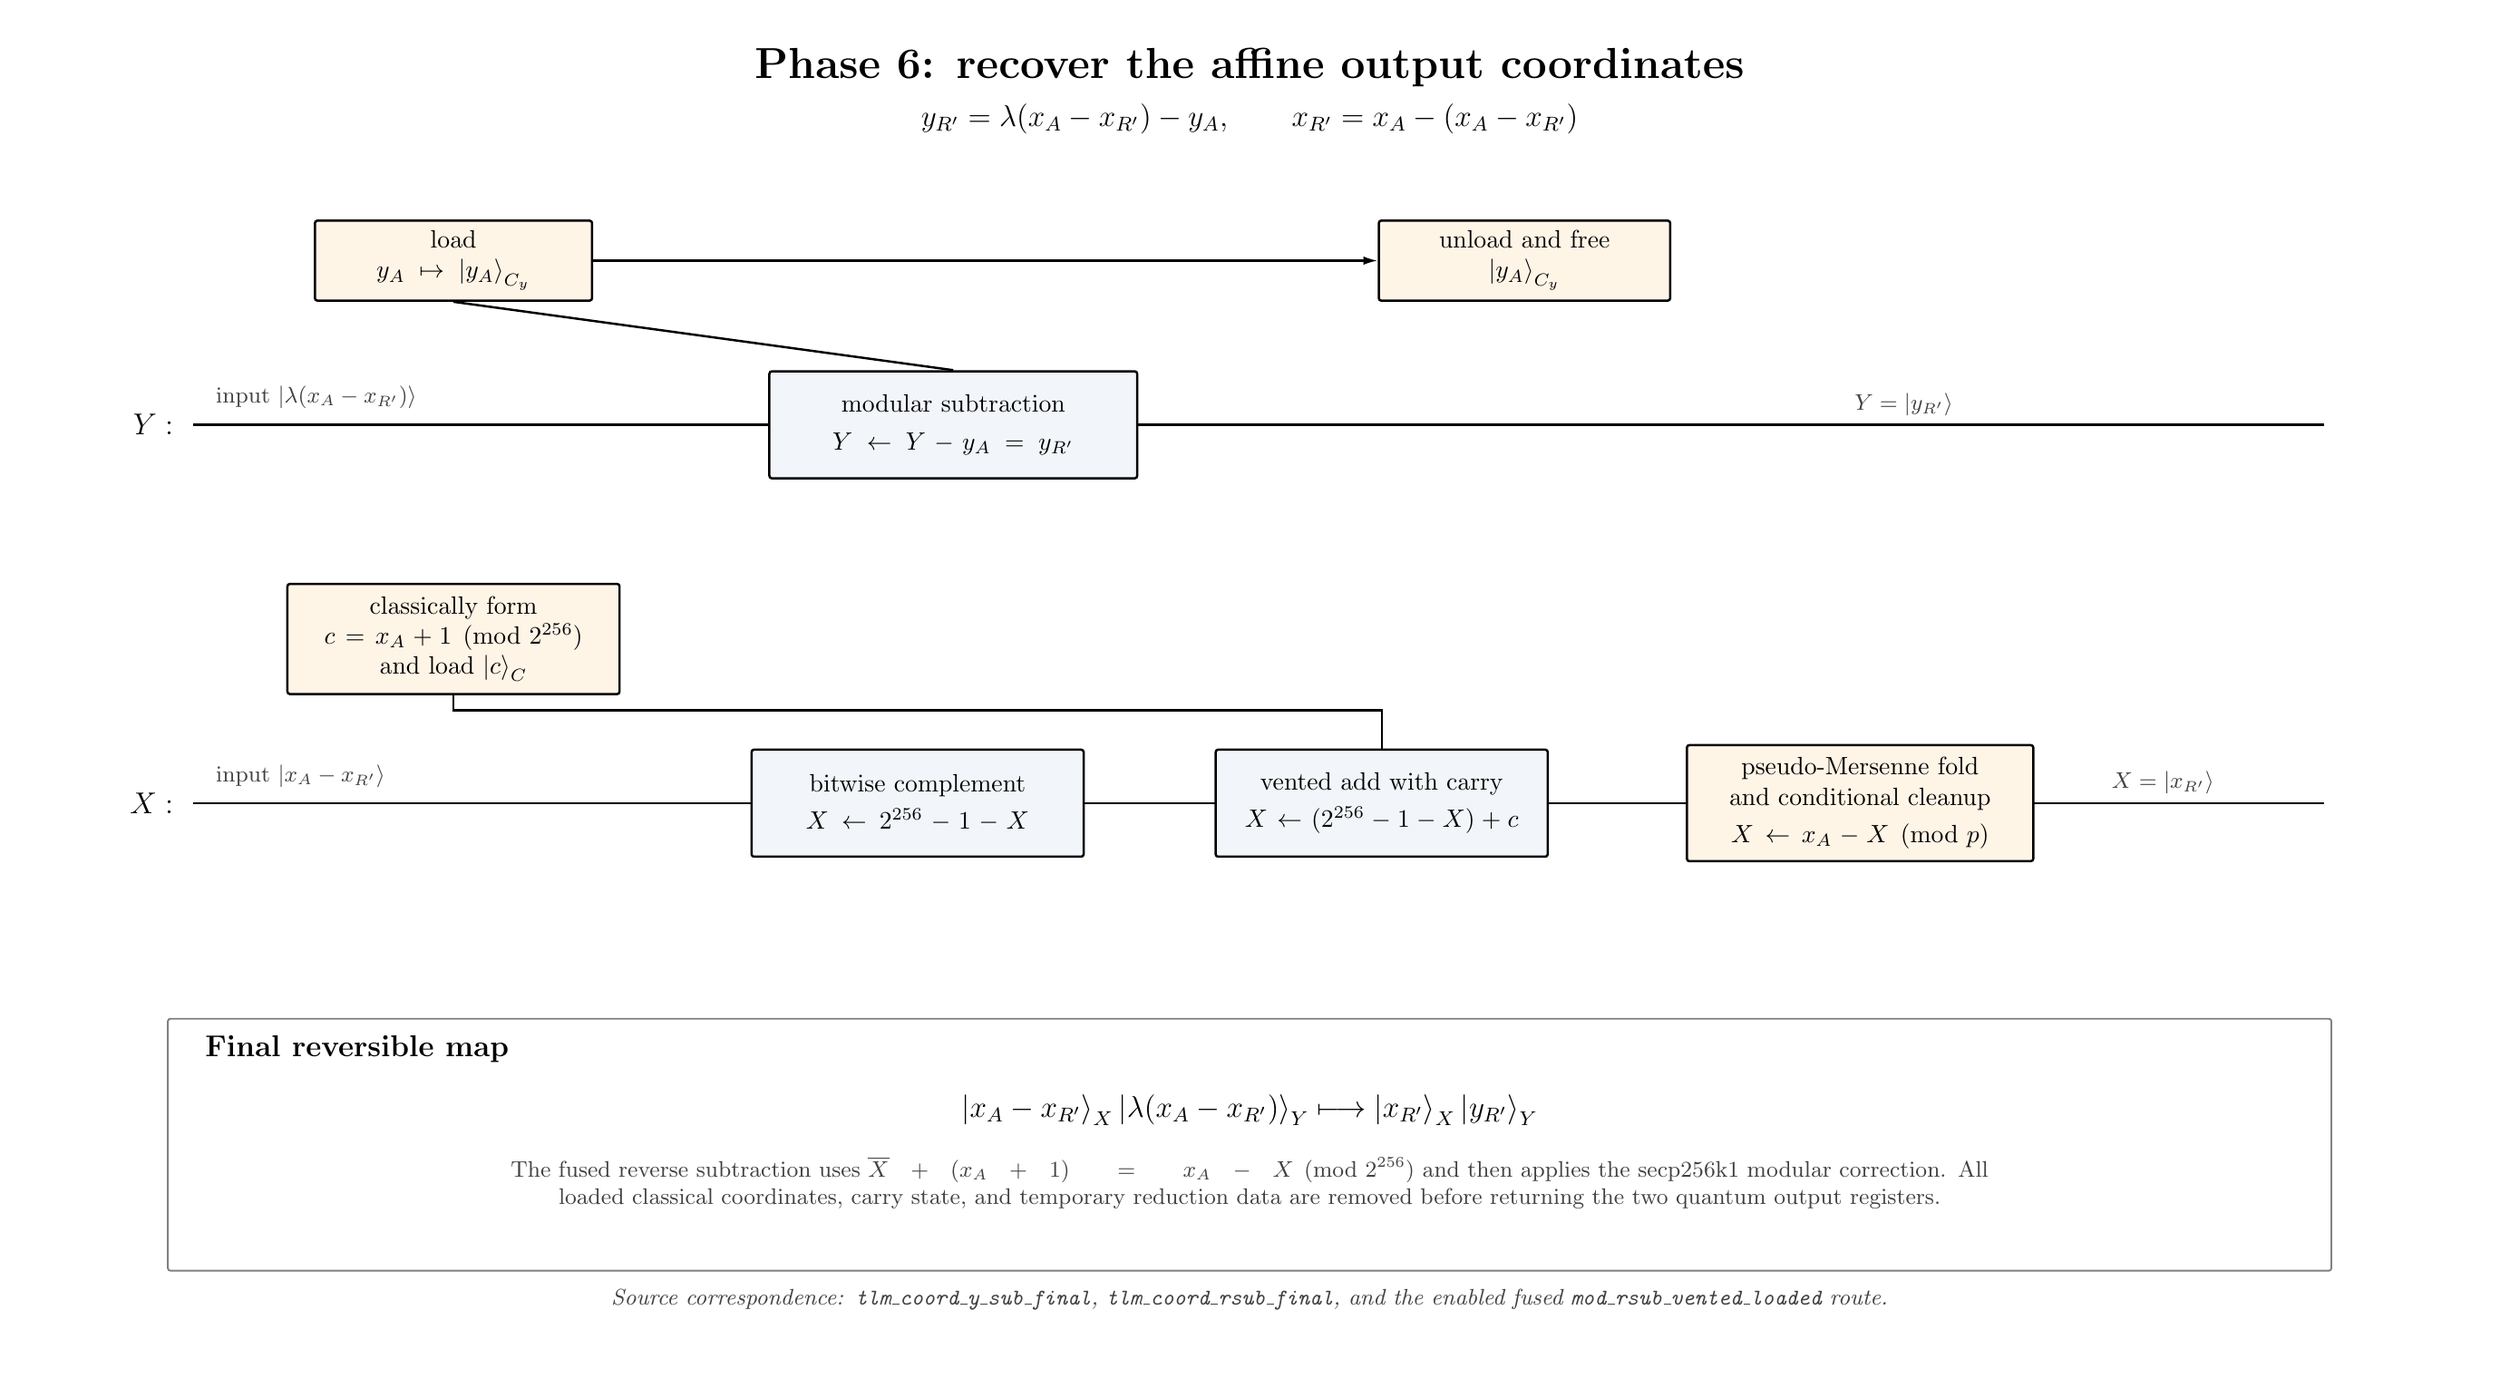
\begin{tikzpicture}[x=1cm,y=1cm]
  \path[use as bounding box] (0,0) rectangle (34.3,18.6);

  \node[font=\LARGE\bfseries] at (17.15,18.0)
    {Phase 6: recover the affine output coordinates};
  \node[font=\large] at (17.15,17.28)
    {$y_{R'}=\lambda(x_A-x_{R'})-y_A,\qquad x_{R'}=x_A-(x_A-x_{R'})$};

  % Y recovery lane.
  \node[lab, anchor=east] at (2.2,13.0) {$Y:$};
  \node[note, anchor=west] at (2.55,13.38)
    {input $\ket{\lambda(x_A-x_{R'})}$};
  \draw[wire] (2.35,13.0) -- (32.2,13.0);
  \node[lookup, text width=36mm] (LYF) at (6.0,15.3)
    {load\\$y_A\mapsto\ket{y_A}_{C_y}$};
  \node[detail, text width=48mm] (YSUB) at (13.0,13.0)
    {modular subtraction\\[1mm]
     $Y\gets Y-y_A=y_{R'}$};
  \draw[wire] (LYF.south) -- (YSUB.north);
  \node[lookup, text width=38mm] (UYF) at (21.0,15.3)
    {unload and free\\$\ket{y_A}_{C_y}$};
  \draw[flow] (LYF.east) -- (UYF.west);
  \node[note, anchor=south west] at (25.5,13.0) {$Y=\ket{y_{R'}}$};

  % X reverse-subtraction lane.
  \node[lab, anchor=east] at (2.2,7.7) {$X:$};
  \node[note, anchor=west] at (2.55,8.08)
    {input $\ket{x_A-x_{R'}}$};
  \draw[wire] (2.35,7.7) -- (32.2,7.7);
  \node[detailorange, text width=43mm] (PLUS1) at (6.0,10.0)
    {classically form\\$c=x_A+1\pmod{2^{256}}$\\and load $\ket c_C$};
  \node[detail, text width=43mm] (COMP) at (12.5,7.7)
    {bitwise complement\\[1mm]
     $X\gets 2^{256}-1-X$};
  \node[detail, text width=43mm] (RADD) at (19.0,7.7)
    {vented add with carry\\[1mm]
     $X\gets (2^{256}-1-X)+c$};
  \node[detailorange, text width=45mm] (FOLD) at (25.7,7.7)
    {pseudo-Mersenne fold\\and conditional cleanup\\[1mm]
     $X\gets x_A-X\pmod p$};
  \draw[wire] (PLUS1.south) -- (6.0,9.0) -- (19.0,9.0) -- (RADD.north);
  \node[note, anchor=south west] at (29.1,7.7) {$X=\ket{x_{R'}}$};

  \draw[black!50, line width=0.7pt, rounded corners=1pt]
    (2.0,1.15) rectangle (32.3,4.68);
  \node[font=\large\bfseries, anchor=west] at (2.4,4.25)
    {Final reversible map};
  \node[font=\large] at (17.15,3.40)
    {$\ket{x_A-x_{R'}}_X\ket{\lambda(x_A-x_{R'})}_Y
      \longmapsto
      \ket{x_{R'}}_X\ket{y_{R'}}_Y$};
  \node[note, text width=29cm, align=center] at (17.15,2.38)
    {The fused reverse subtraction uses $\overline X+(x_A+1)=x_A-X\pmod{2^{256}}$ and then applies the secp256k1 modular correction.  All loaded classical coordinates, carry state, and temporary reduction data are removed before returning the two quantum output registers.};
  \node[note, text width=29cm, align=center, font=\small\itshape] at (17.15,0.75)
    {Source correspondence: \texttt{tlm\_coord\_y\_sub\_final}, \texttt{tlm\_coord\_rsub\_final}, and the enabled fused \texttt{mod\_rsub\_vented\_loaded} route.};
\end{tikzpicture}

\end{document}
